
\documentclass[a4paper]{amsart}
\pdfoutput=1 % To make arXiv use pdflatex

% Att fixa
% -| "Separate" -> lägg till "for h, phi, ..." (Tog bort separate istället)
% - Indent in theorem
% -- p.10 c^phi -> d^phi
% - x and y på ellipse-axlarna
% - ta bort "to my knowledge"
% - Ta bort hypotes om evolute. (Eller iaf testa den numeriskt.)
% - Ta bort sin och cos serier ur theoremet och bara ha de i härledningen.
% - Decay rate of error ~e2? Den avtar ju med 0.01 för varje grad och det är ju ungerfär e2.
% - Kanske någon diskussion om att det borde gå att finna enklare uttryck samt att "h" verkar ha enklare form så att man borde kunna gå åt andra hållet. Detta visar dock på att det finns serie-expansioner.
% - Lägga till fler referenser till serie-expansioner för att visa att fler andra har försökt.

% Fixat (jämför med nedladdad .tex från arXiv för exakt diff)
% - Limits of "t" in d^phi.
% - Limit of innermost sum in d^{\sin}_{n,k,l} och d^{\sin}_{n,k,l} och d'_{n',k',l'}.
% - Upper limit of first sum of d^N_{n',k',l'}
% - min/max av fler än två.
% - adjusted some limits in coefficient tables.

% Att göra
% - Ändra d' till något bättre
% - Relation till kepler?
% - Bättre citering för Bell
% - Tydligare vad som är problemet med tidigare metoder?
% - Varför har expansionsnen för h enklast koefficienter?

% ArXiv
% - math.AG (Algebraic Geometry)
% - publicera med Python-variant initalt.
% - Lägg upp på arXiv först, Ladda sedan upp på github.

% Region of convergence.
% - If one converges, all converges. Prove convergence for \phi-\spi.
%	- Show that c^\phi < 1. Or decreasing?
% - All sums need to converge. On the other hand, convergence is dependent on limits of inner-more sums.
%	- Bound innermost sum and work form there...

% Files included in this document.
%  - bib-files:
%     - references.bib
%	  - (algorithm.bbl)
%  - figure-files:
%     - ellipse.pdf
%  - tables-files:
%     - c_latCosMul_table.tex
%     - c_latSinPow_table.tex
%     - c_altCosMul1_table.tex
%     - c_altCosMul2_table.tex
%     - c_altSinPow1_table.tex
%     - c_altSinPow2_table.tex
%     - c_sinPhiCosMul_table.tex
%     - c_sinPhiSinPow_table.tex
%     - c_cosPhiCosPow_table.tex
%     - c_cosPhiCosMul_table.tex

% For displaying address on the title page.
%\usepackage[foot]{amsaddr}
%\usepackage{amsaddr}
%\usepackage{amsmath} %aligned
%\usepackage{breqn}
\usepackage{amssymb}

% Displaying margins for debug.
%\usepackage{showframe}

\usepackage{tikz}

\usepackage[backend = biber,
    style = authoryear,
    giveninits = true,  % Shorten all first names.
    dashed = false,     % Prevent authors names from being replaced with dash.
    uniquename = false,  % This is just so that "Moritz, H." and "Moritz, Helmut" should not render extra initial to distinguish "different" authors.
    maxcitenames = 2  % To make three author list being cited as et al.
]{biblatex}
%\renewcommand*{\bibfont}{\normalfont\small}  % Make bibliografy font smaller. https://tex.stackexchange.com/questions/205432/with-biblatex-how-do-i-make-the-fontsize-of-the-bibliography-smaller
% This is to get the citation labels italic.
\DeclareCiteCommand{\cite}[\mkbibemph]
  {\usebibmacro{prenote}}%
  {\usebibmacro{citeindex}%
   \usebibmacro{cite}}
  {\multicitedelim}
  {\usebibmacro{postnote}}
\newcommand*{\mkbibemphparens}[1]{\mkbibparens{\mkbibemph{#1}}}
%
\addbibresource{references.bib}

% This is a filter to get a separate reference list for the appendix.
% See https://tex.stackexchange.com/questions/617195/separate-references-for-appendix-without-duplicates-with-main-body-automatical
\defbibfilter{appendixOnlyFilter}{
  segment=1 % Segment 1 will be chosen to be the one in appendix
  and not segment=0 % Default segment is 0
}
% Fontsize of bibliography.
\AtBeginBibliography{\small}  % Make bibliografy font smaller.
%\AtBeginBibliography{\footnotesize}  % Make bibliografy font smaller.

\usepackage{tabularx,ragged2e} % For automatically determining the column widths.
\usepackage{hyperref}  % URL in references and internal links.
\usepackage{graphicx}  % Floats and resizing table and symbols.
\usepackage[font=footnotesize]{caption}   %
\usepackage{mathtools} % For adjusted matrices.
\usepackage{longtable} % For tables spanning more than one page.

% This is to get "p" figures on a separat page.
\renewcommand\floatpagefraction{0} %default 0.5

\DeclareMathOperator{\atantwo}{atan2}

\title{Point-to-ellipse Fourier series}
\author{John-Olof Nilsson}%\\{\scriptsize A\lowercase{vioniq} S\lowercase{weden} AB, \lowercase{jnil02@kth.se}}}
%\author{John-Olof Nilsson}
%\address{The author is with Avioniq Sweden AB, e-mail: john\_nil@hotmail.com}
\address{John-Olof Nilsson is with Avioniq Sweden AB, e-mail: john\_nil@hotmail.com}
%\email{johnolof.nilsson@avioniq.se}
\date{}

%\usepackage[foot]{amsaddr} % To place address in footnote.

% To place address at specific point.
%\makeatletter
%\newcommand{\addresseshere}{%
%  \enddoc@text\let\enddoc@text\relax
%}
%\makeatother

\newtheorem{thm}{Theorem}

\begin{document}

\begin{abstract}
Fourier series with power series coefficients for the normal and distance to a point from an ellipse are derived. These expressions are the first of their kind and opens up a range of analysis and computational possibilities.
\end{abstract}

\maketitle

\vspace{-10mm}

\section{Introduction}

%\vspace{-2mm}
\begin{center}
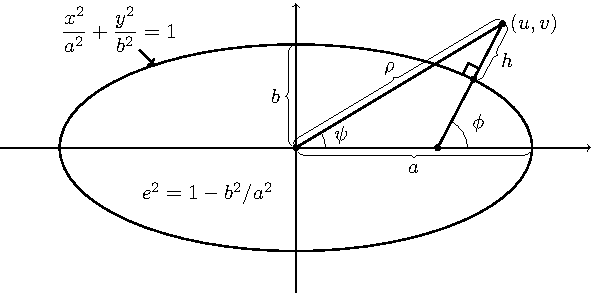
\includegraphics[]{ellipse.pdf}
\end{center}
%\vspace{-1mm}

\noindent
Determining the normal $\phi$ and the distance $h$ to a point $(u,v)$ from an ellipse with axes $a$ and $b$, as depicted above, is an extensively studied problem over the centuries:
%
Classical geometry techniques for the normal are known since the antiquity p.180~\cite{Heath1896};
%
Quartic equations
%, the so called latitude equation,
have been around since at least the early 1900-hundreds p.382~\cite{Gibson1911}, %p.49~\cite{Sommerville1924}, 
even if solid solution methods did not appear until recently~\cite{Vermeille2011};
%
100s of exact and approximate methods for computing $\phi$ and $h$ have been published since the 1960s~\cite{Nilsson2024}.
%
Despite this, only quartic equation, iterative, and closed-form approximation solutions are available, fundamentally limiting analysis and computations related to $\phi$ and $h$. 
%
%In contrast, here I provide
In contrast, provided here are
Fourier and power series in $\psi$ and $\sin(\psi)$ for $\phi$, $h$, and $\sin(\phi)$ and $\cos(\phi)$ (vector normal) whose coefficients are, in turn, power series
and polynomials
in $a/\rho$ and $e^2$ with rational coefficients.
%
The series are valuable in that:
\begin{itemize}
\item They are fundamental results for the ellipse conic and provide the first general series expansions for the point-to-ellipse relation.
\item Point-to-ellipse being a fundamental relation means that they enable series expansions of many related quantities.
%\item Many properties like parameter dependencies, 1\textsuperscript{st} and 2\textsuperscript{nd} order behaviors, limits, etc. become directly accessible.
\item They are differentiable, making updates for e.g. ellipse fitting, coordinate transformations, and differential equation solutions conceivable.
% Uncertainty handling.
\item Truncated series give simple algebraic approximations with potentially boundable errors and competitive performance.
\end{itemize}
Fourier series expansions have been attempted before by~\cite{Morrison1961} and \cite{Pick1967}, but these efforts have only resulted in a few initial and partial terms.
Series expansion inspiration is also drawn from~\cite{Nilsson2024minimax}.
%
The main limitation of this work is that no region of convergence is sought.
%The main limitation of this work is that series convergence is only ensured for sufficiently large $\tfrac{ae^2}{\rho\cos(\psi)}$.
%
The series are given in the next section. A brief discussion about them follows.
%
Finally, derivations, tabulated coefficients, and implementations are found in Appendices~\ref{app:A} and~\ref{sec::tabulated_coefficients} and \url{https://github.com/jnil02/point2ellipse_series}, respectively.

\section{The series}
The series are provided below in Fourier multiple-angle and $\sin$-power series forms. The former is fundamental and useful from a theoretical perspective whilst the latter brings more structure by reducing the innermost series to a polynomial. Further, the latter form is also more useful from a computational perspective since truncations directly give polynomials in the ratios $\varrho = a/\rho$, $\sin(\psi) = v / \rho$, and $\cos(\psi) = u /\rho$.

\vspace{3mm}
\begin{thm}
For the point-to-ellipse relation and sufficiently small $ae^2/u$
\vspace{1mm}
\begin{align*}
\phi-\psi &=\sum_{n=1}^\infty\left(\sum_{k=1}^\infty\left(\sum_{l=\max(n,k)}^\infty c^{\phi}_{n,k,l}e^{2l}\right)\varrho^k\right)\sin(2n\psi)\\
\frac{\phi-\psi}{\cos(\psi)\sin(\psi)}&=\sum_{n=0}^{\infty} \left(\sum_{k=1}^\infty\left(\sum_{l=\max(n+1,k)}^{n+k} d^{\phi}_{n,k,l}  e^{2l}\right)\varrho^k\right)\sin^{2n}(\psi)\\[2mm]
%
\frac{h + a - \rho}{a}
&=\sum_{n=0}^\infty\left(\sum_{k=0}^\infty\left(\sum_{l=\max(n,k+1)}^\infty c^h_{n,k,l}e^{2l}\right)\varrho^k\right)\cos(2n\psi)\\
&=\sum_{n=1}^\infty\left(\sum_{k=0}^\infty\left(\sum_{l=\max(n,k+1)}^{n+k} d^h_{n,k,l}e^{2l}\right)\varrho^k\right)\sin^{2n}(\psi)\\[2mm]
%
\frac{\sin(\phi)}{\sin(\psi)}-1&=\sum_{n=0}^\infty\left( \sum_{k=1}^\infty\left(\sum_{l=\max(n,k)}^\infty c^{\sin}_{n,k,l}e^{2l}\right)\varrho^k\right)\cos(2n\psi)\\
&=\sum_{n=0}^\infty\left( \sum_{k=1}^\infty\left(\sum_{l=\max(n,k)}^{n+k} d^{\sin}_{n,k,l}e^{2l}\right)\varrho^k\right)\sin^{2n}(\psi)\\[2mm]
%
\frac{\cos(\phi)}{\cos(\psi)}-1&=\sum_{n=0}^\infty\left( \sum_{k=1}^\infty\left(\sum_{l=\max(n,k)}^\infty c^{\cos}_{n,k,l}e^{2l}\right)\varrho^k\right)\cos(2n\psi)\\
&=\sum_{n=1}^\infty\left( \sum_{k=1}^\infty\left(\sum_{l=\max(n,k)}^{n+k-1} d^{\cos}_{n,k,l}e^{2l}\right)\varrho^k\right)\sin^{2n}(\psi)
\end{align*}
\vspace{1mm}
where the coefficients $c^{*}_{n,k,l}$ and $d^{*}_{n,k,l}$ are rational and, in order, given by the expressions \eqref{eq:c_phi}, \eqref{eq:d_phi}, \eqref{eq:c_h}, \eqref{eq:d_h}, \eqref{eq:c_sin}, \eqref{eq:d_sin}, \eqref{eq:c_cos}, and \eqref{eq:d_cos}, respectively.
\end{thm}
\begin{proof}
See Appendix~\ref{app:A}.
\end{proof}
\vspace{3mm}

\noindent
Note, in practice, the region of convergence appear to be of useful size, even including $u=0$ but not too small $\varrho$. Potentially it is outside the ellipse evolute.
%
Further note, the $\cos(\psi)\sin(\psi)$ in the $\sin$-power series of $\phi-\psi$ could easily be integrated into the series, but this gives a poor rate of convergence, see~\ref{app:phi}. %Even so, the series is ill conditioned close to $\phi=\pi/2$.
%
%Further, the $\cos(\phi)$ and $\sin(\phi)$ series are provided since $\cos(\phi)$ and $\sin(\phi)$ are often required rather than $\phi$. %, especially for computing $\phi$ close to $\pi/2$.
%
Finally, for computing both $\cos(\phi)$ and $\sin(\phi)$, it is preferable to compute them jointly with slightly different formulas, see~\ref{app:sincos}. For more computational details, see~\cite{Nilsson2024minimax}.

\section{Discussion}
To my knowledge, the series are the first general series expansions of $\phi$, $h$, $\sin(\phi)$, and $\cos(\phi)$ in terms of $\psi$ and $\rho$, or, alternatively, $u$ and $v$. Again, the series are:
\begin{itemize}
\item Essentially series solutions to the quartic latitude equation.%, which is interesting in the view of the recent~\cite{Wildberger2025}.
%\item Fourier series, or alternatively $\sin$-power series, with power series coefficients with, in turn, rational coefficients.
\item Series of fundamental relations, meaning that series for dependent quantities could be derived, enabling related analysis and computations. %The series for $h$ not involving $\phi$ and \emph{vice versa} are examples of this.
\item Trivially differentiable, both with respect to the point and the parameters, providing new paths for data fitting and transformation updates.
\item Easily approximated by truncation with granularly tuneable accuracy and potentially boundable errors for a given $\rho$. % meaning that a range of simple approximation methods could be implemented. %and implementable with interval arithmetic.
\end{itemize}
Hence, the series opens up a range of analysis and computational possibilities not obtainable from previous quartic equation, iterative, or closed-form approximate solutions.
%
Contributing to this are the $\sin$-power series variants, with its additional series structure. Depending on the use-case, $e^2$ may be a constant, e.g. geodesy, or a variable, e.g. ellipse fitting. %Hence, the actual (constant) coefficients are either the innermost sums or the rational coefficients.
For the latter case, this is obviously particularly valuable. For the former case, the $\sin$-power series structure is still valuable since $\sin^{2n}(\psi)$ is typically easier to evaluate for different $n$ than $\sin(2n\psi)$ and $\cos(2n\psi)$. %See~\cite{Nilsson2024minimax} for the subject of evaluating the truncated series.
%
%Note, $\cos$ power series %are straight-forward but
%brings no additional structure compared to the Fourier form (results not shown).
%
Unfortunately, the series come with some disadvantages:
\begin{itemize}
\item They appear not to converge for all points and ellipses and the region of convergence is so far not clear.
%\item The double/triple series nature means that even though the series appear to have geometric convergence with respect to $n$, they have subgeometric convergence with respect to arithmetic operations, i.e. other methods have better asymptotic convergence.
\item The series appear to have geometric convergence with respect to $n$ but, due to the inner series, subgeometric convergence with respect to arithmetic operations, i.e. other methods have better asymptotic convergence. % and many terms may be required for reasonable accuracy, i.e. computationally other methods may be more effective for a given accuracy.
\end{itemize}
However, convergence can probably be clarified and complementary series in $\varrho^{-1}$ could possibly be derived.
Further, series accelerations may possibly be applied.
Finally, for many practical applications, $e^2$ is small or $\rho$ is large giving fast initial convergence and potentially competitive performance for required accuracies.

%Any truncation will become more accurate the further away from the ellipse the point is.

%For some geometrical properties of the normal, see p.113-115~\cite{Akopyan2007}.

\section*{References}
\printbibliography[heading=none]
%\printbibliography[heading=none, segment=0] // With filtering.

\appendix
\newrefsegment %% <== increases the segment number (0 by default)


\section{Derivations}\label{app:A}
Let $(u,v)$ be a Cartesian coordinate of a point. Let $a$ and $b$ designate the major and minor axes of an ellipse aligned with the coordinate axes and centered at the origin. Let $h$ and $\phi$ designate the distance to the ellipse and the angle to the normal from the ellipse passing through $(u,v)$. Further, let $\rho=(u^2+v^2)^{1/2}$ and $\psi=\atantwo(v/u)$ be the polar coordinates of $(u,v)$. Then, from basic geometry,
\begin{align}
\label{eq:base1}
\rho\cos(\psi) &= (N + h)\cos(\phi)\\
\label{eq:base2}
\rho\sin(\psi) &= ((1-e^2)N + h)\sin(\phi)
\end{align}
where the eccentricity squared $e^2=1-b^2/a^2$ and the radius of curvature $N = a(1-e^2\sin(\phi))^{-1/2}$.
%
\eqref{eq:base1} and~\eqref{eq:base2} are the basis for the following series expansions derivations.
%
Further, in the derivation, the following formulas are used:
\newline
\emph{Lagrange reversion theorem}:
\begin{equation}
\begin{aligned}
\text{with}\quad y = x + d g(y),\quad\text{then for sufficiently small}\:d\\
f(y) = f(x) + \sum_{k=1}^{\infty}\frac{d^k}{k!}\left(\frac{\partial}{\partial x}\right)^{k-1}(f'(x)g^k(x))
\end{aligned}
\label{eq:lagrange}
\end{equation}
%
The \emph{general Leibniz rule}:
\begin{equation}
\frac{d^n}{dx^n}f(x)g(x) = \sum^n_{r=0}\binom{n}{r}\frac{d^{n-r}}{dx^{n-r}}f(x)\frac{d^r}{dx^r}g(x)\label{eq:leibniz}
\end{equation}
%
The \emph{Fa\'{a} di Bruno's formula}:
\begin{equation}
\frac{d^n}{dx^n}f(g(x))=\sum\frac{n!}{m_1!\dots m_n!} f^{(m_1+\dots+m_n)}(g(x))\prod_{i=1}^n\left(\frac{g^{(i)}(x)}{i!}\right)^{m_i}\label{eq:faa_di_bruno}
\end{equation}
%
%\subsection{Sin power series as a Fourier series}
Finally, for all but the $\phi$ expansion, the multi-angle Fourier expansions are obtained from the $\sin$-power expansions and the following relation. Let
\begin{equation*}
f(\phi) = \sum_{n=n_{\min}}^\infty \left(\sum_{k=k_{\min}}^\infty\left(\sum_{l=\max(n,k+k')}^{n+k+k''} e^{2l}d_{n,k,l}\right)\varrho^k\right)\sin^{2n}(\phi)
\end{equation*}
From the power reduction formulas
\begin{align*}
\sin^{2n}(\phi) &= \frac{1}{2^{2n}}\binom{2n}{n} + \frac{2}{2^{2n}}\sum_{i=0}^{n-1}(-1)^{n-i}\binom{2n}{i}\cos(2(n-i)\phi)
\end{align*}
Rearranging the sums gives
\begin{equation}
f(\phi)=\sum^\infty_{n=0}\left(\sum_{k=k_{\min}}^\infty\left(\sum_{l=\max(n,n_{\min},k+k')}^\infty e^{2l}c_{n,k,l}\right)\varrho^k\right)\cos(2n\phi)\label{eq:sinPowToCosMul}
\end{equation}
where %$\sum'$ means that the zeroth term is to be halved and
\begin{equation*}
c_{n,k,l}=\sum_{i=\max(n,n_{\min},l-k-k'')}^l d_{i,k,l}\frac{2}{2^{2i+\delta_n}}(-1)^{n}\binom{2i}{i-n}
\end{equation*}
where $\delta_*$ is the \emph{Kronecker delta}.
%
In the following subsections, expansions are derived for the desirable quantities and and some auxiliary quantities.

\subsection{Expansions for $\phi$}\label{app:phi}
Let $\varrho=a/\rho$. Dividing \eqref{eq:base2} by \eqref{eq:base1} and solving for $\tan(\phi)$
\begin{equation}\label{ref:base3}
\tan(\phi) = \tan(\psi) + \varrho\frac{e^2}{\cos(\psi)}\frac{\sin(\phi)}{(1 - e^2\sin^2(\phi))^{1/2}}
\end{equation}
Using the \emph{Lagrange reversion theorem}~\eqref{eq:lagrange} as in~\cite{Morrison1961} with
\begin{equation*}
y = \tan(\phi),\quad x=\tan(\psi)
\end{equation*}
\begin{equation*}
g(y)=\frac{y}{(1+(1-e^2)y^2)^{1/2}}=\frac{\sin(\phi)}{(1 - e^2\sin^2(\phi))^{1/2}}
\end{equation*}
\begin{equation*}
d = \varrho e^2(1+x^2)^{1/2}=\frac{\varrho e^2}{\cos(\psi)}
\end{equation*}
\begin{equation*}
\text{and}\quad f(y)=\tan^{-1}(y)
\end{equation*}
gives
\begin{equation*}
\tan^{-1}(y) = \tan^{-1}(x) + \sum_{k=1}^{\infty}\varrho^k\frac{e^{2k}(1+x^2)^{k/2}}{k!}\left(\frac{\partial}{\partial x}\right)^{k-1}\frac{x^k}{1+x^2}\frac{1}{(1+(1-e^2)x^2)^{k/2}}
\end{equation*}
To proceed beyond~\cite{Morrison1961}, an expression for the n\textsuperscript{th} derivative of the latter part is needed. Further, series expansions of $h$ and extra structure is enabled by derivation of alternative $\sin$-power series expansions. Finally, this expansion holds for \emph{sufficiently small} $d = \varrho e^2/\cos(\psi) = ae^2/u$.

The n\textsuperscript{th} derivative of $x^k$
\begin{equation*}
\frac{d^n}{dx^n}x^k =
\begin{cases}
\frac{k!}{(k-n)!}x^{k-n} & :n\leq k \\
0 & :n > k
\end{cases}
\end{equation*}
The n\textsuperscript{th} derivative of $\frac{1}{1+x^2}$
\begin{align*}
\frac{d^n}{dx^n}&\frac{1}{1+x^2} = \frac{d^n}{dx^n}\frac{1}{2i}\left(\frac{1}{x-i} - \frac{1}{x+i}\right)\\
&=(-1)^n\frac{n!}{2i}\left(\frac{1}{(x-i)^{n+1}} - \frac{1}{(x+i)^{n+1}}\right)\\
&=(-1)^n\frac{n!}{2i(x^2 + 1)^{n+1}}\left((x+i)^{n+1}-(x-i)^{n+1}\right)\\
&=(-1)^n\frac{n!}{2i(x^2 + 1)^{n+1}}\left(\sum^{n+1}_{k=0}\binom{n+1}{k}x^{n+1-k}i^k - \sum^{n+1}_{k=0}\binom{n+1}{k}x^{n+1-k}(-i)^k\right)\\
&=(-1)^n\frac{n!}{2i(x^2 + 1)^{n+1}}\sum^{n+1}_{k=0}\binom{n+1}{k}x^{n+1-k}i^k\left(1 - (-1)^k\right)\\
&=\frac{n!}{(x^2 + 1)^{n+1}}\sum^{n+1}_{k\in\mathbf{N}_o}\binom{n+1}{k}x^{n+1-k}(-1)^{n+(k-1)/2}\\
&=\sum^{n+1}_{k\in\mathbf{N}_o}(-1)^{n+(k-1)/2}n!\binom{n+1}{k}\frac{x^{n+1-k}}{(x^2 + 1)^{n+1}}\\
&=\sum^{\lfloor n/2\rfloor}_{k=0}(-1)^{n+k}n!\binom{n+1}{2k+1}\frac{x^{n-2k}}{(x^2 + 1)^{n+1}}
\end{align*}
where $\mathbf{N}_o$ designates the odd natural numbers.
%
Combining the expressions for $x^k$ and $\tfrac{1}{\smash{1+x^{{}_2}}}$ with the \emph{general Leibniz rule}~\eqref{eq:leibniz} gives the n\textsuperscript{th} derivative of $\tfrac{\smash{x^k}}{\smash{1+x^{{}_2}}}$
\begin{align*}
\frac{d^n}{dx^n}\frac{x^k}{1+x^2} &= \sum^n_{m=0}\binom{n}{m}\frac{k!}{(k-(n-m))!}x^{k-(n-m)}\\
&\quad\quad\sum^{\lfloor m/2\rfloor}_{p=0}(-1)^{m+p}m!\binom{m+1}{2p+1}\frac{x^{m-2p}}{(1 + x^2)^{m+1}}\\
& = \sum^n_{m=0}\sum^{\lfloor m/2\rfloor}_{p=0}\binom{m+1}{2p+1}\binom{k}{n-m}n!(-1)^{m+p}\frac{x^{m+1}}{(1 + x^2)^{m+1}}x^{k-n+m-2p-1}
\end{align*}
%
Required next is the n\textsuperscript{th} derivative of $\frac{1}{(1+(1-e^2)x^2)^{k/2}}$.
Trivially
\begin{equation*}
\frac{d^n}{dx^n}\frac{1}{(1+x)^{k/2}} = (-1)^n(k/2)^{\overline{n}}\frac{1}{(1+x)^{k/2+n}}
\end{equation*}
where $(\cdot)^{\overline{n}}$ indicates the rising factorial. Further
\begin{equation*}
\frac{d^n}{dx^n}(1-e^2)x^2 =
\begin{cases}
0 & \text{if}\quad n > 2 \\
\frac{2!}{(2-n)!}(1-e^2)x^{2-n} &  \text{otherwise}
\end{cases}
\end{equation*}
Plugging this into the \emph{Fa\'{a} di Bruno's formula}~\eqref{eq:faa_di_bruno} where the sum is over all partitions $m_1+2m_2+\dots+nm_n = n$, with $f(x)=\frac{1}{\smash{(1+x)^{{}_{k/2}}}}$ and $g(x)=(1-e^2)x^2$ and noting that the derivative of $g(x)=(1-e^2)x^2$ equals zero for $n>2$ which means that $m_n=0\forall n>2$, $m_1+2m_2=n$ and $m_2\in[0,\lfloor n/2\rfloor]$, giving
\begin{align*}
\frac{d^n}{dx^n}&\frac{1}{(1+(1-e^2)x^2)^{k/2}}\\
&=\sum\frac{n!}{m_1!m_2!} (-1)^{m_1+m_2}(k/2)^{\overline{m_1+m_2}}\frac{(2(1-e^2)x)^{m_1}(1-e^2)^{m_2}}{(1+(1-e^2)x^2)^{k/2+(m_1+m_2)}}\\
&=\sum_{m_2=0}^{\lfloor n/2\rfloor}\frac{n!(k/2)^{\overline{n-m_2}}}{(n-2m_2)!m_2!} (-1)^{n-m_2}\frac{(2(1-e^2)x)^{(n-2m_2)}(1-e^2)^{m_2}}{(1+(1-e^2)x^2)^{k/2+(n-m_2)}}\\
&=\sum_{m=0}^{\lfloor n/2\rfloor}(-1)^{n-m}\frac{n!(k/2)^{\overline{n-m}}2^{(n-2m)}}{(n-2m)!m!}\frac{(1-e^2)^{(n-m)}x^{(n-2m)}}{(1+(1-e^2)x^2)^{k/2+(n-m)}}
\end{align*}
%
Again, applying the \emph{general Leibniz rule} with the factors $\frac{\smash{x^k}}{\smash{1+x^{{}_2}}}$ and $\frac{1}{\smash{(1 + (1-e^{{}_2})x^{{}_2})^{{}_{k/2}}}}$ and expanding $(1-e^2)^{r-q}$ in a binomial sum gives the k\textsuperscript{th} term of the Lagrange reversion expansion
\begin{align}
&\varrho^k\frac{e^{2k}(1+x^2)^{k/2}}{k!}\left(\frac{\partial}{\partial x}\right)^{k-1}\frac{x^k}{1+x^2}\frac{1}{(1+(1-e^2)x^2)^{k/2}}\nonumber\\
&\quad\quad= \varrho^k\frac{e^{2k}(1+x^2)^{k/2}}{k!}\sum^{k-1}_{r=0}\binom{k-1}{r}\frac{d^{k-1-r}}{dx^{k-1-r}}\frac{x^k}{1+x^2}\frac{d^r}{dx^r}\frac{1}{(1 + (1-e^2)x^2)^{k/2}}\nonumber\\
&\quad\quad=\varrho^k\frac{e^{2k}(1+x^2)^{k/2}}{k!}\sum^{k-1}_{r=0}\binom{k-1}{r}\sum^{k-1-r}_{m=0}\sum^{\lfloor m/2\rfloor}_{p=0}\binom{m+1}{2p+1}\binom{k}{k-1-r-m}\nonumber\\
&\quad\quad\quad\quad\quad\quad(k-1-r)!(-1)^{m+p}\frac{x^{m+1}}{(1 + x^2)^{m+1}}x^{k-(k-1-r)+m-2p-1}\nonumber\\
&\quad\quad\quad\quad\quad\quad\quad\quad\quad\quad\sum_{q=0}^{\lfloor r/2\rfloor}(-1)^{r-q}\frac{r!(k/2)^{\overline{r-q}}2^{(r-2q)}}{(r-2q)!q!}\frac{(1-e^2)^{(r-q)}x^{(r-2q)}}{(1+(1-e^2)x^2)^{k/2+(r-q)}}\nonumber\\
&\quad\quad=\varrho^k\sum^{k-1}_{r=0}\sum^{k-1-r}_{m=0}\sum^{\lfloor m/2\rfloor}_{p=0}\sum_{q=0}^{\lfloor r/2\rfloor}\sum_{t=0}^{r-q}(-1)^{r-q+m+p+t}\frac{(k/2)^{\overline{r-q}}2^{(r-2q)}e^{2(t+k)}}{(r-2q)!q!(1+r+m)}\binom{r-q}{t}\raisetag{-8.75mm}\label{eq:lagrange_tot}\\
&\quad\quad\quad\binom{k-1}{r+m}\binom{m+1}{2p+1}x^{-2p-1}\!\left(\frac{x^2}{1 + x^2}\right)^{m+1-k/2}\!\left(\frac{x}{(1+(1-e^2)x^2)^{1/2}}\right)^{k+2(r-q)}\nonumber
\end{align}
Substitute $\tan(\phi)$ back for $x$, applying binomial expansion of $\frac{1}{(1-e^2\sin^2(\phi))}$, and collecting $\sin$ and $\cos$ factors gives the $x$ factors of~\eqref{eq:lagrange_tot}
\begin{align}
\nonumber
x^{-(2p+1)}&\left(\frac{x^2}{1 + x^2}\right)^{m+1-k/2}\left(\frac{x}{(1+(1-e^2)x^2)^{1/2}}\right)^{k+2(r-q)}\\
\nonumber
&=\tan^{-(2p+1)}(\phi)\sin^{2(m+1-k/2)}(\phi)\frac{\sin^{k+2(r-q)}(\phi)}{(1-e^2\sin^2(\phi))^{(k+2(r-q))/2}}\\
\label{eq:lat_split}
&=\sum_{s=0}^\infty\binom{\frac{k}{2}+r-q+s-1}{s}e^{2s}\cos^{2p+1}(\phi)\sin^{2(m+r-q+s-p)+1}(\phi)
\end{align}
From here the derivations of the Fourier multi-angle and the $\sin$-power series forms split. For the Fourier multi-angle, proceed from~\eqref{eq:lat_split} by applying the trigonometric power-reduction and product-to-sum formulas
\begin{align*}
x^{-(2p+1)}&\left(\frac{x^2}{1 + x^2}\right)^{m+1-k/2}\left(\frac{x}{(1+(1-e^2)x^2)^{1/2}}\right)^{k+2(r-q)}\\
&=\sum_{s=0}^\infty\binom{\frac{k}{2}+r-q+s-1}{s}e^{2s}
\frac{2}{2^{2p+1}}\sum_i^{p}\binom{2p+1}{i}\cos((2p+1-2i)\phi)\\
&\quad\quad\frac{2}{2^{2(m+r-q+s-p)+1}}\sum_j^{m+r-q+s-p}(-1)^{m+r-q+s-p-j}\\
&\quad\quad\binom{2(m+r-q+s-p)+1}{j}\sin((2(m+r-q+s-p)+1-2j)\phi)\\
%
&=\sum_{s=0}^\infty e^{2s}\sum_i^{p}\sum_j^w\binom{\frac{k}{2}+r-q+s-1}{s}\binom{2p+1}{i}\binom{2w+1}{j}
\frac{(-1)^{w-j}}{2^{2(w+p)+1}}\\
&\quad\quad\big(\sin(2(w-j+p-i+1)\phi) + \sin(2(w-j-(p-i))\phi)\big)
\end{align*}
where $w=m+r-q+s-p$. Inserting back into \eqref{eq:lagrange_tot} gives $\phi-\psi$ in terms of $\sin$-multiples
\begin{align*}
\phi-\psi = &\sum_{k=1}^\infty\sum_{s=0}^\infty\sum^{k-1}_{r=0}\sum^{k-1-r}_{m=0}\sum^{\lfloor m/2\rfloor}_{p=0}\sum_{q=0}^{\lfloor r/2\rfloor}\!\sum_{t=0}^{r-q}\sum_{i=0}^{p}\sum_{j=0}^{w}\varrho^k\frac{(-1)^{s-j+t}(k/2)^{\overline{r-q}}}{q!(r\!-\!2q)!(m\!+\!1\!+\!r)}\frac{e^{2(k+s+t)}}{2^{2(m+s)+r+1}}\\
&\binom{r-q}{t}\binom{k-1}{m+r}\binom{m+1}{2p+1}\binom{\frac{k}{2}+r-q+s-1}{s}\binom{2p+1}{i}\binom{2w+1}{j}\\
&\big(\sin(2(w-j+p-i+1)\phi) + \sin(2(w-j-(p-i))\phi)\big)
\end{align*}
To collect equal terms of $\sin(2n\psi)$, $e^{2l}$ and $\varrho^{k}$, note
\begin{itemize}
\item $w-j+p-i+1 \neq w-j-(p-i)$ so there is no $n=0$ term.
\item $l=s+k+t$ meaning that $s=l-k-t$.
\item $t$ is limited by $l$ since obviously $t+k\leq l$.
\item $w-j+p-i+1\in [1, k+s]$ meaning the first term can only contributes with a positive angle.
\item $w-j+p-i+1=n$ imply $j=w+p-i+1-n$ which, together with $j\in[0,w]$ and $i\in[0,p]$, imply $i\in[\max(0,p-n+1), \min(p, w+p-n+1)]$.
% w-j+p-i+1 = n
% j=w+p-i+1-n
% j in [0,w] => i >= p-n+1 och i <= w+p-n+1
\item $w-j-(p-i)\in [-\lceil (k-1)/2\rceil, k+s-1]$ so the second term can contribute with a positive and a negative term.
\item $w-j-(p-i)=n$ imply $j = w-p+i-n$ which, together with $j\in[0,w]$ and $i\in[0,p]$, imply $i\in[p-w+n, p]$.
% w-j-(p-i) = n
% j = w-p+i-n
% j in [0,w] => i >= p-w+n och i <= p+n (men i är redan mindre än p)
\item $w-j-(p-i)=-n$ imply $j = w-p+i+n$ which, together with $j\in[0,w]$ and $i\in[0,p]$, imply $i\in[p-w-n, p-n]$.
% w-j-(p-i) = -n
% j = w-p+i+n
% j in [0,w] => i >= p-w-n och i <= p-n
\item $l$ is obviously below limited by $k$, but also by $n$, since for a given $n$, $l\geq k+s\geq n$.
\end{itemize}
% Kan "p-w+n" bli 0?
% p-m-r+q-s+p+n = 2p+n-m+q-r
%
giving
\begin{align*}
\phi-\psi &= \sum_{n=1}^\infty\left(\sum_{k=1}^\infty\left(\sum_{l=\max(n,k)}^\infty c^\phi_{n,k,l}e^{2l}\right)\varrho^k\right)\sin(2n\phi)
\end{align*}
where the coefficients are given by
\begin{align}
c^\phi_{n,k,l}&=\sum^{k-1}_{r=0}\sum^{k-1-r}_{m=0}\sum^{\lfloor m/2\rfloor}_{p=0}\sum_{q=0}^{\lfloor r/2\rfloor}\sum_{t=0}^{\min(l-k,r-q)}\frac{(-1)^{l-k}(k/2)^{\overline{r-q}}}{q!(r-2q)!(m+1+r)2^{2(m+l-k-t)+r+1}}\nonumber\\
&\quad\quad\quad\quad\binom{r-q}{t}\binom{k-1}{m+r}\binom{m+1}{2p+1}\binom{\frac{k}{2}+r-q+l-k-t-1}{l-k-t}\nonumber\\
&\left(\sum_{i=\max(0,p-n+1)}^{\min(p, p-n+1+w)}(-1)^{w+p-i+1-n}\binom{2p+1}{i}\binom{2w+1}{w+p-i+1-n}\right.\nonumber\\
&\quad\quad\quad\quad\quad+\sum_{i=p-w+n}^{p}(-1)^{w-p+i-n}\binom{2p+1}{i}\binom{2w+1}{w-p+i-n}\nonumber\\
&\left.\quad\quad\quad\quad\quad\quad\quad\quad-\quad \sum_{i=p-w-n}^{p-n}(-1)^{w-p+i+n}\binom{2p+1}{i}\binom{2w+1}{w-p+i+n}\right)\label{eq:c_phi}
\end{align}
%This is clearly the Fourier series for the latitude with the innermost rational coefficients $c^\phi_{n,k,s}$ and the zero term equaling $\psi$.
%
In turn, the $\sin$-power series form is found by proceeding from~\eqref{eq:lat_split} as follows.
\begin{align*}
&x^{-(2p+1)}\left(\frac{x^2}{1 + x^2}\right)^{m+1-k/2}\left(\frac{x}{(1+(1-e^2)x^2)^{1/2}}\right)^{k+2(r-q)}\\
&=\cos(\phi)\sum_{s=0}^\infty\binom{\frac{k}{2}+r-q+s-1}{s}e^{2s}(1-\sin^{2}(\phi))^p\sin^{2(m+r-q+s-p)+1}(\phi)\\
&=\cos(\phi)\sum_{s=0}^\infty\binom{\frac{k}{2}+r-q+s-1}{s}e^{2s}\sum_{i=0}^{p}\binom{p}{i}(-1)^i\sin^{2i}(\phi)\sin^{2(m+r-q+s-p)+1}(\phi)\\
&=\cos(\phi)\sum_{s=0}^\infty e^{2s}\sum_{i=0}^{p}(-1)^i\binom{\frac{k}{2}+r-q+s-1}{s}\binom{p}{i}\sin^{2(m+r-q+s-p+i)+1}(\phi)\\
\end{align*}
Inserting back into~\eqref{eq:lagrange_tot} gives $\phi-\psi$ in terms of $\sin$-powers
\begin{align*}
\phi-\psi &= \cos(\phi)\sum_{k=1}^\infty\sum_{s=0}^\infty\sum^{k-1}_{r=0}\sum^{k-1-r}_{m=0}\sum^{\lfloor m/2\rfloor}_{p=0}\sum_{q=0}^{\lfloor r/2\rfloor}\sum_{t=0}^{r-q}\sum_{i=0}^{p}\varrho^k e^{2(k+s+t)}\\
&\quad\binom{r-q}{t}\binom{k-1}{m+r}\binom{m+1}{2p+1}\binom{\frac{k}{2}+r-q+s-1}{s}\binom{p}{i}\\
&\quad\frac{(-1)^{m+r-q+p+t+i}(k/2)^{\overline{r-q}}2^{r-2q}}{q!(r-2q)!(m+1+r)}\sin^{2(m+r-q+s-p+i)+1}(\phi)\\
\end{align*}
To collect equal terms of $\sin^{2n+1}(\psi)$, $e^{2l}$ and $\varrho^{k}$, note
\begin{itemize}
\item $l=s+k+t$ meaning that $s=l-k-t$.
\item $t$ is limited by $l$ and $k$ since obviously $t+k\leq l$.
\item $l$ is obviously below limited by $k$.
\item For a given $n$, from the $\sin$ factor $i = n - (m+r-q+s-p)$
\item For a given $n$ and $k$, $l$ is above limited since $n - (m+r-q+s-p) = i \geq 0$ implying $l \leq n+k$ and $t\geq l-n-k+m+r-p-q$.
\item For a given $k$, $l$ is below limited since $p \geq i = n - (m+r-q+s-p)$ implying $l \geq n+1$ and $t\leq l-n-k+m+r-q$, which in turn imply $t\geq0$.
\end{itemize}
giving
\begin{equation}\label{eq:latSinPow}
\frac{\phi-\psi}{\cos(\psi)\sin(\psi)} =\sum_{n=0}^{\infty} \left(\sum_{k=1}^\infty\left(\sum_{l=\max(n+1,k)}^{n+k} d^\phi_{n,k,l} e^{2l}\right)\varrho^k\right)\sin^{2n}(\psi)
\end{equation}
where
\begin{align}
d^\phi_{n,k,l}&=\sum^{k-1}_{r=0}\sum^{k-1-r}_{m=0}\sum^{\lfloor m/2\rfloor}_{p=0}\sum_{q=0}^{\lfloor r/2\rfloor}\sum_{t=l-n-k+m+r-p-q}^{\min(l-k,r-q,l-n-k+m+r-q)}\frac{(-1)^{n-l+k}(k/2)^{\overline{r-q}}2^{r-2q}}{q!(r-2q)!(m+1+r)}\nonumber\\
&\quad\binom{r\!-\!q}{t}\!\binom{k\!-\!1}{m\!+\!r}\!\binom{m\!+\!1}{2p\!+\!1}\!\binom{\frac{k}{2}\!+\!r\!-\!q\!+\!l\!-\!k\!-\!t\!-\!1}{l-k-t}\!\binom{p}{n\!-\!m\!-\!r\!+\!q\!-\!l\!+\!k\!+\!t\!+\!p}\raisetag{-7mm}\label{eq:d_phi}
\end{align}
Note, $\cos(\psi)$ in \eqref{eq:latSinPow} (and obiously $\sin(\psi)$) can easily be integrated into the series, by replacing the lower limit of $l$ with $k$ rather than $\max(n+1,k)$, removing the $t$ limit $t\leq l-n-k+m+r-q$ and replacing $p$ with $p+\frac{1}{2}$ in the last binomial of \eqref{eq:d_phi}. However, this gives a series with slow convergence limited by the expansion of $\cos(\psi)$. It is typically better to use $\cos(\psi)=(1-\smash{\sin}^2(\psi))^{1/2}$ and, therefore, such a series is not further explored.

\subsection{Expansions for $(\phi-\psi)^i$}
%As a stepping stone, series expansions for $(\phi-\psi)^n$ are needed.
For brevity, let
\begin{gather*}
a_{n,k}=\sum_{l=\max(n+1,k)}^{n+k} d^\phi_{n,k,l} e^{2l}\quad\text{and}\quad
a_n =\sum_{k=1}^\infty a_{n,k}\varrho^k%\\
%\text{i.e.}\quad\phi-\psi =\cos(\psi)\sin(\psi)\sum_{n=0}^{\infty} a_n\sin^{2n}(\psi)
\end{gather*}
Then, from~\eqref{eq:latSinPow}
\begin{align*}
(\phi-\psi)^i&=\cos^i(\psi)\sin^i(\psi)\left(\sum_{n=0}^\infty a_n\sin^{2n}(\psi)\right)^i\\
 &=\cos^i(\psi)\sin^i\sum_{n=0}^\infty b_{n,i}\sin^{2n}(\psi)
\end{align*}
where $b_{n,i}$ is a polynomial in $a_0,\dots,a_n$. The recurrence formula of powers of power series with non-zero constant term~\cite{Gould1974}, implicitly defines the \emph{ordinary potential polynomials}
\begin{align*}
b_{n,i} &=A_{n,i}(a_0,\dots,a_n) \\
&=
\begin{cases}
{a_0}^i& n=0\\
 \frac{1}{na_0}\sum_{k=1}^n(ki-n+k){a_k}b_{n-k,i}& n> 0
\end{cases}
\end{align*}
Further, since the series of $a_l$ has a zero constant term, its powers~\cite{Taghavian2023}%~p.366~\cite{Srivastava1992}
\begin{align*}
a_l^{i_l}=
\begin{cases}
1 & i_l = 0 \\
\sum_{k=i_l}^\infty \hat{B}_{k,i_l}(a_{l,1},\dots,a_{l,k-i_l+1})\varrho^k & i_l>0
\end{cases}
\end{align*}
where $\hat{B}_{k,i_l}(a_{l,1},\dots,a_{l,k-i_l+1})$ are the \emph{partial ordinary Bell polynomials} with a similar recurrence relation
\begin{equation*}
\hat{B}_{k,i}(x_1,\dots,x_{k-i+1})=
\begin{cases}
\delta_k & i = 0 \\
\sum_{j=1}^{k-i+1}x_j\hat{B}_{k-j,i-1}(x_1,\dots,x_{k-j-i}) & k \geq i, i \geq 1
\end{cases}
\end{equation*}
Finally, to collect equal terms of $e^{2l}$ and $\varrho^{k}$ in $b_{n,i}$, note
\begin{itemize}
\item For a given $i$, since $k$ starts at 1, the lowest power of $\varrho$ is $\varrho^i$.
\item For a given $k$, for each $a_{n,k}$ $l\geq k$ meaning that the power $e^{2l}$ is lower bounded by $k$.
\item For a given $n$, the lowest power of $e^2$ comes from multiplying the lowest powers in $a_l$. Writing $b_{n,i}$ as
\begin{equation*}
A_{n,i}(a_0,\dots,a_n)=b_{n,i}=\sum_{\substack{i_0+\dots+i_n=i \\ i_1+2i_2+\dots+ni_n=n}}\binom{i}{i_0,\dots,i_n}\prod_{l=0}^{i}a_l^{i_l}
\end{equation*}
and replacing each $a_l$ with the lowest power $e^{2(n+1)}$ gives
\begin{equation*}
\prod_{l=0}^{i}a_l^{i_l}\sim e^{2(i_0 + 2i_1+3i_2 + \dots+(n+1)i_n)}=e^{2(n+i)}
\end{equation*}
meaning that the power of $e^{2l}$ is lower bounded by $n+i$. %(Note, trivially the power is also lower bounded by $k$ but this limit does not affect affect the net result since $\max(n+i,k)=n+i$).
\item For a given $n$ and $k$, the highest power of $e^2$ is trivially bounded by $n+k$.
\end{itemize}
Consequently
\begin{equation*}
b_{n,i} = \sum_{k=i}^\infty\left(\sum_{l=\max(n+i,k)}^{n+k} d^\phi_{n,k,l,i}e^{2l}\right)\varrho^k
\end{equation*}
where
\begin{align*}
d^\phi_{n,k,l,i}&=[e^{2l}][\varrho^k]\left(A_ {n,i}(a_0,\dots,a_n)\left[a_n^{i_n}\rightarrow\sum_{k=i_n}^\infty \hat{B}_{k,i_n}(a_{n,1},\dots,a_{n,k-i_n+1})\varrho^k\right]\right)\\
&=[e^{2l}][\varrho^k]\left(\rule{0cm}{7mm}A_ {n,i}(a_0,\dots,a_n)\left[\rule{0cm}{7mm}a_n^{i_n}\rightarrow\right.\right.\\
&\!\!\!\!\left.\left.\sum_{k=i_n}^\infty \hat{B}_{k,i_n}\left(\sum_{l=\max(n+1,1)}^{n+1} d^\phi_{n,1,l} e^{2l},\dots,\sum_{l=\max(n+1,k-i_n+1)}^{n+k-i_n+1} d^\phi_{n,k-i_n+1,l} e^{2l}\right)\varrho^k\right]\right)
\end{align*}
% See https://groups.csail.mit.edu/mac/users/gjs/6.945/readings/Steele-MIT-April-2017.pdf for a note on substitute terminology.
where $[x^k]f(x)$ means the coefficient of $x^k$ in the series or polynomial $f(x)$ and $f(x)[x\rightarrow y]$ means the series or polynomial $f(x)$ with $x$ substituted with $y$. Note, the substitution of $a_n^{i_n}$ is done for all $n$ and $i_n$. Further, note, in determining $[x^k]f(x)$ in the coefficient expression above, the polynomials of the series have to be expanded with Cauchy products. %$c^\phi_{l,j,k,u}$ is a polynomial in $d_{n,k,l}$.
%
Combining it all gives
\begin{align}\label{eq:phiDiffPow}
(\phi-\psi)^i
 &=\cos^i(\psi)\sin^i\sum_{n=0}^\infty \left(\sum_{k=i}^\infty\left(\sum_{l=\max(n+i,k)}^{n+k} d^\phi_{n,k,l,i}e^{2l}\right)\varrho^k\right)\sin^{2n}(\psi)
\end{align}

\subsection{Expansions for $\sin(\phi)$ and $\cos(\phi)$}\label{app:sincos}
Expanding $\sin(\phi)$ in a Taylor series around $\psi$, using the $\sin$-power series expansion for $(\phi-\psi)^i$ from \eqref{eq:phiDiffPow} and expanding $\cos^{2x}(\psi)$ in $\sin^2(\psi)$ gives
\begin{align}
%\nonumber\frac{\sin(\phi)}{\sin(\psi)}&=\frac{\sin(\psi+\phi-\psi)}{\sin(\psi)}\\
\nonumber\frac{\sin(\phi)}{\sin(\psi)}&=\sum_{i=0}^\infty\frac{\partial}{\partial\varphi^i}\left.\frac{\sin(\varphi)}{i!}\right|_{\psi}\frac{1}{\sin(\psi)}(\phi-\psi)^i\\
\label{eq:sin_split}\raisetag{-7.5mm}&=\sum_{i\in\mathbf{N}_e}^\infty\frac{(-1)^{i/2}}{i!}(\phi-\psi)^i+\sum_{i\in\mathbf{N}_o}^\infty\frac{(-1)^{(i-1)/2}}{i!}\frac{\cos(\psi)}{\sin(\psi)}(\phi-\psi)^i\\
%&=\sum_{i}\in\mathbf{N}_e}^\infty\frac{(-1)^{i/2}}{i!}\cos^i(\psi)\sin^i\sum_{n=0}^\infty b_{n,i}\sin^{2n}(\psi)
%+\sum_{i\in\mathbf{N}_o}^\infty\frac{(-1)^{(i-1)/2}}{i!}\cos^{i+1}(\psi)\sin^{i-1}\sum_{n=0}^\infty b_{n,i}\sin^{2n}(\psi)\\
\nonumber&=1+\sum_{i=1}^\infty\frac{(-1)^{\lfloor i/2\rfloor}}{i!}\cos^{2\lceil i/2\rceil}(\psi)\sin^{2\lfloor i/2\rfloor}\sum_{n=0}^\infty b_{n,i}\sin^{2n}(\psi)\\
%&=1+\sum_{i=1}^\infty\frac{(-1)^{\lfloor i/2\rfloor}}{i!}(1-\sin^2(\psi))^{\lceil i/2\rceil}(\psi)\sin^{2\lfloor i/2\rfloor}\sum_{n=0}^\infty b_{n,i}\sin^{2n}(\psi)\\
%&=1+\sum_{i=1}^\infty\sum_{j=0}^{\lceil i/2\rceil}\binom{\lceil i/2\rceil}{j}\frac{(-1)^{\lfloor i/2\rfloor}}{i!}(-1)^j\sin^{2j}(\psi)\sin^{2\lfloor i/2\rfloor}\sum_{n=0}^\infty b_{n,i}\sin^{2n}(\psi)\\
\nonumber&=1+\sum_{i=1}^\infty\sum_{j=0}^{\lceil i/2\rceil}\binom{\lceil i/2\rceil}{j}\frac{(-1)^{\lfloor i/2\rfloor+j}}{i!}\sum_{n=0}^\infty b_{n,i}\sin^{2(n+\lfloor i/2\rfloor+j)}(\psi)\\
\nonumber&\!\!\!\!\!\!\!\!\!\!\!\!\!\!\!\!\!\!=1\!+\!\sum_{i=1}^\infty\!\sum_{j=0}^{\lceil i/2\rceil}\!\!\binom{\lceil i/2\rceil}{j}\frac{(-1)^{\lfloor i/2\rfloor\!+\!j}}{i!}\!\sum_{n=0}^\infty\! \left(\!\sum_{k=i}^\infty\!\left(\sum_{l=\max(n+i,k)}^{n+k}\!\!\!\!\!\!\!\!\! e^{2l}d^\phi_{n,k,l,i}\!\right)\!\varrho^k\!\right)\!\sin^{2(n\!+\!\lfloor i/2\rfloor\!+\!j)}(\psi)\\
\label{eq:sin}\raisetag{-9mm}&=1+\sum_{n=0}^\infty \left(\sum_{k=1}^\infty\left(\sum_{l=\max(n,k)}^{n+k} d^{\sin}_{n,k,l}e^{2l}\right)\varrho^k\right)\sin^{2n}(\psi)
\end{align}
where $\mathbf{N}_e$ and $\mathbf{N}_o$ designate the even and odd natural numbers and where
\begin{align}
\nonumber &d^{\sin}_{n',k',l'}\\
\nonumber &=\sum_{i=1}^\infty\!\sum_{j=0}^{\lceil i/2\rceil}\!\binom{\lceil i/2\rceil}{j}\frac{(-1)^{\lfloor i/2\rfloor\!+\!j}}{i!}\!\sum_{n=0}^\infty\! \left(\sum_{k=i}^\infty\!\left(\sum_{l=\max(n+i,k)}^{n+k}\!\!\!\!\! \delta_{l-l'}d^\phi_{n,k,l,i}\!\right)\!\delta_{k-k'}\!\right)\!\delta_{n\!+\!\lfloor i/2\rfloor\!+\!j-n'}\\
\raisetag{-9mm}&\quad\quad\quad=\sum_{i=1}^{\min(k',2n'+1)}\sum_{j=\max(0,\lceil i/2\rceil-l'+n')}^{\min(\lceil i/2\rceil,n'-\lfloor i/2\rfloor,n'+k'-l'-\lfloor i/2\rfloor)}\binom{\lceil i/2\rceil}{j}\frac{(-1)^{\lfloor i/2\rfloor+j}}{i!} d^\phi_{n'-\lfloor i/2\rfloor-j,k',l',i}\label{eq:d_sin}
\end{align}
where %$\delta_*$ is the \emph{Kronecker delta} and 
the summation limits are due to
\begin{itemize}
\item $\delta_{n+\lfloor i/2\rfloor+j-n'}$, $i\geq 1$, $j\geq 0$ and $n\geq 0$ imply
\begin{itemize}
\item $n'\geq 0$
\item $i\leq 2n'+1$
\item $j\leq n'-\lfloor i/2\rfloor$
\item $n = n'-\lfloor i/2\rfloor-j$
\end{itemize}
\item $\delta_{k-k'}$, $i\geq 1$ and $k\geq i$ imply
\begin{itemize}
\item $k'=k$
\item $k'\geq 1$
\item $i\leq k'$
\end{itemize}
\item $\delta_{l-l'}$ and $\max(n+i,k)\leq l\leq n+k$, imply
\begin{itemize}
\item $l'=l$
\item $i\leq l'-n= l'-n'+\lfloor i/2\rfloor+j$ meaning $\lceil i/2\rceil-l'+n'\leq j$
\item $l'\leq n + k' = n'+k'-\lfloor i/2\rfloor+j$ meaning $j\leq n'+k'-l'-\lfloor i/2\rfloor$
\item $\max(n',k')\leq l'\leq n'+k'$
\end{itemize}
\end{itemize}
Using~\eqref{eq:sinPowToCosMul}, the Fourier series follows as
\begin{equation}
\frac{\sin(\phi)}{\sin(\psi)}-1=\sum_{n=0}^\infty\left( \sum_{k=1}^\infty\left(\sum_{l=\max(n,k)}^\infty c^{\sin}_{n,k,l}e^{2l}\right)\varrho^k\right)\cos(2n\psi)
\end{equation}
where
\begin{equation}
c^{\sin}_{n,k,l}=\sum_{i=\max(n,l-k)}^l d^{\sin}_{i,k,l}\frac{2}{2^{2i+\delta_n}}(-1)^{n}\binom{2i}{i-n}\label{eq:c_sin}
\end{equation}

The derivation for $\cos(\phi)$ is identical with $\lfloor\cdot\rfloor$ changed to $\lceil\cdot\rceil$ and \emph{vice versa}, i.e.
\begin{align}
%\nonumber\frac{\cos(\phi)}{\cos(\psi)}&=\frac{\cos(\psi+\phi-\psi)}{\cos(\psi)}\\
\nonumber\frac{\cos(\phi)}{\cos(\psi)}&=\sum_{i=0}^\infty\frac{\partial}{\partial\varphi^i}\left.\frac{\cos(\varphi)}{i!}\right|_{\psi}\frac{1}{\cos(\psi)}(\phi-\psi)^i\\
\label{eq:cos_split}&=\sum_{i\in\mathbf{N}_e}^\infty\frac{(-1)^{i/2}}{i!}(\phi-\psi)^i-\frac{\sin^2(\psi)}{\cos^2(\psi)}\sum_{i\in\mathbf{N}_o}^\infty\frac{(-1)^{(i-1)/2}}{i!}\frac{\cos(\psi)}{\sin(\psi)}(\phi-\psi)^i\\
\label{eq:cos}&=1+\sum_{n=0}^\infty \left(\sum_{k=1}^\infty\left(\sum_{l=\max(n,k)}^{n+k-1} d^{\cos}_{n,k,l}e^{2l}\right)\varrho^k\right)\sin^{2n}(\psi)
\end{align}
where
\begin{equation}
d^{\cos}_{n',k',l'}=\sum_{i=1}^{\min(k',2n'+1)}\sum_{j=\max(0,\lfloor i/2\rfloor-l'+n')}^{\min(\lfloor i/2\rfloor,n'-\lceil i/2\rceil,n'+k'-l'-\lceil i/2\rceil)}\binom{\lfloor i/2\rfloor}{j}\frac{(-1)^{\lceil i/2\rceil+j}}{i!} d^\phi_{n'-\lceil i/2\rceil-j,k',l',i}\label{eq:d_cos}
\end{equation}
and
\begin{equation}
\frac{\cos(\phi)}{\cos(\psi)}-1=\sum_{n=0}^\infty\left( \sum_{k=1}^\infty\left(\sum_{l=\max(n,k)}^\infty c^{\cos}_{n,k,l}e^{2l}\right)\varrho^k\right)\cos(2n\psi)
\end{equation}
where
\begin{equation}
c^{\cos}_{n,k,l}=\sum_{i=\max(n,l-k+1)}^l d^{\cos}_{i,k,l}\frac{2}{2^{2i+\delta_n}}(-1)^{n}\binom{2i}{i-n}\label{eq:c_cos}
\end{equation}

Note, the reason \eqref{eq:sin_split} and \eqref{eq:cos_split} are spelt out is that if both $\sin(\phi)$ and $\cos(\phi)$ are to be computed, it may be preferable to use them. The reason is that~\eqref{eq:sin_split} and \eqref{eq:cos_split} are essentially univariate polynomials whereas~\eqref{eq:sin} and~\eqref{eq:cos} are bivariate polynomials. In addition, apart from the factor $-\tfrac{\smash{\sin^{{}_2}(\psi)}}{\smash{\cos^{{}_2}(\psi)}}$, they are identical. See~\cite{Nilsson2024minimax} for an example of such usage and some more comments about it.


\subsection{Expansions for $\cos(\phi-\psi)$}
Trivially
\begin{equation}
\cos(x) = 1 + \sum_{i=1}^\infty\frac{(-1)^i}{(2i)!}x^{2i}%\quad\forall |x|<\pi/2
\end{equation}
%Note that $|\phi-\psi|<\pi/2$.
Combining with \eqref{eq:phiDiffPow}
\begin{align}
\nonumber&\cos(\phi-\psi)\\
\nonumber&=1\!+\!\sum_{i=1}^\infty\frac{(-1)^i}{(2i)!}(1\!-\!\sin^2(\phi))^i\sin^{2i}(\phi)\!\sum_{n=0}^\infty \!\left(\sum_{k=2i}^\infty\!\left(\sum_{l=\max(n+2i,k)}^{n+k}\!\!\!\!\!\! d^\phi_{n,k,l,2i}e^{2l}\!\right)\!\varrho^k\!\right)\!\sin^{2n}(\psi)\\
%\nonumber&=1 + \sum_{i=1}^\infty\sum_{j=0}^i\frac{(-1)^{i}}{(2i)!}\binom{i}{j}(-1)^j\sin^{2j}(\phi)\sum_{n=0}^\infty\left(\sum_{k=2i}^\infty\left(\sum_{l=\max(n+2i,k)}^{n+k} d^\phi_{n,k,l,2i}e^{2l}\right)\varrho^k\right)\sin^{2n+2i}(\phi)\\
\nonumber&=1\!+\!\sum_{i=1}^\infty\sum_{j=0}^i\frac{(-1)^{i+j}}{(2i)!}\binom{i}{j}\sum_{n=0}^\infty\left(\sum_{k=2i}^\infty\left(\sum_{l=\max(n+2i,k)}^{n+k} e^{2l}d^\phi_{n,k,l,2i}\right)\!\varrho^k\!\right)\sin^{2n+2i+2j}(\phi)\\
\raisetag{-9mm}\label{eq:cosDiff}&\quad\quad\quad=1 + \sum_{n=1}^\infty\left(\sum_{k=2}^\infty\left(\sum_{l=\max(n,k)}^{n-1+k} d'_{n,k,l}e^{2l}\right)\varrho^k\right)\sin^{2n}(\phi)
\end{align}
where
\begin{align*}
d'_{n',k',l'}&=\sum_{i=1}^\infty\sum_{j=0}^i\!\frac{(-1)^{i+j}}{(2i)!}\binom{i}{j}\!\sum_{n=0}^\infty\!\left(\sum_{k=2i}^\infty\left(\sum_{l=\max(n+2i,k)}^{n+k}\!\!\!\!\! \delta_{l-l'}d^\phi_{n,k,l,2i}\!\right)\!\delta_{k-k'}\!\right)\!\delta_{n+i+j-n'}\\
%
&=\sum_{i=1}^{\min(n',\lfloor k'/2 \rfloor)}\sum_{j=\max(0,n'-l'+i)}^{\min(i,n'-i,n'+k'-l'-i)}\frac{(-1)^{i+j}}{(2i)!}\binom{i}{j}d^\phi_{n'-i-j,k',l',2i}
\end{align*}
The last equalities of the two proceeding equations are based on
\begin{itemize}
\item $\delta_{n+i+j-n'}$, $n\geq 0$ $i\geq 1$ and $0\leq j\leq i$ imply that
\begin{itemize}
\item $n'\geq 1$
\item $n = n'-i-j$
\item $0\leq j\leq n'-i$
\item $1\leq i\leq n'$
\end{itemize}
\item $\delta_{k-k'}$, $i\geq 1$, $k\geq 2i$ and $i\geq 1$ imply that
\begin{itemize}
\item $k'=k$
\item $k'\geq 2$
\item $i\leq \lfloor k'/2\rfloor$
\end{itemize}
\item $\delta_{l-l'}$, $\max(n+2i,k)\leq l\leq n+k$ and $j\leq i$ imply that
\begin{itemize}
\item $l'=l$
\item $n+2i\leq l$ meaning $j\geq n'-l'+ i$
\item $l\leq n+k$ meaning $j \leq n'+k'-l'-i$
\item $\max(n',k') \leq l' \leq n'-1+k'$
\end{itemize}
\end{itemize}

\subsection{Expansions for $(1-e^2\sin^2(\phi))^{1/2}$}
Applying binomial expansion twice
\begin{align*}
(1-e^2\sin^2(\phi))^{1/2}&=1 + \sum_{i=1}^\infty\binom{1/2}{i}(-1)^ie^{2i}\sin^{2i}(\phi)\\
%&=1 + \sum_{i=1}^\infty\binom{1/2}{i}(-1)^ie^{2i}\sin^{2i}(\psi)\left(\frac{\sin(\phi)}{\sin(\psi)}\right)^{2i}\\
&=1 + \sum_{i=1}^\infty\binom{1/2}{i}(-1)^ie^{2i}\sin^{2i}(\psi)\left(1+\left(\frac{\sin(\phi)}{\sin(\psi)}-1\right)\right)^{2i}\\
&=1 + \sum_{i=1}^\infty\binom{1/2}{i}(-1)^ie^{2i}\sin^{2i}(\psi)\sum_{j=0}^{2i}\binom{2i}{j}\left(\frac{\sin(\phi)}{\sin(\psi)}-1\right)^{j}
\end{align*}
Similar to the series expansion for $(\phi-\psi)^i$~\eqref{eq:phiDiffPow}, the last factor can be expanded with $\max(n+1,k)$ replaced with $\max(n,k)$, i.e.
\begin{align*}
\left(\frac{\sin(\phi)}{\sin(\psi)}-1\right)^j&=\left(\sum_{n=0}^\infty \left(\sum_{k=1}^\infty\left(\sum_{l=\max(n,k)}^{n+k} d^{\sin}_{n,k,l}e^{2l}\right)\varrho^k\right)\sin^{2n}(\psi)\right)^{j}\\
&=\sum_{n=0}^\infty \left(\sum_{k=j}^\infty\left(\sum_{l=\max(n,k)}^{n+k} d^{\sin}_{n,k,l,j}e^{2l}\right)\varrho^k\right)\sin^{2n}(\psi)
\end{align*}
where
\begin{align*}
d_{n,k,l,i}^{\sin}&=[e^{2l}][\varrho^k]\left(\rule{0cm}{7mm}A_{n,i}(a_0,\dots,a_n)\left[\rule{0cm}{7mm}a_n^{i_n}\rightarrow\right.\right.\\
&\!\!\!\!\left.\left.\sum_{k=i_n}^\infty \hat{B}_{k,i_n}\left(\sum_{l=\max(n,1)}^{n+1} d^{\sin}_{n,1,l} e^{2l},\dots,\sum_{l=\max(n,k-i_n+1)}^{n+k-i_n+1} d^{\sin}_{n,k-i_n+1,l} e^{2l}\right)\varrho^k\right]\right)
\end{align*}
This in turn gives
\begin{align*}
&(1-e^2\sin^2(\phi))^{1/2}\\
&=\sum_{i=1}^\infty\!\binom{1/2}{i}(-1)^ie^{2i}\sin^{2i}(\psi)\sum_{j=0}^{2i}\!\binom{2i}{j}\sum_{n=0}^\infty \left(\sum_{k=j}^\infty\left(\sum_{l=\max(n,k)}^{n+k}\!\!\!\!\! d^{\sin}_{n,k,l,j}e^{2l}\!\right)\!\varrho^k\right)\!\sin^{2n}(\psi)\\
&=\sum_{i=1}^\infty\binom{1/2}{i}(-1)^i\sum_{j=0}^{2i}\binom{2i}{j}\sum_{n=0}^\infty \left(\sum_{k=j}^\infty\left(\sum_{l=\max(n,k)}^{n+k} d^{\sin}_{n,k,l,j}e^{2(l+i)}\right)\varrho^k\right)\sin^{2(n+i)}(\psi)
\end{align*}
which may be written as a plain triple sum
\begin{equation}
(1-e^2\sin^2(\phi))^{1/2}=\sum_{n=1}^\infty \left(\sum_{k=0}^\infty\left(\sum_{l=\max(n,k+1)}^{n+k} d^{N}_{n,k,l}e^{2l}\right)\varrho^k\right)\sin^{2n}(\psi)\label{eq:N}
\end{equation}
where
\begin{align*}
d^N_{n',k',l'}&=\!\sum_{i=1}^\infty\!\binom{1/2}{i}(-1)^i\sum_{j=0}^{2i}\!\binom{2i}{j}\!\sum_{n=0}^\infty \!\left(\sum_{k=j}^\infty\left(\sum_{l=\max(n,k)}^{n+k}\!\!\!\!\! \delta_{l+i-l'}d^{\sin}_{n,k,l,j}\!\right)\!\delta_{k-k'}\!\right)\!\delta_{n+i-n'}\\
&=\sum_{i=1}^{n'}\binom{1/2}{i}(-1)^i\sum_{j=0}^{\min(2i,k')}\binom{2i}{j}d^{\sin}_{n'-i,k',l'-i,j}
\end{align*}
The last equalities of the two proceeding equations are based on
\begin{itemize}
\item $\delta_{n+i-n'}$, $n\geq 0$ and $i\geq1$  imply
\begin{itemize}
\item $n'\geq 1$
\item $1\leq i\leq n'$
\item $n=n'-i$
\end{itemize}
\item $\delta_{k-k'}$ and $k\geq j$ imply
\begin{itemize}
\item $k'=k$
\item $k'\geq 0$
\item $j\leq k'$
\end{itemize}
\item $\delta_{l+i-l'}$, $\max(n,k)\leq l\leq n+k$ and $j\leq 2i$ imply
\begin{itemize}
\item $l=l'-i$
\item $i= l'-l\leq l'$ but $l'>n'$ so this adds no constraint.
\item $\max(n'-i,k')\leq l'-i$, i.e. $\max(n',k'+1)\leq l'$
\item $l'-i\leq n'-i+k'$, i.e. $l'\leq n'+k'$
\end{itemize}
\end{itemize}


\subsection{Expansions for $h$}\label{app:h}
Multiplying \eqref{eq:base1} with $\cos(\phi)$ and \eqref{eq:base2} with $\sin(\phi)$, adding, simplifying and solving for $h$ gives 
\begin{equation*}
h=\rho\cos(\phi-\psi)-a(1-e^2\sin^2(\phi))^{1/2}
\end{equation*}
Combining with \eqref{eq:cosDiff} and \eqref{eq:N} directly gives
\begin{equation}
\frac{h + a - \varrho}{a} = \sum_{n=1}^\infty\left(\sum_{k=0}^\infty\left(\sum_{l=\max(n,k+1)}^{n+k} d^h_{n,k,l}e^{2l}\right)\varrho^k\right)\sin^{2n}(\phi)
\end{equation}
where
\begin{equation}
d^h_{n,k,l}=
\begin{cases}
-d^N_{n,k,l} & k=0 \\
d'_{n,k+1,l}-d^N_{n,k,l} & \text{otherwise}
\end{cases}\label{eq:d_h}
\end{equation}
Using~\eqref{eq:sinPowToCosMul}, the Fourier series follows as
\begin{equation}
\frac{h + a - \varrho}{a}=\sum_{n=0}^\infty\left( \sum_{k=0}^\infty\left(\sum_{l=\max(n,k+1)}^\infty c^h_{n,k,l}e^{2l}\right)\varrho^k\right)\cos(2n\psi)
\end{equation}
where
\begin{equation}
c^h_{n,k,l}=\sum_{i=\max(n,l-k)}^l d^h_{i,k,l}\frac{2}{2^{2i+\delta_n}}(-1)^{n}\binom{2i}{i-n}\label{eq:c_h}
\end{equation}

%\section*{Appendix references}\label{app:ref}
%\printbibliography[heading=none, filter=appendixOnlyFilter]

\section{Tabulated coefficients}\label{sec::tabulated_coefficients}
The rational series expansion coefficients, i.e. \eqref{eq:c_phi}, \eqref{eq:d_phi}, \eqref{eq:c_h}, \eqref{eq:d_h}, \eqref{eq:c_sin}, \eqref{eq:d_sin}, \eqref{eq:c_cos}, and \eqref{eq:d_cos}, are tabulated in Table~\ref{tab:c_phi}-\ref{tab:d_cos}. %Values outside the sum limits are indicated with a $\times$.

\begin{table}
\tiny
\begin{tabular}{ @{\hspace{0mm}} c@{\hspace{1mm}} c@{\hspace{1mm}} | @{\hspace{0mm}} l@{}  l@{}  l@{}  l@{}  l@{}  l@{}  l@{}  l@{} }
$n$ & $k\setminus l$ & $\phantom{{-}}e^{2\cdot1}$ & $\phantom{{-}}e^{2\cdot2}$ & $\phantom{{-}}e^{2\cdot3}$ & $\phantom{{-}}e^{2\cdot4}$ & $\phantom{{-}}e^{2\cdot5}$ & $\phantom{{-}}e^{2\cdot6}$ & $\phantom{{-}}e^{2\cdot7}$ & $\phantom{{-}}e^{2\cdot8}$ \\ \hline
 $\sin^{2\cdot1}(\psi)$ & $\varrho^{1}$  & $\phantom{-}1/2$  & $\phantom{-}1/8$  & $\phantom{-}15/256$  & $\phantom{-}35/1024$  & $\phantom{-}735/32768$  & $\phantom{-}2079/131072$  & $\phantom{-}99099/8388608$  & $\phantom{-}306735/33554432$  \\[-0.2mm]
 & $\varrho^{2}$  & $\phantom{-}\times$  & $\phantom{-}0$  & $\phantom{-}1/32$  & $\phantom{-}1/32$  & $\phantom{-}7/256$  & $\phantom{-}3/128$  & $\phantom{-}165/8192$  & $\phantom{-}143/8192$  \\[-0.2mm]
 & $\varrho^{3}$  & $\phantom{-}\times$  & $\phantom{-}\times$  & $-3/64$  & $-9/256$  & $-105/4096$  & $-315/16384$  & $-31185/2097152$  & $-99099/8388608$  \\[-0.2mm]
 & $\varrho^{4}$  & $\phantom{-}\times$  & $\phantom{-}\times$  & $\phantom{-}\times$  & $\phantom{-}0$  & $\phantom{-}0$  & $\phantom{-}0$  & $\phantom{-}0$  & $\phantom{-}0$  \\[-0.2mm]
 & $\varrho^{5}$  & $\phantom{-}\times$  & $\phantom{-}\times$  & $\phantom{-}\times$  & $\phantom{-}\times$  & $-5/2048$  & $-25/8192$  & $-1575/524288$  & $-5775/2097152$  \\[-0.2mm]
 & $\varrho^{6}$  & $\phantom{-}\times$  & $\phantom{-}\times$  & $\phantom{-}\times$  & $\phantom{-}\times$  & $\phantom{-}\times$  & $\phantom{-}0$  & $\phantom{-}0$  & $\phantom{-}0$  \\[-0.2mm]
 & $\varrho^{7}$  & $\phantom{-}\times$  & $\phantom{-}\times$  & $\phantom{-}\times$  & $\phantom{-}\times$  & $\phantom{-}\times$  & $\phantom{-}\times$  & $-35/131072$  & $-245/524288$  \\[-0.2mm]
 & $\varrho^{8}$  & $\phantom{-}\times$  & $\phantom{-}\times$  & $\phantom{-}\times$  & $\phantom{-}\times$  & $\phantom{-}\times$  & $\phantom{-}\times$  & $\phantom{-}\times$  & $\phantom{-}0$  \\[0.4mm]
\hline
 $\sin^{2\cdot2}(\psi)$ & $\varrho^{1}$  & $\phantom{-}\times$  & $-1/16$  & $-3/64$  & $-35/1024$  & $-105/4096$  & $-10395/524288$  & $-33033/2097152$  & $-429429/33554432$  \\[-0.2mm]
 & $\varrho^{2}$  & $\phantom{-}\times$  & $\phantom{-}1/4$  & $\phantom{-}1/8$  & $\phantom{-}1/16$  & $\phantom{-}1/32$  & $\phantom{-}15/1024$  & $\phantom{-}11/2048$  & $\phantom{-}0$  \\[-0.2mm]
 & $\varrho^{3}$  & $\phantom{-}\times$  & $\phantom{-}\times$  & $\phantom{-}0$  & $\phantom{-}15/256$  & $\phantom{-}75/1024$  & $\phantom{-}4725/65536$  & $\phantom{-}17325/262144$  & $\phantom{-}495495/8388608$  \\[-0.2mm]
 & $\varrho^{4}$  & $\phantom{-}\times$  & $\phantom{-}\times$  & $\phantom{-}\times$  & $-1/16$  & $-1/16$  & $-51/1024$  & $-19/512$  & $-55/2048$  \\[-0.2mm]
 & $\varrho^{5}$  & $\phantom{-}\times$  & $\phantom{-}\times$  & $\phantom{-}\times$  & $\phantom{-}\times$  & $\phantom{-}0$  & $-175/32768$  & $-1225/131072$  & $-24255/2097152$  \\[-0.2mm]
 & $\varrho^{6}$  & $\phantom{-}\times$  & $\phantom{-}\times$  & $\phantom{-}\times$  & $\phantom{-}\times$  & $\phantom{-}\times$  & $\phantom{-}0$  & $\phantom{-}0$  & $\phantom{-}0$  \\[-0.2mm]
 & $\varrho^{7}$  & $\phantom{-}\times$  & $\phantom{-}\times$  & $\phantom{-}\times$  & $\phantom{-}\times$  & $\phantom{-}\times$  & $\phantom{-}\times$  & $\phantom{-}0$  & $-147/524288$  \\[-0.2mm]
 & $\varrho^{8}$  & $\phantom{-}\times$  & $\phantom{-}\times$  & $\phantom{-}\times$  & $\phantom{-}\times$  & $\phantom{-}\times$  & $\phantom{-}\times$  & $\phantom{-}\times$  & $\phantom{-}0$  \\[0.4mm]
\hline
 $\sin^{2\cdot3}(\psi)$ & $\varrho^{1}$  & $\phantom{-}\times$  & $\phantom{-}\times$  & $\phantom{-}3/256$  & $\phantom{-}15/1024$  & $\phantom{-}945/65536$  & $\phantom{-}3465/262144$  & $\phantom{-}99099/8388608$  & $\phantom{-}351351/33554432$  \\[-0.2mm]
 & $\varrho^{2}$  & $\phantom{-}\times$  & $\phantom{-}\times$  & $-3/32$  & $-3/32$  & $-39/512$  & $-15/256$  & $-363/8192$  & $-273/8192$  \\[-0.2mm]
 & $\varrho^{3}$  & $\phantom{-}\times$  & $\phantom{-}\times$  & $\phantom{-}35/192$  & $\phantom{-}35/256$  & $\phantom{-}525/8192$  & $\phantom{-}1225/98304$  & $-40425/2097152$  & $-315315/8388608$  \\[-0.2mm]
 & $\varrho^{4}$  & $\phantom{-}\times$  & $\phantom{-}\times$  & $\phantom{-}\times$  & $\phantom{-}0$  & $\phantom{-}3/32$  & $\phantom{-}9/64$  & $\phantom{-}39/256$  & $\phantom{-}75/512$  \\[-0.2mm]
 & $\varrho^{5}$  & $\phantom{-}\times$  & $\phantom{-}\times$  & $\phantom{-}\times$  & $\phantom{-}\times$  & $-315/4096$  & $-1575/16384$  & $-41895/524288$  & $-112455/2097152$  \\[-0.2mm]
 & $\varrho^{6}$  & $\phantom{-}\times$  & $\phantom{-}\times$  & $\phantom{-}\times$  & $\phantom{-}\times$  & $\phantom{-}\times$  & $\phantom{-}0$  & $-9/512$  & $-9/256$  \\[-0.2mm]
 & $\varrho^{7}$  & $\phantom{-}\times$  & $\phantom{-}\times$  & $\phantom{-}\times$  & $\phantom{-}\times$  & $\phantom{-}\times$  & $\phantom{-}\times$  & $\phantom{-}693/131072$  & $\phantom{-}4851/524288$  \\[-0.2mm]
 & $\varrho^{8}$  & $\phantom{-}\times$  & $\phantom{-}\times$  & $\phantom{-}\times$  & $\phantom{-}\times$  & $\phantom{-}\times$  & $\phantom{-}\times$  & $\phantom{-}\times$  & $\phantom{-}0$  \\[0.4mm]
\hline
 $\sin^{2\cdot4}(\psi)$ & $\varrho^{1}$  & $\phantom{-}\times$  & $\phantom{-}\times$  & $\phantom{-}\times$  & $-5/2048$  & $-35/8192$  & $-693/131072$  & $-3003/524288$  & $-195195/33554432$  \\[-0.2mm]
 & $\varrho^{2}$  & $\phantom{-}\times$  & $\phantom{-}\times$  & $\phantom{-}\times$  & $\phantom{-}1/32$  & $\phantom{-}3/64$  & $\phantom{-}13/256$  & $\phantom{-}25/512$  & $\phantom{-}91/2048$  \\[-0.2mm]
 & $\varrho^{3}$  & $\phantom{-}\times$  & $\phantom{-}\times$  & $\phantom{-}\times$  & $-63/512$  & $-315/2048$  & $-2205/16384$  & $-6615/65536$  & $-567567/8388608$  \\[-0.2mm]
 & $\varrho^{4}$  & $\phantom{-}\times$  & $\phantom{-}\times$  & $\phantom{-}\times$  & $\phantom{-}5/32$  & $\phantom{-}5/32$  & $\phantom{-}15/256$  & $-5/128$  & $-225/2048$  \\[-0.2mm]
 & $\varrho^{5}$  & $\phantom{-}\times$  & $\phantom{-}\times$  & $\phantom{-}\times$  & $\phantom{-}\times$  & $\phantom{-}0$  & $\phantom{-}1155/8192$  & $\phantom{-}8085/32768$  & $\phantom{-}606375/2097152$  \\[-0.2mm]
 & $\varrho^{6}$  & $\phantom{-}\times$  & $\phantom{-}\times$  & $\phantom{-}\times$  & $\phantom{-}\times$  & $\phantom{-}\times$  & $-3/32$  & $-9/64$  & $-15/128$  \\[-0.2mm]
 & $\varrho^{7}$  & $\phantom{-}\times$  & $\phantom{-}\times$  & $\phantom{-}\times$  & $\phantom{-}\times$  & $\phantom{-}\times$  & $\phantom{-}\times$  & $\phantom{-}0$  & $-21021/524288$  \\[-0.2mm]
 & $\varrho^{8}$  & $\phantom{-}\times$  & $\phantom{-}\times$  & $\phantom{-}\times$  & $\phantom{-}\times$  & $\phantom{-}\times$  & $\phantom{-}\times$  & $\phantom{-}\times$  & $\phantom{-}7/512$  \\[0.4mm]
\hline
 $\sin^{2\cdot5}(\psi)$ & $\varrho^{1}$  & $\phantom{-}\times$  & $\phantom{-}\times$  & $\phantom{-}\times$  & $\phantom{-}\times$  & $\phantom{-}35/65536$  & $\phantom{-}315/262144$  & $\phantom{-}15015/8388608$  & $\phantom{-}75075/33554432$  \\[-0.2mm]
 & $\varrho^{2}$  & $\phantom{-}\times$  & $\phantom{-}\times$  & $\phantom{-}\times$  & $\phantom{-}\times$  & $-5/512$  & $-5/256$  & $-215/8192$  & $-245/8192$  \\[-0.2mm]
 & $\varrho^{3}$  & $\phantom{-}\times$  & $\phantom{-}\times$  & $\phantom{-}\times$  & $\phantom{-}\times$  & $\phantom{-}495/8192$  & $\phantom{-}3465/32768$  & $\phantom{-}259875/2097152$  & $\phantom{-}1029105/8388608$  \\[-0.2mm]
 & $\varrho^{4}$  & $\phantom{-}\times$  & $\phantom{-}\times$  & $\phantom{-}\times$  & $\phantom{-}\times$  & $-5/32$  & $-15/64$  & $-55/256$  & $-75/512$  \\[-0.2mm]
 & $\varrho^{5}$  & $\phantom{-}\times$  & $\phantom{-}\times$  & $\phantom{-}\times$  & $\phantom{-}\times$  & $\phantom{-}3003/20480$  & $\phantom{-}3003/16384$  & $\phantom{-}21021/524288$  & $-315315/2097152$  \\[-0.2mm]
 & $\varrho^{6}$  & $\phantom{-}\times$  & $\phantom{-}\times$  & $\phantom{-}\times$  & $\phantom{-}\times$  & $\phantom{-}\times$  & $\phantom{-}0$  & $\phantom{-}105/512$  & $\phantom{-}105/256$  \\[-0.2mm]
 & $\varrho^{7}$  & $\phantom{-}\times$  & $\phantom{-}\times$  & $\phantom{-}\times$  & $\phantom{-}\times$  & $\phantom{-}\times$  & $\phantom{-}\times$  & $-15015/131072$  & $-105105/524288$  \\[-0.2mm]
 & $\varrho^{8}$  & $\phantom{-}\times$  & $\phantom{-}\times$  & $\phantom{-}\times$  & $\phantom{-}\times$  & $\phantom{-}\times$  & $\phantom{-}\times$  & $\phantom{-}\times$  & $\phantom{-}0$  \\[0.4mm]
\hline
 $\sin^{2\cdot6}(\psi)$ & $\varrho^{1}$  & $\phantom{-}\times$  & $\phantom{-}\times$  & $\phantom{-}\times$  & $\phantom{-}\times$  & $\phantom{-}\times$  & $-63/524288$  & $-693/2097152$  & $-19305/33554432$  \\[-0.2mm]
 & $\varrho^{2}$  & $\phantom{-}\times$  & $\phantom{-}\times$  & $\phantom{-}\times$  & $\phantom{-}\times$  & $\phantom{-}\times$  & $\phantom{-}3/1024$  & $\phantom{-}15/2048$  & $\phantom{-}3/256$  \\[-0.2mm]
 & $\varrho^{3}$  & $\phantom{-}\times$  & $\phantom{-}\times$  & $\phantom{-}\times$  & $\phantom{-}\times$  & $\phantom{-}\times$  & $-5005/196608$  & $-15015/262144$  & $-693693/8388608$  \\[-0.2mm]
 & $\varrho^{4}$  & $\phantom{-}\times$  & $\phantom{-}\times$  & $\phantom{-}\times$  & $\phantom{-}\times$  & $\phantom{-}\times$  & $\phantom{-}105/1024$  & $\phantom{-}105/512$  & $\phantom{-}525/2048$  \\[-0.2mm]
 & $\varrho^{5}$  & $\phantom{-}\times$  & $\phantom{-}\times$  & $\phantom{-}\times$  & $\phantom{-}\times$  & $\phantom{-}\times$  & $-6435/32768$  & $-45045/131072$  & $-675675/2097152$  \\[-0.2mm]
 & $\varrho^{6}$  & $\phantom{-}\times$  & $\phantom{-}\times$  & $\phantom{-}\times$  & $\phantom{-}\times$  & $\phantom{-}\times$  & $\phantom{-}7/48$  & $\phantom{-}7/32$  & $\phantom{-}0$  \\[-0.2mm]
 & $\varrho^{7}$  & $\phantom{-}\times$  & $\phantom{-}\times$  & $\phantom{-}\times$  & $\phantom{-}\times$  & $\phantom{-}\times$  & $\phantom{-}\times$  & $\phantom{-}0$  & $\phantom{-}153153/524288$  \\[-0.2mm]
 & $\varrho^{8}$  & $\phantom{-}\times$  & $\phantom{-}\times$  & $\phantom{-}\times$  & $\phantom{-}\times$  & $\phantom{-}\times$  & $\phantom{-}\times$  & $\phantom{-}\times$  & $-9/64$  \\[0.4mm]
\hline
 $\sin^{2\cdot7}(\psi)$ & $\varrho^{1}$  & $\phantom{-}\times$  & $\phantom{-}\times$  & $\phantom{-}\times$  & $\phantom{-}\times$  & $\phantom{-}\times$  & $\phantom{-}\times$  & $\phantom{-}231/8388608$  & $\phantom{-}3003/33554432$  \\[-0.2mm]
 & $\varrho^{2}$  & $\phantom{-}\times$  & $\phantom{-}\times$  & $\phantom{-}\times$  & $\phantom{-}\times$  & $\phantom{-}\times$  & $\phantom{-}\times$  & $-7/8192$  & $-21/8192$  \\[-0.2mm]
 & $\varrho^{3}$  & $\phantom{-}\times$  & $\phantom{-}\times$  & $\phantom{-}\times$  & $\phantom{-}\times$  & $\phantom{-}\times$  & $\phantom{-}\times$  & $\phantom{-}20475/2097152$  & $\phantom{-}225225/8388608$  \\[-0.2mm]
 & $\varrho^{4}$  & $\phantom{-}\times$  & $\phantom{-}\times$  & $\phantom{-}\times$  & $\phantom{-}\times$  & $\phantom{-}\times$  & $\phantom{-}\times$  & $-7/128$  & $-35/256$  \\[-0.2mm]
 & $\varrho^{5}$  & $\phantom{-}\times$  & $\phantom{-}\times$  & $\phantom{-}\times$  & $\phantom{-}\times$  & $\phantom{-}\times$  & $\phantom{-}\times$  & $\phantom{-}85085/524288$  & $\phantom{-}765765/2097152$  \\[-0.2mm]
 & $\varrho^{6}$  & $\phantom{-}\times$  & $\phantom{-}\times$  & $\phantom{-}\times$  & $\phantom{-}\times$  & $\phantom{-}\times$  & $\phantom{-}\times$  & $-63/256$  & $-63/128$  \\[-0.2mm]
 & $\varrho^{7}$  & $\phantom{-}\times$  & $\phantom{-}\times$  & $\phantom{-}\times$  & $\phantom{-}\times$  & $\phantom{-}\times$  & $\phantom{-}\times$  & $\phantom{-}138567/917504$  & $\phantom{-}138567/524288$  \\[-0.2mm]
 & $\varrho^{8}$  & $\phantom{-}\times$  & $\phantom{-}\times$  & $\phantom{-}\times$  & $\phantom{-}\times$  & $\phantom{-}\times$  & $\phantom{-}\times$  & $\phantom{-}\times$  & $\phantom{-}0$  \\[0.4mm]
\hline
 $\sin^{2\cdot8}(\psi)$ & $\varrho^{1}$  & $\phantom{-}\times$  & $\phantom{-}\times$  & $\phantom{-}\times$  & $\phantom{-}\times$  & $\phantom{-}\times$  & $\phantom{-}\times$  & $\phantom{-}\times$  & $-429/67108864$  \\[-0.2mm]
 & $\varrho^{2}$  & $\phantom{-}\times$  & $\phantom{-}\times$  & $\phantom{-}\times$  & $\phantom{-}\times$  & $\phantom{-}\times$  & $\phantom{-}\times$  & $\phantom{-}\times$  & $\phantom{-}1/4096$  \\[-0.2mm]
 & $\varrho^{3}$  & $\phantom{-}\times$  & $\phantom{-}\times$  & $\phantom{-}\times$  & $\phantom{-}\times$  & $\phantom{-}\times$  & $\phantom{-}\times$  & $\phantom{-}\times$  & $-58905/16777216$  \\[-0.2mm]
 & $\varrho^{4}$  & $\phantom{-}\times$  & $\phantom{-}\times$  & $\phantom{-}\times$  & $\phantom{-}\times$  & $\phantom{-}\times$  & $\phantom{-}\times$  & $\phantom{-}\times$  & $\phantom{-}105/4096$  \\[-0.2mm]
 & $\varrho^{5}$  & $\phantom{-}\times$  & $\phantom{-}\times$  & $\phantom{-}\times$  & $\phantom{-}\times$  & $\phantom{-}\times$  & $\phantom{-}\times$  & $\phantom{-}\times$  & $-440895/4194304$  \\[-0.2mm]
 & $\varrho^{6}$  & $\phantom{-}\times$  & $\phantom{-}\times$  & $\phantom{-}\times$  & $\phantom{-}\times$  & $\phantom{-}\times$  & $\phantom{-}\times$  & $\phantom{-}\times$  & $\phantom{-}63/256$  \\[-0.2mm]
 & $\varrho^{7}$  & $\phantom{-}\times$  & $\phantom{-}\times$  & $\phantom{-}\times$  & $\phantom{-}\times$  & $\phantom{-}\times$  & $\phantom{-}\times$  & $\phantom{-}\times$  & $-323323/1048576$  \\[-0.2mm]
 & $\varrho^{8}$  & $\phantom{-}\times$  & $\phantom{-}\times$  & $\phantom{-}\times$  & $\phantom{-}\times$  & $\phantom{-}\times$  & $\phantom{-}\times$  & $\phantom{-}\times$  & $\phantom{-}165/1024$  \\[0.4mm]
\end{tabular}
\caption{Coefficients $c^{\phi}_{n,k,l}$~\eqref{eq:c_phi} for $\phi-\psi$ in terms of $\sin(2n\psi)$. Note, the coefficients provided in~\cite{Morrison1961} are contained in the table.}
\label{tab:c_phi}
\end{table}

\begin{table}
\tiny
\begin{tabular}{ @{\hspace{0mm}} c@{\hspace{1mm}} c@{\hspace{1mm}} | @{\hspace{0mm}} l@{}  l@{}  l@{}  l@{}  l@{}  l@{}  l@{}  l@{} }
$n$ & $k\setminus l$ & $\phantom{-}e^{2\cdot1}$ & $\phantom{-}e^{2\cdot2}$ & $\phantom{-}e^{2\cdot3}$ & $\phantom{-}e^{2\cdot4}$ & $\phantom{-}e^{2\cdot5}$ & $\phantom{-}e^{2\cdot6}$ & $\phantom{-}e^{2\cdot7}$ & $\phantom{-}e^{2\cdot8}$ \\ \hline
 0 & $\rho^{-1}$  & $\phantom{-}1$  & $\phantom{-}\times$  & $\phantom{-}\times$  & $\phantom{-}\times$  & $\phantom{-}\times$  & $\phantom{-}\times$  & $\phantom{-}\times$  & $\phantom{-}\times$  \\[-0.2mm]
 & $\rho^{-2}$  & $\phantom{-}\times$  & $\phantom{-}1$  & $\phantom{-}\times$  & $\phantom{-}\times$  & $\phantom{-}\times$  & $\phantom{-}\times$  & $\phantom{-}\times$  & $\phantom{-}\times$  \\[-0.2mm]
 & $\rho^{-3}$  & $\phantom{-}\times$  & $\phantom{-}\times$  & $\phantom{-}1$  & $\phantom{-}\times$  & $\phantom{-}\times$  & $\phantom{-}\times$  & $\phantom{-}\times$  & $\phantom{-}\times$  \\[-0.2mm]
 & $\rho^{-4}$  & $\phantom{-}\times$  & $\phantom{-}\times$  & $\phantom{-}\times$  & $\phantom{-}1$  & $\phantom{-}\times$  & $\phantom{-}\times$  & $\phantom{-}\times$  & $\phantom{-}\times$  \\[-0.2mm]
 & $\rho^{-5}$  & $\phantom{-}\times$  & $\phantom{-}\times$  & $\phantom{-}\times$  & $\phantom{-}\times$  & $\phantom{-}1$  & $\phantom{-}\times$  & $\phantom{-}\times$  & $\phantom{-}\times$  \\[-0.2mm]
 & $\rho^{-6}$  & $\phantom{-}\times$  & $\phantom{-}\times$  & $\phantom{-}\times$  & $\phantom{-}\times$  & $\phantom{-}\times$  & $\phantom{-}1$  & $\phantom{-}\times$  & $\phantom{-}\times$  \\[-0.2mm]
 & $\rho^{-7}$  & $\phantom{-}\times$  & $\phantom{-}\times$  & $\phantom{-}\times$  & $\phantom{-}\times$  & $\phantom{-}\times$  & $\phantom{-}\times$  & $\phantom{-}1$  & $\phantom{-}\times$  \\[-0.2mm]
 & $\rho^{-8}$  & $\phantom{-}\times$  & $\phantom{-}\times$  & $\phantom{-}\times$  & $\phantom{-}\times$  & $\phantom{-}\times$  & $\phantom{-}\times$  & $\phantom{-}\times$  & $\phantom{-}1$  \\[0.4mm]
\hline
 1 & $\rho^{-1}$  & $\phantom{-}\times$  & $\phantom{-}1/2$  & $\phantom{-}\times$  & $\phantom{-}\times$  & $\phantom{-}\times$  & $\phantom{-}\times$  & $\phantom{-}\times$  & $\phantom{-}\times$  \\[-0.2mm]
 & $\rho^{-2}$  & $\phantom{-}\times$  & $-2$  & $\phantom{-}2$  & $\phantom{-}\times$  & $\phantom{-}\times$  & $\phantom{-}\times$  & $\phantom{-}\times$  & $\phantom{-}\times$  \\[-0.2mm]
 & $\rho^{-3}$  & $\phantom{-}\times$  & $\phantom{-}\times$  & $-35/6$  & $\phantom{-}5$  & $\phantom{-}\times$  & $\phantom{-}\times$  & $\phantom{-}\times$  & $\phantom{-}\times$  \\[-0.2mm]
 & $\rho^{-4}$  & $\phantom{-}\times$  & $\phantom{-}\times$  & $\phantom{-}\times$  & $-12$  & $\phantom{-}10$  & $\phantom{-}\times$  & $\phantom{-}\times$  & $\phantom{-}\times$  \\[-0.2mm]
 & $\rho^{-5}$  & $\phantom{-}\times$  & $\phantom{-}\times$  & $\phantom{-}\times$  & $\phantom{-}\times$  & $-21$  & $\phantom{-}35/2$  & $\phantom{-}\times$  & $\phantom{-}\times$  \\[-0.2mm]
 & $\rho^{-6}$  & $\phantom{-}\times$  & $\phantom{-}\times$  & $\phantom{-}\times$  & $\phantom{-}\times$  & $\phantom{-}\times$  & $-100/3$  & $\phantom{-}28$  & $\phantom{-}\times$  \\[-0.2mm]
 & $\rho^{-7}$  & $\phantom{-}\times$  & $\phantom{-}\times$  & $\phantom{-}\times$  & $\phantom{-}\times$  & $\phantom{-}\times$  & $\phantom{-}\times$  & $-99/2$  & $\phantom{-}42$  \\[-0.2mm]
 & $\rho^{-8}$  & $\phantom{-}\times$  & $\phantom{-}\times$  & $\phantom{-}\times$  & $\phantom{-}\times$  & $\phantom{-}\times$  & $\phantom{-}\times$  & $\phantom{-}\times$  & $-70$  \\[0.4mm]
\hline
 2 & $\rho^{-1}$  & $\phantom{-}\times$  & $\phantom{-}\times$  & $\phantom{-}3/8$  & $\phantom{-}\times$  & $\phantom{-}\times$  & $\phantom{-}\times$  & $\phantom{-}\times$  & $\phantom{-}\times$  \\[-0.2mm]
 & $\rho^{-2}$  & $\phantom{-}\times$  & $\phantom{-}\times$  & $-3$  & $\phantom{-}3$  & $\phantom{-}\times$  & $\phantom{-}\times$  & $\phantom{-}\times$  & $\phantom{-}\times$  \\[-0.2mm]
 & $\rho^{-3}$  & $\phantom{-}\times$  & $\phantom{-}\times$  & $\phantom{-}35/6$  & $-77/4$  & $\phantom{-}105/8$  & $\phantom{-}\times$  & $\phantom{-}\times$  & $\phantom{-}\times$  \\[-0.2mm]
 & $\rho^{-4}$  & $\phantom{-}\times$  & $\phantom{-}\times$  & $\phantom{-}\times$  & $\phantom{-}30$  & $-72$  & $\phantom{-}42$  & $\phantom{-}\times$  & $\phantom{-}\times$  \\[-0.2mm]
 & $\rho^{-5}$  & $\phantom{-}\times$  & $\phantom{-}\times$  & $\phantom{-}\times$  & $\phantom{-}\times$  & $\phantom{-}3843/40$  & $-819/4$  & $\phantom{-}441/4$  & $\phantom{-}\times$  \\[-0.2mm]
 & $\rho^{-6}$  & $\phantom{-}\times$  & $\phantom{-}\times$  & $\phantom{-}\times$  & $\phantom{-}\times$  & $\phantom{-}\times$  & $\phantom{-}730/3$  & $-490$  & $\phantom{-}252$  \\[-0.2mm]
 & $\rho^{-7}$  & $\phantom{-}\times$  & $\phantom{-}\times$  & $\phantom{-}\times$  & $\phantom{-}\times$  & $\phantom{-}\times$  & $\phantom{-}\times$  & $\phantom{-}4257/8$  & $-2079/2$  \\[-0.2mm]
 & $\rho^{-8}$  & $\phantom{-}\times$  & $\phantom{-}\times$  & $\phantom{-}\times$  & $\phantom{-}\times$  & $\phantom{-}\times$  & $\phantom{-}\times$  & $\phantom{-}\times$  & $\phantom{-}1050$  \\[0.4mm]
\hline
 3 & $\rho^{-1}$  & $\phantom{-}\times$  & $\phantom{-}\times$  & $\phantom{-}\times$  & $\phantom{-}5/16$  & $\phantom{-}\times$  & $\phantom{-}\times$  & $\phantom{-}\times$  & $\phantom{-}\times$  \\[-0.2mm]
 & $\rho^{-2}$  & $\phantom{-}\times$  & $\phantom{-}\times$  & $\phantom{-}\times$  & $-4$  & $\phantom{-}4$  & $\phantom{-}\times$  & $\phantom{-}\times$  & $\phantom{-}\times$  \\[-0.2mm]
 & $\rho^{-3}$  & $\phantom{-}\times$  & $\phantom{-}\times$  & $\phantom{-}\times$  & $\phantom{-}63/4$  & $-675/16$  & $\phantom{-}105/4$  & $\phantom{-}\times$  & $\phantom{-}\times$  \\[-0.2mm]
 & $\rho^{-4}$  & $\phantom{-}\times$  & $\phantom{-}\times$  & $\phantom{-}\times$  & $-20$  & $\phantom{-}140$  & $-240$  & $\phantom{-}120$  & $\phantom{-}\times$  \\[-0.2mm]
 & $\rho^{-5}$  & $\phantom{-}\times$  & $\phantom{-}\times$  & $\phantom{-}\times$  & $\phantom{-}\times$  & $-3003/20$  & $\phantom{-}11187/16$  & $-3927/4$  & $\phantom{-}3465/8$  \\[-0.2mm]
 & $\rho^{-6}$  & $\phantom{-}\times$  & $\phantom{-}\times$  & $\phantom{-}\times$  & $\phantom{-}\times$  & $\phantom{-}\times$  & $-660$  & $\phantom{-}2580$  & $-3240$  \\[-0.2mm]
 & $\rho^{-7}$  & $\phantom{-}\times$  & $\phantom{-}\times$  & $\phantom{-}\times$  & $\phantom{-}\times$  & $\phantom{-}\times$  & $\phantom{-}\times$  & $-246675/112$  & $\phantom{-}31317/4$  \\[-0.2mm]
 & $\rho^{-8}$  & $\phantom{-}\times$  & $\phantom{-}\times$  & $\phantom{-}\times$  & $\phantom{-}\times$  & $\phantom{-}\times$  & $\phantom{-}\times$  & $\phantom{-}\times$  & $-6160$  \\[0.4mm]
\hline
 4 & $\rho^{-1}$  & $\phantom{-}\times$  & $\phantom{-}\times$  & $\phantom{-}\times$  & $\phantom{-}\times$  & $\phantom{-}35/128$  & $\phantom{-}\times$  & $\phantom{-}\times$  & $\phantom{-}\times$  \\[-0.2mm]
 & $\rho^{-2}$  & $\phantom{-}\times$  & $\phantom{-}\times$  & $\phantom{-}\times$  & $\phantom{-}\times$  & $-5$  & $\phantom{-}5$  & $\phantom{-}\times$  & $\phantom{-}\times$  \\[-0.2mm]
 & $\rho^{-3}$  & $\phantom{-}\times$  & $\phantom{-}\times$  & $\phantom{-}\times$  & $\phantom{-}\times$  & $\phantom{-}495/16$  & $-7315/96$  & $\phantom{-}5775/128$  & $\phantom{-}\times$  \\[-0.2mm]
 & $\rho^{-4}$  & $\phantom{-}\times$  & $\phantom{-}\times$  & $\phantom{-}\times$  & $\phantom{-}\times$  & $-80$  & $\phantom{-}405$  & $-600$  & $\phantom{-}275$  \\[-0.2mm]
 & $\rho^{-5}$  & $\phantom{-}\times$  & $\phantom{-}\times$  & $\phantom{-}\times$  & $\phantom{-}\times$  & $\phantom{-}3003/40$  & $-7293/8$  & $\phantom{-}181181/64$  & $-105105/32$  \\[-0.2mm]
 & $\rho^{-6}$  & $\phantom{-}\times$  & $\phantom{-}\times$  & $\phantom{-}\times$  & $\phantom{-}\times$  & $\phantom{-}\times$  & $\phantom{-}2240/3$  & $-5705$  & $\phantom{-}14070$  \\[-0.2mm]
 & $\rho^{-7}$  & $\phantom{-}\times$  & $\phantom{-}\times$  & $\phantom{-}\times$  & $\phantom{-}\times$  & $\phantom{-}\times$  & $\phantom{-}\times$  & $\phantom{-}469755/112$  & $-828685/32$  \\[-0.2mm]
 & $\rho^{-8}$  & $\phantom{-}\times$  & $\phantom{-}\times$  & $\phantom{-}\times$  & $\phantom{-}\times$  & $\phantom{-}\times$  & $\phantom{-}\times$  & $\phantom{-}\times$  & $\phantom{-}17430$  \\[0.4mm]
\hline
 5 & $\rho^{-1}$  & $\phantom{-}\times$  & $\phantom{-}\times$  & $\phantom{-}\times$  & $\phantom{-}\times$  & $\phantom{-}\times$  & $\phantom{-}63/256$  & $\phantom{-}\times$  & $\phantom{-}\times$  \\[-0.2mm]
 & $\rho^{-2}$  & $\phantom{-}\times$  & $\phantom{-}\times$  & $\phantom{-}\times$  & $\phantom{-}\times$  & $\phantom{-}\times$  & $-6$  & $\phantom{-}6$  & $\phantom{-}\times$  \\[-0.2mm]
 & $\rho^{-3}$  & $\phantom{-}\times$  & $\phantom{-}\times$  & $\phantom{-}\times$  & $\phantom{-}\times$  & $\phantom{-}\times$  & $\phantom{-}5005/96$  & $-31395/256$  & $\phantom{-}9009/128$  \\[-0.2mm]
 & $\rho^{-4}$  & $\phantom{-}\times$  & $\phantom{-}\times$  & $\phantom{-}\times$  & $\phantom{-}\times$  & $\phantom{-}\times$  & $-210$  & $\phantom{-}924$  & $-1260$  \\[-0.2mm]
 & $\rho^{-5}$  & $\phantom{-}\times$  & $\phantom{-}\times$  & $\phantom{-}\times$  & $\phantom{-}\times$  & $\phantom{-}\times$  & $\phantom{-}6435/16$  & $-105105/32$  & $\phantom{-}1085175/128$  \\[-0.2mm]
 & $\rho^{-6}$  & $\phantom{-}\times$  & $\phantom{-}\times$  & $\phantom{-}\times$  & $\phantom{-}\times$  & $\phantom{-}\times$  & $-896/3$  & $\phantom{-}5600$  & $-27216$  \\[-0.2mm]
 & $\rho^{-7}$  & $\phantom{-}\times$  & $\phantom{-}\times$  & $\phantom{-}\times$  & $\phantom{-}\times$  & $\phantom{-}\times$  & $\phantom{-}\times$  & $-415701/112$  & $\phantom{-}1349205/32$  \\[-0.2mm]
 & $\rho^{-8}$  & $\phantom{-}\times$  & $\phantom{-}\times$  & $\phantom{-}\times$  & $\phantom{-}\times$  & $\phantom{-}\times$  & $\phantom{-}\times$  & $\phantom{-}\times$  & $-25452$  \\[0.4mm]
\hline
 6 & $\rho^{-1}$  & $\phantom{-}\times$  & $\phantom{-}\times$  & $\phantom{-}\times$  & $\phantom{-}\times$  & $\phantom{-}\times$  & $\phantom{-}\times$  & $\phantom{-}231/1024$  & $\phantom{-}\times$  \\[-0.2mm]
 & $\rho^{-2}$  & $\phantom{-}\times$  & $\phantom{-}\times$  & $\phantom{-}\times$  & $\phantom{-}\times$  & $\phantom{-}\times$  & $\phantom{-}\times$  & $-7$  & $\phantom{-}7$  \\[-0.2mm]
 & $\rho^{-3}$  & $\phantom{-}\times$  & $\phantom{-}\times$  & $\phantom{-}\times$  & $\phantom{-}\times$  & $\phantom{-}\times$  & $\phantom{-}\times$  & $\phantom{-}20475/256$  & $-93555/512$  \\[-0.2mm]
 & $\rho^{-4}$  & $\phantom{-}\times$  & $\phantom{-}\times$  & $\phantom{-}\times$  & $\phantom{-}\times$  & $\phantom{-}\times$  & $\phantom{-}\times$  & $-448$  & $\phantom{-}1820$  \\[-0.2mm]
 & $\rho^{-5}$  & $\phantom{-}\times$  & $\phantom{-}\times$  & $\phantom{-}\times$  & $\phantom{-}\times$  & $\phantom{-}\times$  & $\phantom{-}\times$  & $\phantom{-}85085/64$  & $-580125/64$  \\[-0.2mm]
 & $\rho^{-6}$  & $\phantom{-}\times$  & $\phantom{-}\times$  & $\phantom{-}\times$  & $\phantom{-}\times$  & $\phantom{-}\times$  & $\phantom{-}\times$  & $-2016$  & $\phantom{-}24192$  \\[-0.2mm]
 & $\rho^{-7}$  & $\phantom{-}\times$  & $\phantom{-}\times$  & $\phantom{-}\times$  & $\phantom{-}\times$  & $\phantom{-}\times$  & $\phantom{-}\times$  & $\phantom{-}138567/112$  & $-1062347/32$  \\[-0.2mm]
 & $\rho^{-8}$  & $\phantom{-}\times$  & $\phantom{-}\times$  & $\phantom{-}\times$  & $\phantom{-}\times$  & $\phantom{-}\times$  & $\phantom{-}\times$  & $\phantom{-}\times$  & $\phantom{-}18480$  \\[0.4mm]
\hline
 7 & $\rho^{-1}$  & $\phantom{-}\times$  & $\phantom{-}\times$  & $\phantom{-}\times$  & $\phantom{-}\times$  & $\phantom{-}\times$  & $\phantom{-}\times$  & $\phantom{-}\times$  & $\phantom{-}429/2048$  \\[-0.2mm]
 & $\rho^{-2}$  & $\phantom{-}\times$  & $\phantom{-}\times$  & $\phantom{-}\times$  & $\phantom{-}\times$  & $\phantom{-}\times$  & $\phantom{-}\times$  & $\phantom{-}\times$  & $-8$  \\[-0.2mm]
 & $\rho^{-3}$  & $\phantom{-}\times$  & $\phantom{-}\times$  & $\phantom{-}\times$  & $\phantom{-}\times$  & $\phantom{-}\times$  & $\phantom{-}\times$  & $\phantom{-}\times$  & $\phantom{-}58905/512$  \\[-0.2mm]
 & $\rho^{-4}$  & $\phantom{-}\times$  & $\phantom{-}\times$  & $\phantom{-}\times$  & $\phantom{-}\times$  & $\phantom{-}\times$  & $\phantom{-}\times$  & $\phantom{-}\times$  & $-840$  \\[-0.2mm]
 & $\rho^{-5}$  & $\phantom{-}\times$  & $\phantom{-}\times$  & $\phantom{-}\times$  & $\phantom{-}\times$  & $\phantom{-}\times$  & $\phantom{-}\times$  & $\phantom{-}\times$  & $\phantom{-}440895/128$  \\[-0.2mm]
 & $\rho^{-6}$  & $\phantom{-}\times$  & $\phantom{-}\times$  & $\phantom{-}\times$  & $\phantom{-}\times$  & $\phantom{-}\times$  & $\phantom{-}\times$  & $\phantom{-}\times$  & $-8064$  \\[-0.2mm]
 & $\rho^{-7}$  & $\phantom{-}\times$  & $\phantom{-}\times$  & $\phantom{-}\times$  & $\phantom{-}\times$  & $\phantom{-}\times$  & $\phantom{-}\times$  & $\phantom{-}\times$  & $\phantom{-}323323/32$  \\[-0.2mm]
 & $\rho^{-8}$  & $\phantom{-}\times$  & $\phantom{-}\times$  & $\phantom{-}\times$  & $\phantom{-}\times$  & $\phantom{-}\times$  & $\phantom{-}\times$  & $\phantom{-}\times$  & $-5280$  \\[0.4mm]
\end{tabular}
\caption{Coefficients $d^{\phi}_{n,k,l}$~\eqref{eq:d_phi} for $(\phi-\psi)/(\cos(\psi)\sin(\psi))$ in terms of $\sin^{2n}(\psi)$.}
\label{tab:d_phi}
\end{table}

\begin{table}
\tiny
\begin{tabular}{ @{\hspace{0mm}} c@{\hspace{1mm}} c@{\hspace{1mm}} | @{\hspace{0mm}} l@{}  l@{}  l@{}  l@{}  l@{}  l@{}  l@{}  l@{} }
$n$ & $k\setminus l$ & $\phantom{-}e^{2\cdot1}$ & $\phantom{-}e^{2\cdot2}$ & $\phantom{-}e^{2\cdot3}$ & $\phantom{-}e^{2\cdot4}$ & $\phantom{-}e^{2\cdot5}$ & $\phantom{-}e^{2\cdot6}$ & $\phantom{-}e^{2\cdot7}$ & $\phantom{-}e^{2\cdot8}$ \\ \hline
 0 & $\rho^{-0}$  & $\phantom{-}1/4$  & $\phantom{-}3/64$  & $\phantom{-}5/256$  & $\phantom{-}175/16384$  & $\phantom{-}441/65536$  & $\phantom{-}4851/1048576$  & $\phantom{-}14157/4194304$  & $\phantom{-}2760615/1073741824$  \\[-0.2mm]
 & $\rho^{-1}$  & $\phantom{-}\times$  & $\phantom{-}1/16$  & $\phantom{-}1/32$  & $\phantom{-}5/256$  & $\phantom{-}7/512$  & $\phantom{-}21/2048$  & $\phantom{-}33/4096$  & $\phantom{-}429/65536$  \\[-0.2mm]
 & $\rho^{-2}$  & $\phantom{-}\times$  & $\phantom{-}\times$  & $\phantom{-}0$  & $\phantom{-}0$  & $\phantom{-}0$  & $\phantom{-}0$  & $\phantom{-}0$  & $\phantom{-}0$  \\[-0.2mm]
 & $\rho^{-3}$  & $\phantom{-}\times$  & $\phantom{-}\times$  & $\phantom{-}\times$  & $\phantom{-}1/1024$  & $\phantom{-}1/1024$  & $\phantom{-}7/8192$  & $\phantom{-}3/4096$  & $\phantom{-}165/262144$  \\[-0.2mm]
 & $\rho^{-4}$  & $\phantom{-}\times$  & $\phantom{-}\times$  & $\phantom{-}\times$  & $\phantom{-}\times$  & $\phantom{-}0$  & $\phantom{-}0$  & $\phantom{-}0$  & $\phantom{-}0$  \\[-0.2mm]
 & $\rho^{-5}$  & $\phantom{-}\times$  & $\phantom{-}\times$  & $\phantom{-}\times$  & $\phantom{-}\times$  & $\phantom{-}\times$  & $\phantom{-}1/16384$  & $\phantom{-}3/32768$  & $\phantom{-}27/262144$  \\[-0.2mm]
 & $\rho^{-6}$  & $\phantom{-}\times$  & $\phantom{-}\times$  & $\phantom{-}\times$  & $\phantom{-}\times$  & $\phantom{-}\times$  & $\phantom{-}\times$  & $\phantom{-}0$  & $\phantom{-}0$  \\[-0.2mm]
 & $\rho^{-7}$  & $\phantom{-}\times$  & $\phantom{-}\times$  & $\phantom{-}\times$  & $\phantom{-}\times$  & $\phantom{-}\times$  & $\phantom{-}\times$  & $\phantom{-}\times$  & $\phantom{-}25/4194304$  \\[0.4mm]
\hline
 1 & $\rho^{-0}$  & $-1/4$  & $-1/16$  & $-15/512$  & $-35/2048$  & $-735/65536$  & $-2079/262144$  & $-99099/16777216$  & $-306735/67108864$  \\[-0.2mm]
 & $\rho^{-1}$  & $\phantom{-}\times$  & $\phantom{-}0$  & $-1/64$  & $-1/64$  & $-7/512$  & $-3/256$  & $-165/16384$  & $-143/16384$  \\[-0.2mm]
 & $\rho^{-2}$  & $\phantom{-}\times$  & $\phantom{-}\times$  & $\phantom{-}1/32$  & $\phantom{-}3/128$  & $\phantom{-}35/2048$  & $\phantom{-}105/8192$  & $\phantom{-}10395/1048576$  & $\phantom{-}33033/4194304$  \\[-0.2mm]
 & $\rho^{-3}$  & $\phantom{-}\times$  & $\phantom{-}\times$  & $\phantom{-}\times$  & $\phantom{-}0$  & $\phantom{-}1/1024$  & $\phantom{-}3/2048$  & $\phantom{-}27/16384$  & $\phantom{-}55/32768$  \\[-0.2mm]
 & $\rho^{-4}$  & $\phantom{-}\times$  & $\phantom{-}\times$  & $\phantom{-}\times$  & $\phantom{-}\times$  & $\phantom{-}0$  & $\phantom{-}0$  & $\phantom{-}0$  & $\phantom{-}0$  \\[-0.2mm]
 & $\rho^{-5}$  & $\phantom{-}\times$  & $\phantom{-}\times$  & $\phantom{-}\times$  & $\phantom{-}\times$  & $\phantom{-}\times$  & $\phantom{-}0$  & $\phantom{-}5/131072$  & $\phantom{-}5/65536$  \\[-0.2mm]
 & $\rho^{-6}$  & $\phantom{-}\times$  & $\phantom{-}\times$  & $\phantom{-}\times$  & $\phantom{-}\times$  & $\phantom{-}\times$  & $\phantom{-}\times$  & $\phantom{-}0$  & $\phantom{-}0$  \\[-0.2mm]
 & $\rho^{-7}$  & $\phantom{-}\times$  & $\phantom{-}\times$  & $\phantom{-}\times$  & $\phantom{-}\times$  & $\phantom{-}\times$  & $\phantom{-}\times$  & $\phantom{-}\times$  & $\phantom{-}0$  \\[0.4mm]
\hline
 2 & $\rho^{-0}$  & $\phantom{-}\times$  & $\phantom{-}1/64$  & $\phantom{-}3/256$  & $\phantom{-}35/4096$  & $\phantom{-}105/16384$  & $\phantom{-}10395/2097152$  & $\phantom{-}33033/8388608$  & $\phantom{-}429429/134217728$  \\[-0.2mm]
 & $\rho^{-1}$  & $\phantom{-}\times$  & $-1/16$  & $-1/32$  & $-1/64$  & $-1/128$  & $-15/4096$  & $-11/8192$  & $\phantom{-}0$  \\[-0.2mm]
 & $\rho^{-2}$  & $\phantom{-}\times$  & $\phantom{-}\times$  & $\phantom{-}0$  & $-1/64$  & $-5/256$  & $-315/16384$  & $-1155/65536$  & $-33033/2097152$  \\[-0.2mm]
 & $\rho^{-3}$  & $\phantom{-}\times$  & $\phantom{-}\times$  & $\phantom{-}\times$  & $\phantom{-}5/256$  & $\phantom{-}5/256$  & $\phantom{-}255/16384$  & $\phantom{-}95/8192$  & $\phantom{-}275/32768$  \\[-0.2mm]
 & $\rho^{-4}$  & $\phantom{-}\times$  & $\phantom{-}\times$  & $\phantom{-}\times$  & $\phantom{-}\times$  & $\phantom{-}0$  & $\phantom{-}5/2048$  & $\phantom{-}35/8192$  & $\phantom{-}693/131072$  \\[-0.2mm]
 & $\rho^{-5}$  & $\phantom{-}\times$  & $\phantom{-}\times$  & $\phantom{-}\times$  & $\phantom{-}\times$  & $\phantom{-}\times$  & $-35/32768$  & $-105/65536$  & $-7/4096$  \\[-0.2mm]
 & $\rho^{-6}$  & $\phantom{-}\times$  & $\phantom{-}\times$  & $\phantom{-}\times$  & $\phantom{-}\times$  & $\phantom{-}\times$  & $\phantom{-}\times$  & $\phantom{-}0$  & $\phantom{-}0$  \\[-0.2mm]
 & $\rho^{-7}$  & $\phantom{-}\times$  & $\phantom{-}\times$  & $\phantom{-}\times$  & $\phantom{-}\times$  & $\phantom{-}\times$  & $\phantom{-}\times$  & $\phantom{-}\times$  & $-21/524288$  \\[0.4mm]
\hline
 3 & $\rho^{-0}$  & $\phantom{-}\times$  & $\phantom{-}\times$  & $-1/512$  & $-5/2048$  & $-315/131072$  & $-1155/524288$  & $-33033/16777216$  & $-117117/67108864$  \\[-0.2mm]
 & $\rho^{-1}$  & $\phantom{-}\times$  & $\phantom{-}\times$  & $\phantom{-}1/64$  & $\phantom{-}1/64$  & $\phantom{-}13/1024$  & $\phantom{-}5/512$  & $\phantom{-}121/16384$  & $\phantom{-}91/16384$  \\[-0.2mm]
 & $\rho^{-2}$  & $\phantom{-}\times$  & $\phantom{-}\times$  & $-1/32$  & $-3/128$  & $-45/4096$  & $-35/16384$  & $\phantom{-}3465/1048576$  & $\phantom{-}27027/4194304$  \\[-0.2mm]
 & $\rho^{-3}$  & $\phantom{-}\times$  & $\phantom{-}\times$  & $\phantom{-}\times$  & $\phantom{-}0$  & $-35/2048$  & $-105/4096$  & $-455/16384$  & $-875/32768$  \\[-0.2mm]
 & $\rho^{-4}$  & $\phantom{-}\times$  & $\phantom{-}\times$  & $\phantom{-}\times$  & $\phantom{-}\times$  & $\phantom{-}1/64$  & $\phantom{-}5/256$  & $\phantom{-}133/8192$  & $\phantom{-}357/32768$  \\[-0.2mm]
 & $\rho^{-5}$  & $\phantom{-}\times$  & $\phantom{-}\times$  & $\phantom{-}\times$  & $\phantom{-}\times$  & $\phantom{-}\times$  & $\phantom{-}0$  & $\phantom{-}567/131072$  & $\phantom{-}567/65536$  \\[-0.2mm]
 & $\rho^{-6}$  & $\phantom{-}\times$  & $\phantom{-}\times$  & $\phantom{-}\times$  & $\phantom{-}\times$  & $\phantom{-}\times$  & $\phantom{-}\times$  & $-1/512$  & $-7/2048$  \\[-0.2mm]
 & $\rho^{-7}$  & $\phantom{-}\times$  & $\phantom{-}\times$  & $\phantom{-}\times$  & $\phantom{-}\times$  & $\phantom{-}\times$  & $\phantom{-}\times$  & $\phantom{-}\times$  & $\phantom{-}0$  \\[0.4mm]
\hline
 4 & $\rho^{-0}$  & $\phantom{-}\times$  & $\phantom{-}\times$  & $\phantom{-}\times$  & $\phantom{-}5/16384$  & $\phantom{-}35/65536$  & $\phantom{-}693/1048576$  & $\phantom{-}3003/4194304$  & $\phantom{-}195195/268435456$  \\[-0.2mm]
 & $\rho^{-1}$  & $\phantom{-}\times$  & $\phantom{-}\times$  & $\phantom{-}\times$  & $-1/256$  & $-3/512$  & $-13/2048$  & $-25/4096$  & $-91/16384$  \\[-0.2mm]
 & $\rho^{-2}$  & $\phantom{-}\times$  & $\phantom{-}\times$  & $\phantom{-}\times$  & $\phantom{-}1/64$  & $\phantom{-}5/256$  & $\phantom{-}35/2048$  & $\phantom{-}105/8192$  & $\phantom{-}9009/1048576$  \\[-0.2mm]
 & $\rho^{-3}$  & $\phantom{-}\times$  & $\phantom{-}\times$  & $\phantom{-}\times$  & $-21/1024$  & $-21/1024$  & $-63/8192$  & $\phantom{-}21/4096$  & $\phantom{-}945/65536$  \\[-0.2mm]
 & $\rho^{-4}$  & $\phantom{-}\times$  & $\phantom{-}\times$  & $\phantom{-}\times$  & $\phantom{-}\times$  & $\phantom{-}0$  & $-5/256$  & $-35/1024$  & $-2625/65536$  \\[-0.2mm]
 & $\rho^{-5}$  & $\phantom{-}\times$  & $\phantom{-}\times$  & $\phantom{-}\times$  & $\phantom{-}\times$  & $\phantom{-}\times$  & $\phantom{-}231/16384$  & $\phantom{-}693/32768$  & $\phantom{-}1155/65536$  \\[-0.2mm]
 & $\rho^{-6}$  & $\phantom{-}\times$  & $\phantom{-}\times$  & $\phantom{-}\times$  & $\phantom{-}\times$  & $\phantom{-}\times$  & $\phantom{-}\times$  & $\phantom{-}0$  & $\phantom{-}7/1024$  \\[-0.2mm]
 & $\rho^{-7}$  & $\phantom{-}\times$  & $\phantom{-}\times$  & $\phantom{-}\times$  & $\phantom{-}\times$  & $\phantom{-}\times$  & $\phantom{-}\times$  & $\phantom{-}\times$  & $-3003/1048576$  \\[0.4mm]
\hline
 5 & $\rho^{-0}$  & $\phantom{-}\times$  & $\phantom{-}\times$  & $\phantom{-}\times$  & $\phantom{-}\times$  & $-7/131072$  & $-63/524288$  & $-3003/16777216$  & $-15015/67108864$  \\[-0.2mm]
 & $\rho^{-1}$  & $\phantom{-}\times$  & $\phantom{-}\times$  & $\phantom{-}\times$  & $\phantom{-}\times$  & $\phantom{-}1/1024$  & $\phantom{-}1/512$  & $\phantom{-}43/16384$  & $\phantom{-}49/16384$  \\[-0.2mm]
 & $\rho^{-2}$  & $\phantom{-}\times$  & $\phantom{-}\times$  & $\phantom{-}\times$  & $\phantom{-}\times$  & $-25/4096$  & $-175/16384$  & $-13125/1048576$  & $-51975/4194304$  \\[-0.2mm]
 & $\rho^{-3}$  & $\phantom{-}\times$  & $\phantom{-}\times$  & $\phantom{-}\times$  & $\phantom{-}\times$  & $\phantom{-}33/2048$  & $\phantom{-}99/4096$  & $\phantom{-}363/16384$  & $\phantom{-}495/32768$  \\[-0.2mm]
 & $\rho^{-4}$  & $\phantom{-}\times$  & $\phantom{-}\times$  & $\phantom{-}\times$  & $\phantom{-}\times$  & $-1/64$  & $-5/256$  & $-35/8192$  & $\phantom{-}525/32768$  \\[-0.2mm]
 & $\rho^{-5}$  & $\phantom{-}\times$  & $\phantom{-}\times$  & $\phantom{-}\times$  & $\phantom{-}\times$  & $\phantom{-}\times$  & $\phantom{-}0$  & $-3003/131072$  & $-3003/65536$  \\[-0.2mm]
 & $\rho^{-6}$  & $\phantom{-}\times$  & $\phantom{-}\times$  & $\phantom{-}\times$  & $\phantom{-}\times$  & $\phantom{-}\times$  & $\phantom{-}\times$  & $\phantom{-}7/512$  & $\phantom{-}49/2048$  \\[-0.2mm]
 & $\rho^{-7}$  & $\phantom{-}\times$  & $\phantom{-}\times$  & $\phantom{-}\times$  & $\phantom{-}\times$  & $\phantom{-}\times$  & $\phantom{-}\times$  & $\phantom{-}\times$  & $\phantom{-}0$  \\[0.4mm]
\hline
 6 & $\rho^{-0}$  & $\phantom{-}\times$  & $\phantom{-}\times$  & $\phantom{-}\times$  & $\phantom{-}\times$  & $\phantom{-}\times$  & $\phantom{-}21/2097152$  & $\phantom{-}231/8388608$  & $\phantom{-}6435/134217728$  \\[-0.2mm]
 & $\rho^{-1}$  & $\phantom{-}\times$  & $\phantom{-}\times$  & $\phantom{-}\times$  & $\phantom{-}\times$  & $\phantom{-}\times$  & $-1/4096$  & $-5/8192$  & $-1/1024$  \\[-0.2mm]
 & $\rho^{-2}$  & $\phantom{-}\times$  & $\phantom{-}\times$  & $\phantom{-}\times$  & $\phantom{-}\times$  & $\phantom{-}\times$  & $\phantom{-}35/16384$  & $\phantom{-}315/65536$  & $\phantom{-}14553/2097152$  \\[-0.2mm]
 & $\rho^{-3}$  & $\phantom{-}\times$  & $\phantom{-}\times$  & $\phantom{-}\times$  & $\phantom{-}\times$  & $\phantom{-}\times$  & $-143/16384$  & $-143/8192$  & $-715/32768$  \\[-0.2mm]
 & $\rho^{-4}$  & $\phantom{-}\times$  & $\phantom{-}\times$  & $\phantom{-}\times$  & $\phantom{-}\times$  & $\phantom{-}\times$  & $\phantom{-}35/2048$  & $\phantom{-}245/8192$  & $\phantom{-}3675/131072$  \\[-0.2mm]
 & $\rho^{-5}$  & $\phantom{-}\times$  & $\phantom{-}\times$  & $\phantom{-}\times$  & $\phantom{-}\times$  & $\phantom{-}\times$  & $-429/32768$  & $-1287/65536$  & $\phantom{-}0$  \\[-0.2mm]
 & $\rho^{-6}$  & $\phantom{-}\times$  & $\phantom{-}\times$  & $\phantom{-}\times$  & $\phantom{-}\times$  & $\phantom{-}\times$  & $\phantom{-}\times$  & $\phantom{-}0$  & $-7/256$  \\[-0.2mm]
 & $\rho^{-7}$  & $\phantom{-}\times$  & $\phantom{-}\times$  & $\phantom{-}\times$  & $\phantom{-}\times$  & $\phantom{-}\times$  & $\phantom{-}\times$  & $\phantom{-}\times$  & $\phantom{-}7293/524288$  \\[0.4mm]
\hline
 7 & $\rho^{-0}$  & $\phantom{-}\times$  & $\phantom{-}\times$  & $\phantom{-}\times$  & $\phantom{-}\times$  & $\phantom{-}\times$  & $\phantom{-}\times$  & $-33/16777216$  & $-429/67108864$  \\[-0.2mm]
 & $\rho^{-1}$  & $\phantom{-}\times$  & $\phantom{-}\times$  & $\phantom{-}\times$  & $\phantom{-}\times$  & $\phantom{-}\times$  & $\phantom{-}\times$  & $\phantom{-}1/16384$  & $\phantom{-}3/16384$  \\[-0.2mm]
 & $\rho^{-2}$  & $\phantom{-}\times$  & $\phantom{-}\times$  & $\phantom{-}\times$  & $\phantom{-}\times$  & $\phantom{-}\times$  & $\phantom{-}\times$  & $-735/1048576$  & $-8085/4194304$  \\[-0.2mm]
 & $\rho^{-3}$  & $\phantom{-}\times$  & $\phantom{-}\times$  & $\phantom{-}\times$  & $\phantom{-}\times$  & $\phantom{-}\times$  & $\phantom{-}\times$  & $\phantom{-}65/16384$  & $\phantom{-}325/32768$  \\[-0.2mm]
 & $\rho^{-4}$  & $\phantom{-}\times$  & $\phantom{-}\times$  & $\phantom{-}\times$  & $\phantom{-}\times$  & $\phantom{-}\times$  & $\phantom{-}\times$  & $-49/4096$  & $-441/16384$  \\[-0.2mm]
 & $\rho^{-5}$  & $\phantom{-}\times$  & $\phantom{-}\times$  & $\phantom{-}\times$  & $\phantom{-}\times$  & $\phantom{-}\times$  & $\phantom{-}\times$  & $\phantom{-}2431/131072$  & $\phantom{-}2431/65536$  \\[-0.2mm]
 & $\rho^{-6}$  & $\phantom{-}\times$  & $\phantom{-}\times$  & $\phantom{-}\times$  & $\phantom{-}\times$  & $\phantom{-}\times$  & $\phantom{-}\times$  & $-3/256$  & $-21/1024$  \\[-0.2mm]
 & $\rho^{-7}$  & $\phantom{-}\times$  & $\phantom{-}\times$  & $\phantom{-}\times$  & $\phantom{-}\times$  & $\phantom{-}\times$  & $\phantom{-}\times$  & $\phantom{-}\times$  & $\phantom{-}0$  \\[0.4mm]
\hline
 8 & $\rho^{-0}$  & $\phantom{-}\times$  & $\phantom{-}\times$  & $\phantom{-}\times$  & $\phantom{-}\times$  & $\phantom{-}\times$  & $\phantom{-}\times$  & $\phantom{-}\times$  & $\phantom{-}429/1073741824$  \\[-0.2mm]
 & $\rho^{-1}$  & $\phantom{-}\times$  & $\phantom{-}\times$  & $\phantom{-}\times$  & $\phantom{-}\times$  & $\phantom{-}\times$  & $\phantom{-}\times$  & $\phantom{-}\times$  & $-1/65536$  \\[-0.2mm]
 & $\rho^{-2}$  & $\phantom{-}\times$  & $\phantom{-}\times$  & $\phantom{-}\times$  & $\phantom{-}\times$  & $\phantom{-}\times$  & $\phantom{-}\times$  & $\phantom{-}\times$  & $\phantom{-}231/1048576$  \\[-0.2mm]
 & $\rho^{-3}$  & $\phantom{-}\times$  & $\phantom{-}\times$  & $\phantom{-}\times$  & $\phantom{-}\times$  & $\phantom{-}\times$  & $\phantom{-}\times$  & $\phantom{-}\times$  & $-425/262144$  \\[-0.2mm]
 & $\rho^{-4}$  & $\phantom{-}\times$  & $\phantom{-}\times$  & $\phantom{-}\times$  & $\phantom{-}\times$  & $\phantom{-}\times$  & $\phantom{-}\times$  & $\phantom{-}\times$  & $\phantom{-}441/65536$  \\[-0.2mm]
 & $\rho^{-5}$  & $\phantom{-}\times$  & $\phantom{-}\times$  & $\phantom{-}\times$  & $\phantom{-}\times$  & $\phantom{-}\times$  & $\phantom{-}\times$  & $\phantom{-}\times$  & $-4199/262144$  \\[-0.2mm]
 & $\rho^{-6}$  & $\phantom{-}\times$  & $\phantom{-}\times$  & $\phantom{-}\times$  & $\phantom{-}\times$  & $\phantom{-}\times$  & $\phantom{-}\times$  & $\phantom{-}\times$  & $\phantom{-}21/1024$  \\[-0.2mm]
 & $\rho^{-7}$  & $\phantom{-}\times$  & $\phantom{-}\times$  & $\phantom{-}\times$  & $\phantom{-}\times$  & $\phantom{-}\times$  & $\phantom{-}\times$  & $\phantom{-}\times$  & $-46189/4194304$  \\[0.4mm]
\end{tabular}
\caption{Coefficients $c^{h}_{n,k,l}$~\eqref{eq:c_h} for $(h+a-\rho)/a$ in terms of $\cos(2n\psi)$.}
\label{tab:c_h}
\end{table}

\begin{table}
\tiny
\begin{tabular}{ @{\hspace{0mm}} c@{\hspace{1mm}} c@{\hspace{1mm}} | @{\hspace{0mm}} l@{}  l@{}  l@{}  l@{}  l@{}  l@{}  l@{}  l@{} }
$n$ & $k\setminus l$ & $\phantom{-}e^{2\cdot1}$ & $\phantom{-}e^{2\cdot2}$ & $\phantom{-}e^{2\cdot3}$ & $\phantom{-}e^{2\cdot4}$ & $\phantom{-}e^{2\cdot5}$ & $\phantom{-}e^{2\cdot6}$ & $\phantom{-}e^{2\cdot7}$ & $\phantom{-}e^{2\cdot8}$ \\ \hline
 1 & $\rho^{-0}$  & $\phantom{-}1/2$  & $\phantom{-}\times$  & $\phantom{-}\times$  & $\phantom{-}\times$  & $\phantom{-}\times$  & $\phantom{-}\times$  & $\phantom{-}\times$  & $\phantom{-}\times$  \\[-0.2mm]
 & $\rho^{-1}$  & $\phantom{-}\times$  & $\phantom{-}1/2$  & $\phantom{-}\times$  & $\phantom{-}\times$  & $\phantom{-}\times$  & $\phantom{-}\times$  & $\phantom{-}\times$  & $\phantom{-}\times$  \\[-0.2mm]
 & $\rho^{-2}$  & $\phantom{-}\times$  & $\phantom{-}\times$  & $\phantom{-}1/2$  & $\phantom{-}\times$  & $\phantom{-}\times$  & $\phantom{-}\times$  & $\phantom{-}\times$  & $\phantom{-}\times$  \\[-0.2mm]
 & $\rho^{-3}$  & $\phantom{-}\times$  & $\phantom{-}\times$  & $\phantom{-}\times$  & $\phantom{-}1/2$  & $\phantom{-}\times$  & $\phantom{-}\times$  & $\phantom{-}\times$  & $\phantom{-}\times$  \\[-0.2mm]
 & $\rho^{-4}$  & $\phantom{-}\times$  & $\phantom{-}\times$  & $\phantom{-}\times$  & $\phantom{-}\times$  & $\phantom{-}1/2$  & $\phantom{-}\times$  & $\phantom{-}\times$  & $\phantom{-}\times$  \\[-0.2mm]
 & $\rho^{-5}$  & $\phantom{-}\times$  & $\phantom{-}\times$  & $\phantom{-}\times$  & $\phantom{-}\times$  & $\phantom{-}\times$  & $\phantom{-}1/2$  & $\phantom{-}\times$  & $\phantom{-}\times$  \\[-0.2mm]
 & $\rho^{-6}$  & $\phantom{-}\times$  & $\phantom{-}\times$  & $\phantom{-}\times$  & $\phantom{-}\times$  & $\phantom{-}\times$  & $\phantom{-}\times$  & $\phantom{-}1/2$  & $\phantom{-}\times$  \\[-0.2mm]
 & $\rho^{-7}$  & $\phantom{-}\times$  & $\phantom{-}\times$  & $\phantom{-}\times$  & $\phantom{-}\times$  & $\phantom{-}\times$  & $\phantom{-}\times$  & $\phantom{-}\times$  & $\phantom{-}1/2$  \\[0.4mm]
\hline
 2 & $\rho^{-0}$  & $\phantom{-}\times$  & $\phantom{-}1/8$  & $\phantom{-}\times$  & $\phantom{-}\times$  & $\phantom{-}\times$  & $\phantom{-}\times$  & $\phantom{-}\times$  & $\phantom{-}\times$  \\[-0.2mm]
 & $\rho^{-1}$  & $\phantom{-}\times$  & $-1/2$  & $\phantom{-}1/2$  & $\phantom{-}\times$  & $\phantom{-}\times$  & $\phantom{-}\times$  & $\phantom{-}\times$  & $\phantom{-}\times$  \\[-0.2mm]
 & $\rho^{-2}$  & $\phantom{-}\times$  & $\phantom{-}\times$  & $-3/2$  & $\phantom{-}5/4$  & $\phantom{-}\times$  & $\phantom{-}\times$  & $\phantom{-}\times$  & $\phantom{-}\times$  \\[-0.2mm]
 & $\rho^{-3}$  & $\phantom{-}\times$  & $\phantom{-}\times$  & $\phantom{-}\times$  & $-25/8$  & $\phantom{-}5/2$  & $\phantom{-}\times$  & $\phantom{-}\times$  & $\phantom{-}\times$  \\[-0.2mm]
 & $\rho^{-4}$  & $\phantom{-}\times$  & $\phantom{-}\times$  & $\phantom{-}\times$  & $\phantom{-}\times$  & $-11/2$  & $\phantom{-}35/8$  & $\phantom{-}\times$  & $\phantom{-}\times$  \\[-0.2mm]
 & $\rho^{-5}$  & $\phantom{-}\times$  & $\phantom{-}\times$  & $\phantom{-}\times$  & $\phantom{-}\times$  & $\phantom{-}\times$  & $-35/4$  & $\phantom{-}7$  & $\phantom{-}\times$  \\[-0.2mm]
 & $\rho^{-6}$  & $\phantom{-}\times$  & $\phantom{-}\times$  & $\phantom{-}\times$  & $\phantom{-}\times$  & $\phantom{-}\times$  & $\phantom{-}\times$  & $-13$  & $\phantom{-}21/2$  \\[-0.2mm]
 & $\rho^{-7}$  & $\phantom{-}\times$  & $\phantom{-}\times$  & $\phantom{-}\times$  & $\phantom{-}\times$  & $\phantom{-}\times$  & $\phantom{-}\times$  & $\phantom{-}\times$  & $-147/8$  \\[0.4mm]
\hline
 3 & $\rho^{-0}$  & $\phantom{-}\times$  & $\phantom{-}\times$  & $\phantom{-}1/16$  & $\phantom{-}\times$  & $\phantom{-}\times$  & $\phantom{-}\times$  & $\phantom{-}\times$  & $\phantom{-}\times$  \\[-0.2mm]
 & $\rho^{-1}$  & $\phantom{-}\times$  & $\phantom{-}\times$  & $-1/2$  & $\phantom{-}1/2$  & $\phantom{-}\times$  & $\phantom{-}\times$  & $\phantom{-}\times$  & $\phantom{-}\times$  \\[-0.2mm]
 & $\rho^{-2}$  & $\phantom{-}\times$  & $\phantom{-}\times$  & $\phantom{-}1$  & $-13/4$  & $\phantom{-}35/16$  & $\phantom{-}\times$  & $\phantom{-}\times$  & $\phantom{-}\times$  \\[-0.2mm]
 & $\rho^{-3}$  & $\phantom{-}\times$  & $\phantom{-}\times$  & $\phantom{-}\times$  & $\phantom{-}21/4$  & $-49/4$  & $\phantom{-}7$  & $\phantom{-}\times$  & $\phantom{-}\times$  \\[-0.2mm]
 & $\rho^{-4}$  & $\phantom{-}\times$  & $\phantom{-}\times$  & $\phantom{-}\times$  & $\phantom{-}\times$  & $\phantom{-}17$  & $-35$  & $\phantom{-}147/8$  & $\phantom{-}\times$  \\[-0.2mm]
 & $\rho^{-5}$  & $\phantom{-}\times$  & $\phantom{-}\times$  & $\phantom{-}\times$  & $\phantom{-}\times$  & $\phantom{-}\times$  & $\phantom{-}693/16$  & $-84$  & $\phantom{-}42$  \\[-0.2mm]
 & $\rho^{-6}$  & $\phantom{-}\times$  & $\phantom{-}\times$  & $\phantom{-}\times$  & $\phantom{-}\times$  & $\phantom{-}\times$  & $\phantom{-}\times$  & $\phantom{-}95$  & $-357/2$  \\[-0.2mm]
 & $\rho^{-7}$  & $\phantom{-}\times$  & $\phantom{-}\times$  & $\phantom{-}\times$  & $\phantom{-}\times$  & $\phantom{-}\times$  & $\phantom{-}\times$  & $\phantom{-}\times$  & $\phantom{-}3003/16$  \\[0.4mm]
\hline
 4 & $\rho^{-0}$  & $\phantom{-}\times$  & $\phantom{-}\times$  & $\phantom{-}\times$  & $\phantom{-}5/128$  & $\phantom{-}\times$  & $\phantom{-}\times$  & $\phantom{-}\times$  & $\phantom{-}\times$  \\[-0.2mm]
 & $\rho^{-1}$  & $\phantom{-}\times$  & $\phantom{-}\times$  & $\phantom{-}\times$  & $-1/2$  & $\phantom{-}1/2$  & $\phantom{-}\times$  & $\phantom{-}\times$  & $\phantom{-}\times$  \\[-0.2mm]
 & $\rho^{-2}$  & $\phantom{-}\times$  & $\phantom{-}\times$  & $\phantom{-}\times$  & $\phantom{-}2$  & $-85/16$  & $\phantom{-}105/32$  & $\phantom{-}\times$  & $\phantom{-}\times$  \\[-0.2mm]
 & $\rho^{-3}$  & $\phantom{-}\times$  & $\phantom{-}\times$  & $\phantom{-}\times$  & $-21/8$  & $\phantom{-}18$  & $-243/8$  & $\phantom{-}15$  & $\phantom{-}\times$  \\[-0.2mm]
 & $\rho^{-4}$  & $\phantom{-}\times$  & $\phantom{-}\times$  & $\phantom{-}\times$  & $\phantom{-}\times$  & $-20$  & $\phantom{-}725/8$  & $-1995/16$  & $\phantom{-}3465/64$  \\[-0.2mm]
 & $\rho^{-5}$  & $\phantom{-}\times$  & $\phantom{-}\times$  & $\phantom{-}\times$  & $\phantom{-}\times$  & $\phantom{-}\times$  & $-1419/16$  & $\phantom{-}5379/16$  & $-825/2$  \\[-0.2mm]
 & $\rho^{-6}$  & $\phantom{-}\times$  & $\phantom{-}\times$  & $\phantom{-}\times$  & $\phantom{-}\times$  & $\phantom{-}\times$  & $\phantom{-}\times$  & $-595/2$  & $\phantom{-}4095/4$  \\[-0.2mm]
 & $\rho^{-7}$  & $\phantom{-}\times$  & $\phantom{-}\times$  & $\phantom{-}\times$  & $\phantom{-}\times$  & $\phantom{-}\times$  & $\phantom{-}\times$  & $\phantom{-}\times$  & $-106821/128$  \\[0.4mm]
\hline
 5 & $\rho^{-0}$  & $\phantom{-}\times$  & $\phantom{-}\times$  & $\phantom{-}\times$  & $\phantom{-}\times$  & $\phantom{-}7/256$  & $\phantom{-}\times$  & $\phantom{-}\times$  & $\phantom{-}\times$  \\[-0.2mm]
 & $\rho^{-1}$  & $\phantom{-}\times$  & $\phantom{-}\times$  & $\phantom{-}\times$  & $\phantom{-}\times$  & $-1/2$  & $\phantom{-}1/2$  & $\phantom{-}\times$  & $\phantom{-}\times$  \\[-0.2mm]
 & $\rho^{-2}$  & $\phantom{-}\times$  & $\phantom{-}\times$  & $\phantom{-}\times$  & $\phantom{-}\times$  & $\phantom{-}25/8$  & $-245/32$  & $\phantom{-}1155/256$  & $\phantom{-}\times$  \\[-0.2mm]
 & $\rho^{-3}$  & $\phantom{-}\times$  & $\phantom{-}\times$  & $\phantom{-}\times$  & $\phantom{-}\times$  & $-33/4$  & $\phantom{-}165/4$  & $-121/2$  & $\phantom{-}55/2$  \\[-0.2mm]
 & $\rho^{-4}$  & $\phantom{-}\times$  & $\phantom{-}\times$  & $\phantom{-}\times$  & $\phantom{-}\times$  & $\phantom{-}8$  & $-95$  & $\phantom{-}4641/16$  & $-5313/16$  \\[-0.2mm]
 & $\rho^{-5}$  & $\phantom{-}\times$  & $\phantom{-}\times$  & $\phantom{-}\times$  & $\phantom{-}\times$  & $\phantom{-}\times$  & $\phantom{-}1287/16$  & $-9581/16$  & $\phantom{-}11583/8$  \\[-0.2mm]
 & $\rho^{-6}$  & $\phantom{-}\times$  & $\phantom{-}\times$  & $\phantom{-}\times$  & $\phantom{-}\times$  & $\phantom{-}\times$  & $\phantom{-}\times$  & $\phantom{-}455$  & $-10927/4$  \\[-0.2mm]
 & $\rho^{-7}$  & $\phantom{-}\times$  & $\phantom{-}\times$  & $\phantom{-}\times$  & $\phantom{-}\times$  & $\phantom{-}\times$  & $\phantom{-}\times$  & $\phantom{-}\times$  & $\phantom{-}60775/32$  \\[0.4mm]
\hline
 6 & $\rho^{-0}$  & $\phantom{-}\times$  & $\phantom{-}\times$  & $\phantom{-}\times$  & $\phantom{-}\times$  & $\phantom{-}\times$  & $\phantom{-}21/1024$  & $\phantom{-}\times$  & $\phantom{-}\times$  \\[-0.2mm]
 & $\rho^{-1}$  & $\phantom{-}\times$  & $\phantom{-}\times$  & $\phantom{-}\times$  & $\phantom{-}\times$  & $\phantom{-}\times$  & $-1/2$  & $\phantom{-}1/2$  & $\phantom{-}\times$  \\[-0.2mm]
 & $\rho^{-2}$  & $\phantom{-}\times$  & $\phantom{-}\times$  & $\phantom{-}\times$  & $\phantom{-}\times$  & $\phantom{-}\times$  & $\phantom{-}35/8$  & $-2625/256$  & $\phantom{-}3003/512$  \\[-0.2mm]
 & $\rho^{-3}$  & $\phantom{-}\times$  & $\phantom{-}\times$  & $\phantom{-}\times$  & $\phantom{-}\times$  & $\phantom{-}\times$  & $-143/8$  & $\phantom{-}78$  & $-845/8$  \\[-0.2mm]
 & $\rho^{-4}$  & $\phantom{-}\times$  & $\phantom{-}\times$  & $\phantom{-}\times$  & $\phantom{-}\times$  & $\phantom{-}\times$  & $\phantom{-}35$  & $-1127/4$  & $\phantom{-}46011/64$  \\[-0.2mm]
 & $\rho^{-5}$  & $\phantom{-}\times$  & $\phantom{-}\times$  & $\phantom{-}\times$  & $\phantom{-}\times$  & $\phantom{-}\times$  & $-429/16$  & $\phantom{-}7865/16$  & $-18785/8$  \\[-0.2mm]
 & $\rho^{-6}$  & $\phantom{-}\times$  & $\phantom{-}\times$  & $\phantom{-}\times$  & $\phantom{-}\times$  & $\phantom{-}\times$  & $\phantom{-}\times$  & $-336$  & $\phantom{-}3724$  \\[-0.2mm]
 & $\rho^{-7}$  & $\phantom{-}\times$  & $\phantom{-}\times$  & $\phantom{-}\times$  & $\phantom{-}\times$  & $\phantom{-}\times$  & $\phantom{-}\times$  & $\phantom{-}\times$  & $-148291/64$  \\[0.4mm]
\hline
 7 & $\rho^{-0}$  & $\phantom{-}\times$  & $\phantom{-}\times$  & $\phantom{-}\times$  & $\phantom{-}\times$  & $\phantom{-}\times$  & $\phantom{-}\times$  & $\phantom{-}33/2048$  & $\phantom{-}\times$  \\[-0.2mm]
 & $\rho^{-1}$  & $\phantom{-}\times$  & $\phantom{-}\times$  & $\phantom{-}\times$  & $\phantom{-}\times$  & $\phantom{-}\times$  & $\phantom{-}\times$  & $-1/2$  & $\phantom{-}1/2$  \\[-0.2mm]
 & $\rho^{-2}$  & $\phantom{-}\times$  & $\phantom{-}\times$  & $\phantom{-}\times$  & $\phantom{-}\times$  & $\phantom{-}\times$  & $\phantom{-}\times$  & $\phantom{-}735/128$  & $-6699/512$  \\[-0.2mm]
 & $\rho^{-3}$  & $\phantom{-}\times$  & $\phantom{-}\times$  & $\phantom{-}\times$  & $\phantom{-}\times$  & $\phantom{-}\times$  & $\phantom{-}\times$  & $-65/2$  & $\phantom{-}525/4$  \\[-0.2mm]
 & $\rho^{-4}$  & $\phantom{-}\times$  & $\phantom{-}\times$  & $\phantom{-}\times$  & $\phantom{-}\times$  & $\phantom{-}\times$  & $\phantom{-}\times$  & $\phantom{-}98$  & $-1323/2$  \\[-0.2mm]
 & $\rho^{-5}$  & $\phantom{-}\times$  & $\phantom{-}\times$  & $\phantom{-}\times$  & $\phantom{-}\times$  & $\phantom{-}\times$  & $\phantom{-}\times$  & $-2431/16$  & $\phantom{-}14365/8$  \\[-0.2mm]
 & $\rho^{-6}$  & $\phantom{-}\times$  & $\phantom{-}\times$  & $\phantom{-}\times$  & $\phantom{-}\times$  & $\phantom{-}\times$  & $\phantom{-}\times$  & $\phantom{-}96$  & $-2520$  \\[-0.2mm]
 & $\rho^{-7}$  & $\phantom{-}\times$  & $\phantom{-}\times$  & $\phantom{-}\times$  & $\phantom{-}\times$  & $\phantom{-}\times$  & $\phantom{-}\times$  & $\phantom{-}\times$  & $\phantom{-}46189/32$  \\[0.4mm]
\hline
 8 & $\rho^{-0}$  & $\phantom{-}\times$  & $\phantom{-}\times$  & $\phantom{-}\times$  & $\phantom{-}\times$  & $\phantom{-}\times$  & $\phantom{-}\times$  & $\phantom{-}\times$  & $\phantom{-}429/32768$  \\[-0.2mm]
 & $\rho^{-1}$  & $\phantom{-}\times$  & $\phantom{-}\times$  & $\phantom{-}\times$  & $\phantom{-}\times$  & $\phantom{-}\times$  & $\phantom{-}\times$  & $\phantom{-}\times$  & $-1/2$  \\[-0.2mm]
 & $\rho^{-2}$  & $\phantom{-}\times$  & $\phantom{-}\times$  & $\phantom{-}\times$  & $\phantom{-}\times$  & $\phantom{-}\times$  & $\phantom{-}\times$  & $\phantom{-}\times$  & $\phantom{-}231/32$  \\[-0.2mm]
 & $\rho^{-3}$  & $\phantom{-}\times$  & $\phantom{-}\times$  & $\phantom{-}\times$  & $\phantom{-}\times$  & $\phantom{-}\times$  & $\phantom{-}\times$  & $\phantom{-}\times$  & $-425/8$  \\[-0.2mm]
 & $\rho^{-4}$  & $\phantom{-}\times$  & $\phantom{-}\times$  & $\phantom{-}\times$  & $\phantom{-}\times$  & $\phantom{-}\times$  & $\phantom{-}\times$  & $\phantom{-}\times$  & $\phantom{-}441/2$  \\[-0.2mm]
 & $\rho^{-5}$  & $\phantom{-}\times$  & $\phantom{-}\times$  & $\phantom{-}\times$  & $\phantom{-}\times$  & $\phantom{-}\times$  & $\phantom{-}\times$  & $\phantom{-}\times$  & $-4199/8$  \\[-0.2mm]
 & $\rho^{-6}$  & $\phantom{-}\times$  & $\phantom{-}\times$  & $\phantom{-}\times$  & $\phantom{-}\times$  & $\phantom{-}\times$  & $\phantom{-}\times$  & $\phantom{-}\times$  & $\phantom{-}672$  \\[-0.2mm]
 & $\rho^{-7}$  & $\phantom{-}\times$  & $\phantom{-}\times$  & $\phantom{-}\times$  & $\phantom{-}\times$  & $\phantom{-}\times$  & $\phantom{-}\times$  & $\phantom{-}\times$  & $-46189/128$  \\[0.4mm]
\end{tabular}
\caption{Coefficients $d^{h}_{n,k,l}$~\eqref{eq:d_h} for $(h+a-\rho)/a$ in terms of $\sin^{2n}(\psi)$.}
\label{tab:d_h}
\end{table}

\begin{table}
\tiny
\begin{tabular}{ @{\hspace{0mm}} c@{\hspace{1mm}} c@{\hspace{1mm}} | @{\hspace{0mm}} l@{}  l@{}  l@{}  l@{}  l@{}  l@{}  l@{}  l@{} }
$n$ & $k\setminus l$ & $\phantom{-}e^{2\cdot1}$ & $\phantom{-}e^{2\cdot2}$ & $\phantom{-}e^{2\cdot3}$ & $\phantom{-}e^{2\cdot4}$ & $\phantom{-}e^{2\cdot5}$ & $\phantom{-}e^{2\cdot6}$ & $\phantom{-}e^{2\cdot7}$ & $\phantom{-}e^{2\cdot8}$ \\ \hline
 0 & $\rho^{-1}$  & $\phantom{-}1/2$  & $\phantom{-}1/16$  & $\phantom{-}3/128$  & $\phantom{-}25/2048$  & $\phantom{-}245/32768$  & $\phantom{-}1323/262144$  & $\phantom{-}7623/2097152$  & $\phantom{-}184041/67108864$  \\[-0.2mm]
 & $\rho^{-2}$  & $\phantom{-}\times$  & $\phantom{-}3/16$  & $\phantom{-}1/32$  & $\phantom{-}3/256$  & $\phantom{-}3/512$  & $\phantom{-}7/2048$  & $\phantom{-}9/4096$  & $\phantom{-}99/65536$  \\[-0.2mm]
 & $\rho^{-3}$  & $\phantom{-}\times$  & $\phantom{-}\times$  & $\phantom{-}1/8$  & $\phantom{-}1/32$  & $\phantom{-}15/1024$  & $\phantom{-}35/4096$  & $\phantom{-}735/131072$  & $\phantom{-}2079/524288$  \\[-0.2mm]
 & $\rho^{-4}$  & $\phantom{-}\times$  & $\phantom{-}\times$  & $\phantom{-}\times$  & $\phantom{-}85/1024$  & $\phantom{-}23/1024$  & $\phantom{-}87/8192$  & $\phantom{-}25/4096$  & $\phantom{-}1025/262144$  \\[-0.2mm]
 & $\rho^{-5}$  & $\phantom{-}\times$  & $\phantom{-}\times$  & $\phantom{-}\times$  & $\phantom{-}\times$  & $\phantom{-}1/16$  & $\phantom{-}5/256$  & $\phantom{-}21/2048$  & $\phantom{-}105/16384$  \\[-0.2mm]
 & $\rho^{-6}$  & $\phantom{-}\times$  & $\phantom{-}\times$  & $\phantom{-}\times$  & $\phantom{-}\times$  & $\phantom{-}\times$  & $\phantom{-}791/16384$  & $\phantom{-}519/32768$  & $\phantom{-}2217/262144$  \\[-0.2mm]
 & $\rho^{-7}$  & $\phantom{-}\times$  & $\phantom{-}\times$  & $\phantom{-}\times$  & $\phantom{-}\times$  & $\phantom{-}\times$  & $\phantom{-}\times$  & $\phantom{-}5/128$  & $\phantom{-}7/512$  \\[-0.2mm]
 & $\rho^{-8}$  & $\phantom{-}\times$  & $\phantom{-}\times$  & $\phantom{-}\times$  & $\phantom{-}\times$  & $\phantom{-}\times$  & $\phantom{-}\times$  & $\phantom{-}\times$  & $\phantom{-}135489/4194304$  \\[0.4mm]
\hline
 1 & $\rho^{-1}$  & $\phantom{-}1/2$  & $\phantom{-}0$  & $-3/256$  & $-5/512$  & $-245/32768$  & $-189/32768$  & $-38115/8388608$  & $-61347/16777216$  \\[-0.2mm]
 & $\rho^{-2}$  & $\phantom{-}\times$  & $\phantom{-}1/2$  & $\phantom{-}7/64$  & $\phantom{-}3/64$  & $\phantom{-}13/512$  & $\phantom{-}1/64$  & $\phantom{-}171/16384$  & $\phantom{-}121/16384$  \\[-0.2mm]
 & $\rho^{-3}$  & $\phantom{-}\times$  & $\phantom{-}\times$  & $\phantom{-}1/4$  & $\phantom{-}1/16$  & $\phantom{-}15/512$  & $\phantom{-}35/2048$  & $\phantom{-}735/65536$  & $\phantom{-}2079/262144$  \\[-0.2mm]
 & $\rho^{-4}$  & $\phantom{-}\times$  & $\phantom{-}\times$  & $\phantom{-}\times$  & $\phantom{-}11/64$  & $\phantom{-}51/1024$  & $\phantom{-}51/2048$  & $\phantom{-}245/16384$  & $\phantom{-}325/32768$  \\[-0.2mm]
 & $\rho^{-5}$  & $\phantom{-}\times$  & $\phantom{-}\times$  & $\phantom{-}\times$  & $\phantom{-}\times$  & $\phantom{-}1/8$  & $\phantom{-}5/128$  & $\phantom{-}21/1024$  & $\phantom{-}105/8192$  \\[-0.2mm]
 & $\rho^{-6}$  & $\phantom{-}\times$  & $\phantom{-}\times$  & $\phantom{-}\times$  & $\phantom{-}\times$  & $\phantom{-}\times$  & $\phantom{-}199/2048$  & $\phantom{-}4257/131072$  & $\phantom{-}1161/65536$  \\[-0.2mm]
 & $\rho^{-7}$  & $\phantom{-}\times$  & $\phantom{-}\times$  & $\phantom{-}\times$  & $\phantom{-}\times$  & $\phantom{-}\times$  & $\phantom{-}\times$  & $\phantom{-}5/64$  & $\phantom{-}7/256$  \\[-0.2mm]
 & $\rho^{-8}$  & $\phantom{-}\times$  & $\phantom{-}\times$  & $\phantom{-}\times$  & $\phantom{-}\times$  & $\phantom{-}\times$  & $\phantom{-}\times$  & $\phantom{-}\times$  & $\phantom{-}8479/131072$  \\[0.4mm]
\hline
 2 & $\rho^{-1}$  & $\phantom{-}\times$  & $-1/16$  & $-3/128$  & $-5/512$  & $-35/8192$  & $-945/524288$  & $-2541/4194304$  & $\phantom{-}0$  \\[-0.2mm]
 & $\rho^{-2}$  & $\phantom{-}\times$  & $\phantom{-}5/16$  & $-1/32$  & $-3/64$  & $-5/128$  & $-125/4096$  & $-195/8192$  & $-77/4096$  \\[-0.2mm]
 & $\rho^{-3}$  & $\phantom{-}\times$  & $\phantom{-}\times$  & $\phantom{-}3/8$  & $\phantom{-}1/8$  & $\phantom{-}15/256$  & $\phantom{-}245/8192$  & $\phantom{-}4095/262144$  & $\phantom{-}2079/262144$  \\[-0.2mm]
 & $\rho^{-4}$  & $\phantom{-}\times$  & $\phantom{-}\times$  & $\phantom{-}\times$  & $\phantom{-}49/256$  & $\phantom{-}19/256$  & $\phantom{-}783/16384$  & $\phantom{-}285/8192$  & $\phantom{-}875/32768$  \\[-0.2mm]
 & $\rho^{-5}$  & $\phantom{-}\times$  & $\phantom{-}\times$  & $\phantom{-}\times$  & $\phantom{-}\times$  & $\phantom{-}1/8$  & $\phantom{-}5/128$  & $\phantom{-}21/1024$  & $\phantom{-}105/8192$  \\[-0.2mm]
 & $\rho^{-6}$  & $\phantom{-}\times$  & $\phantom{-}\times$  & $\phantom{-}\times$  & $\phantom{-}\times$  & $\phantom{-}\times$  & $\phantom{-}3219/32768$  & $\phantom{-}2251/65536$  & $\phantom{-}327/16384$  \\[-0.2mm]
 & $\rho^{-7}$  & $\phantom{-}\times$  & $\phantom{-}\times$  & $\phantom{-}\times$  & $\phantom{-}\times$  & $\phantom{-}\times$  & $\phantom{-}\times$  & $\phantom{-}5/64$  & $\phantom{-}7/256$  \\[-0.2mm]
 & $\rho^{-8}$  & $\phantom{-}\times$  & $\phantom{-}\times$  & $\phantom{-}\times$  & $\phantom{-}\times$  & $\phantom{-}\times$  & $\phantom{-}\times$  & $\phantom{-}\times$  & $\phantom{-}33979/524288$  \\[0.4mm]
\hline
 3 & $\rho^{-1}$  & $\phantom{-}\times$  & $\phantom{-}\times$  & $\phantom{-}3/256$  & $\phantom{-}5/512$  & $\phantom{-}455/65536$  & $\phantom{-}315/65536$  & $\phantom{-}27951/8388608$  & $\phantom{-}39039/16777216$  \\[-0.2mm]
 & $\rho^{-2}$  & $\phantom{-}\times$  & $\phantom{-}\times$  & $-7/64$  & $-3/64$  & $-15/1024$  & $\phantom{-}0$  & $\phantom{-}105/16384$  & $\phantom{-}147/16384$  \\[-0.2mm]
 & $\rho^{-3}$  & $\phantom{-}\times$  & $\phantom{-}\times$  & $\phantom{-}1/4$  & $-1/16$  & $-105/1024$  & $-385/4096$  & $-315/4096$  & $-15939/262144$  \\[-0.2mm]
 & $\rho^{-4}$  & $\phantom{-}\times$  & $\phantom{-}\times$  & $\phantom{-}\times$  & $\phantom{-}21/64$  & $\phantom{-}327/2048$  & $\phantom{-}327/4096$  & $\phantom{-}535/16384$  & $\phantom{-}175/32768$  \\[-0.2mm]
 & $\rho^{-5}$  & $\phantom{-}\times$  & $\phantom{-}\times$  & $\phantom{-}\times$  & $\phantom{-}\times$  & $\phantom{-}5/32$  & $\phantom{-}25/256$  & $\phantom{-}357/4096$  & $\phantom{-}315/4096$  \\[-0.2mm]
 & $\rho^{-6}$  & $\phantom{-}\times$  & $\phantom{-}\times$  & $\phantom{-}\times$  & $\phantom{-}\times$  & $\phantom{-}\times$  & $\phantom{-}363/4096$  & $\phantom{-}3179/131072$  & $\phantom{-}867/65536$  \\[-0.2mm]
 & $\rho^{-7}$  & $\phantom{-}\times$  & $\phantom{-}\times$  & $\phantom{-}\times$  & $\phantom{-}\times$  & $\phantom{-}\times$  & $\phantom{-}\times$  & $\phantom{-}5/64$  & $\phantom{-}7/256$  \\[-0.2mm]
 & $\rho^{-8}$  & $\phantom{-}\times$  & $\phantom{-}\times$  & $\phantom{-}\times$  & $\phantom{-}\times$  & $\phantom{-}\times$  & $\phantom{-}\times$  & $\phantom{-}\times$  & $\phantom{-}8437/131072$  \\[0.4mm]
\hline
 4 & $\rho^{-1}$  & $\phantom{-}\times$  & $\phantom{-}\times$  & $\phantom{-}\times$  & $-5/2048$  & $-105/32768$  & $-819/262144$  & $-5775/2097152$  & $-39039/16777216$  \\[-0.2mm]
 & $\rho^{-2}$  & $\phantom{-}\times$  & $\phantom{-}\times$  & $\phantom{-}\times$  & $\phantom{-}9/256$  & $\phantom{-}17/512$  & $\phantom{-}49/2048$  & $\phantom{-}63/4096$  & $\phantom{-}147/16384$  \\[-0.2mm]
 & $\rho^{-3}$  & $\phantom{-}\times$  & $\phantom{-}\times$  & $\phantom{-}\times$  & $-5/32$  & $-75/1024$  & $-35/4096$  & $\phantom{-}3465/131072$  & $\phantom{-}693/16384$  \\[-0.2mm]
 & $\rho^{-4}$  & $\phantom{-}\times$  & $\phantom{-}\times$  & $\phantom{-}\times$  & $\phantom{-}231/1024$  & $-99/1024$  & $-1551/8192$  & $-785/4096$  & $-10675/65536$  \\[-0.2mm]
 & $\rho^{-5}$  & $\phantom{-}\times$  & $\phantom{-}\times$  & $\phantom{-}\times$  & $\phantom{-}\times$  & $\phantom{-}5/16$  & $\phantom{-}55/256$  & $\phantom{-}231/2048$  & $\phantom{-}105/4096$  \\[-0.2mm]
 & $\rho^{-6}$  & $\phantom{-}\times$  & $\phantom{-}\times$  & $\phantom{-}\times$  & $\phantom{-}\times$  & $\phantom{-}\times$  & $\phantom{-}2145/16384$  & $\phantom{-}4433/32768$  & $\phantom{-}10569/65536$  \\[-0.2mm]
 & $\rho^{-7}$  & $\phantom{-}\times$  & $\phantom{-}\times$  & $\phantom{-}\times$  & $\phantom{-}\times$  & $\phantom{-}\times$  & $\phantom{-}\times$  & $\phantom{-}7/128$  & $\phantom{-}0$  \\[-0.2mm]
 & $\rho^{-8}$  & $\phantom{-}\times$  & $\phantom{-}\times$  & $\phantom{-}\times$  & $\phantom{-}\times$  & $\phantom{-}\times$  & $\phantom{-}\times$  & $\phantom{-}\times$  & $\phantom{-}64493/1048576$  \\[0.4mm]
\hline
 5 & $\rho^{-1}$  & $\phantom{-}\times$  & $\phantom{-}\times$  & $\phantom{-}\times$  & $\phantom{-}\times$  & $\phantom{-}35/65536$  & $\phantom{-}63/65536$  & $\phantom{-}9933/8388608$  & $\phantom{-}21021/16777216$  \\[-0.2mm]
 & $\rho^{-2}$  & $\phantom{-}\times$  & $\phantom{-}\times$  & $\phantom{-}\times$  & $\phantom{-}\times$  & $-11/1024$  & $-1/64$  & $-261/16384$  & $-231/16384$  \\[-0.2mm]
 & $\rho^{-3}$  & $\phantom{-}\times$  & $\phantom{-}\times$  & $\phantom{-}\times$  & $\phantom{-}\times$  & $\phantom{-}75/1024$  & $\phantom{-}315/4096$  & $\phantom{-}1785/32768$  & $\phantom{-}7623/262144$  \\[-0.2mm]
 & $\rho^{-4}$  & $\phantom{-}\times$  & $\phantom{-}\times$  & $\phantom{-}\times$  & $\phantom{-}\times$  & $-429/2048$  & $-429/4096$  & $\phantom{-}325/16384$  & $\phantom{-}3325/32768$  \\[-0.2mm]
 & $\rho^{-5}$  & $\phantom{-}\times$  & $\phantom{-}\times$  & $\phantom{-}\times$  & $\phantom{-}\times$  & $\phantom{-}7/32$  & $-35/256$  & $-1323/4096$  & $-735/2048$  \\[-0.2mm]
 & $\rho^{-6}$  & $\phantom{-}\times$  & $\phantom{-}\times$  & $\phantom{-}\times$  & $\phantom{-}\times$  & $\phantom{-}\times$  & $\phantom{-}1287/4096$  & $\phantom{-}38753/131072$  & $\phantom{-}10569/65536$  \\[-0.2mm]
 & $\rho^{-7}$  & $\phantom{-}\times$  & $\phantom{-}\times$  & $\phantom{-}\times$  & $\phantom{-}\times$  & $\phantom{-}\times$  & $\phantom{-}\times$  & $\phantom{-}7/64$  & $\phantom{-}49/256$  \\[-0.2mm]
 & $\rho^{-8}$  & $\phantom{-}\times$  & $\phantom{-}\times$  & $\phantom{-}\times$  & $\phantom{-}\times$  & $\phantom{-}\times$  & $\phantom{-}\times$  & $\phantom{-}\times$  & $\phantom{-}2431/131072$  \\[0.4mm]
\hline
 6 & $\rho^{-1}$  & $\phantom{-}\times$  & $\phantom{-}\times$  & $\phantom{-}\times$  & $\phantom{-}\times$  & $\phantom{-}\times$  & $-63/524288$  & $-1155/4194304$  & $-429/1048576$  \\[-0.2mm]
 & $\rho^{-2}$  & $\phantom{-}\times$  & $\phantom{-}\times$  & $\phantom{-}\times$  & $\phantom{-}\times$  & $\phantom{-}\times$  & $\phantom{-}13/4096$  & $\phantom{-}51/8192$  & $\phantom{-}33/4096$  \\[-0.2mm]
 & $\rho^{-3}$  & $\phantom{-}\times$  & $\phantom{-}\times$  & $\phantom{-}\times$  & $\phantom{-}\times$  & $\phantom{-}\times$  & $-245/8192$  & $-12495/262144$  & $-13167/262144$  \\[-0.2mm]
 & $\rho^{-4}$  & $\phantom{-}\times$  & $\phantom{-}\times$  & $\phantom{-}\times$  & $\phantom{-}\times$  & $\phantom{-}\times$  & $\phantom{-}2145/16384$  & $\phantom{-}1235/8192$  & $\phantom{-}3325/32768$  \\[-0.2mm]
 & $\rho^{-5}$  & $\phantom{-}\times$  & $\phantom{-}\times$  & $\phantom{-}\times$  & $\phantom{-}\times$  & $\phantom{-}\times$  & $-35/128$  & $-147/1024$  & $\phantom{-}735/8192$  \\[-0.2mm]
 & $\rho^{-6}$  & $\phantom{-}\times$  & $\phantom{-}\times$  & $\phantom{-}\times$  & $\phantom{-}\times$  & $\phantom{-}\times$  & $\phantom{-}7293/32768$  & $-12155/65536$  & $-8619/16384$  \\[-0.2mm]
 & $\rho^{-7}$  & $\phantom{-}\times$  & $\phantom{-}\times$  & $\phantom{-}\times$  & $\phantom{-}\times$  & $\phantom{-}\times$  & $\phantom{-}\times$  & $\phantom{-}21/64$  & $\phantom{-}105/256$  \\[-0.2mm]
 & $\rho^{-8}$  & $\phantom{-}\times$  & $\phantom{-}\times$  & $\phantom{-}\times$  & $\phantom{-}\times$  & $\phantom{-}\times$  & $\phantom{-}\times$  & $\phantom{-}\times$  & $\phantom{-}46189/524288$  \\[0.4mm]
\hline
 7 & $\rho^{-1}$  & $\phantom{-}\times$  & $\phantom{-}\times$  & $\phantom{-}\times$  & $\phantom{-}\times$  & $\phantom{-}\times$  & $\phantom{-}\times$  & $\phantom{-}231/8388608$  & $\phantom{-}1287/16777216$  \\[-0.2mm]
 & $\rho^{-2}$  & $\phantom{-}\times$  & $\phantom{-}\times$  & $\phantom{-}\times$  & $\phantom{-}\times$  & $\phantom{-}\times$  & $\phantom{-}\times$  & $-15/16384$  & $-37/16384$  \\[-0.2mm]
 & $\rho^{-3}$  & $\phantom{-}\times$  & $\phantom{-}\times$  & $\phantom{-}\times$  & $\phantom{-}\times$  & $\phantom{-}\times$  & $\phantom{-}\times$  & $\phantom{-}735/65536$  & $\phantom{-}6237/262144$  \\[-0.2mm]
 & $\rho^{-4}$  & $\phantom{-}\times$  & $\phantom{-}\times$  & $\phantom{-}\times$  & $\phantom{-}\times$  & $\phantom{-}\times$  & $\phantom{-}\times$  & $-1105/16384$  & $-3825/32768$  \\[-0.2mm]
 & $\rho^{-5}$  & $\phantom{-}\times$  & $\phantom{-}\times$  & $\phantom{-}\times$  & $\phantom{-}\times$  & $\phantom{-}\times$  & $\phantom{-}\times$  & $\phantom{-}441/2048$  & $\phantom{-}2205/8192$  \\[-0.2mm]
 & $\rho^{-6}$  & $\phantom{-}\times$  & $\phantom{-}\times$  & $\phantom{-}\times$  & $\phantom{-}\times$  & $\phantom{-}\times$  & $\phantom{-}\times$  & $-46189/131072$  & $-12597/65536$  \\[-0.2mm]
 & $\rho^{-7}$  & $\phantom{-}\times$  & $\phantom{-}\times$  & $\phantom{-}\times$  & $\phantom{-}\times$  & $\phantom{-}\times$  & $\phantom{-}\times$  & $\phantom{-}15/64$  & $-63/256$  \\[-0.2mm]
 & $\rho^{-8}$  & $\phantom{-}\times$  & $\phantom{-}\times$  & $\phantom{-}\times$  & $\phantom{-}\times$  & $\phantom{-}\times$  & $\phantom{-}\times$  & $\phantom{-}\times$  & $\phantom{-}46189/131072$  \\[0.4mm]
\hline
 8 & $\rho^{-1}$  & $\phantom{-}\times$  & $\phantom{-}\times$  & $\phantom{-}\times$  & $\phantom{-}\times$  & $\phantom{-}\times$  & $\phantom{-}\times$  & $\phantom{-}\times$  & $-429/67108864$  \\[-0.2mm]
 & $\rho^{-2}$  & $\phantom{-}\times$  & $\phantom{-}\times$  & $\phantom{-}\times$  & $\phantom{-}\times$  & $\phantom{-}\times$  & $\phantom{-}\times$  & $\phantom{-}\times$  & $\phantom{-}17/65536$  \\[-0.2mm]
 & $\rho^{-3}$  & $\phantom{-}\times$  & $\phantom{-}\times$  & $\phantom{-}\times$  & $\phantom{-}\times$  & $\phantom{-}\times$  & $\phantom{-}\times$  & $\phantom{-}\times$  & $-2079/524288$  \\[-0.2mm]
 & $\rho^{-4}$  & $\phantom{-}\times$  & $\phantom{-}\times$  & $\phantom{-}\times$  & $\phantom{-}\times$  & $\phantom{-}\times$  & $\phantom{-}\times$  & $\phantom{-}\times$  & $\phantom{-}8075/262144$  \\[-0.2mm]
 & $\rho^{-5}$  & $\phantom{-}\times$  & $\phantom{-}\times$  & $\phantom{-}\times$  & $\phantom{-}\times$  & $\phantom{-}\times$  & $\phantom{-}\times$  & $\phantom{-}\times$  & $-2205/16384$  \\[-0.2mm]
 & $\rho^{-6}$  & $\phantom{-}\times$  & $\phantom{-}\times$  & $\phantom{-}\times$  & $\phantom{-}\times$  & $\phantom{-}\times$  & $\phantom{-}\times$  & $\phantom{-}\times$  & $\phantom{-}88179/262144$  \\[-0.2mm]
 & $\rho^{-7}$  & $\phantom{-}\times$  & $\phantom{-}\times$  & $\phantom{-}\times$  & $\phantom{-}\times$  & $\phantom{-}\times$  & $\phantom{-}\times$  & $\phantom{-}\times$  & $-231/512$  \\[-0.2mm]
 & $\rho^{-8}$  & $\phantom{-}\times$  & $\phantom{-}\times$  & $\phantom{-}\times$  & $\phantom{-}\times$  & $\phantom{-}\times$  & $\phantom{-}\times$  & $\phantom{-}\times$  & $\phantom{-}1062347/4194304$  \\[0.4mm]
\end{tabular}
\caption{Coefficients $c^{\sin}_{n,k,l}$~\eqref{eq:c_sin} for $\sin(\phi)/\sin(\psi)-1$ in terms of $\cos(2n\psi)$.}
\label{tab:c_sin}
\end{table}

\begin{table}
\tiny
\begin{tabular}{ @{\hspace{0mm}} c@{\hspace{1mm}} c@{\hspace{1mm}} | @{\hspace{0mm}} l@{}  l@{}  l@{}  l@{}  l@{}  l@{}  l@{}  l@{} }
$n$ & $k\setminus l$ & $\phantom{-}e^{2\cdot1}$ & $\phantom{-}e^{2\cdot2}$ & $\phantom{-}e^{2\cdot3}$ & $\phantom{-}e^{2\cdot4}$ & $\phantom{-}e^{2\cdot5}$ & $\phantom{-}e^{2\cdot6}$ & $\phantom{-}e^{2\cdot7}$ & $\phantom{-}e^{2\cdot8}$ \\ \hline
 0 & $\rho^{-1}$  & $\phantom{-}1$  & $\phantom{-}\times$  & $\phantom{-}\times$  & $\phantom{-}\times$  & $\phantom{-}\times$  & $\phantom{-}\times$  & $\phantom{-}\times$  & $\phantom{-}\times$  \\[-0.2mm]
 & $\rho^{-2}$  & $\phantom{-}\times$  & $\phantom{-}1$  & $\phantom{-}\times$  & $\phantom{-}\times$  & $\phantom{-}\times$  & $\phantom{-}\times$  & $\phantom{-}\times$  & $\phantom{-}\times$  \\[-0.2mm]
 & $\rho^{-3}$  & $\phantom{-}\times$  & $\phantom{-}\times$  & $\phantom{-}1$  & $\phantom{-}\times$  & $\phantom{-}\times$  & $\phantom{-}\times$  & $\phantom{-}\times$  & $\phantom{-}\times$  \\[-0.2mm]
 & $\rho^{-4}$  & $\phantom{-}\times$  & $\phantom{-}\times$  & $\phantom{-}\times$  & $\phantom{-}1$  & $\phantom{-}\times$  & $\phantom{-}\times$  & $\phantom{-}\times$  & $\phantom{-}\times$  \\[-0.2mm]
 & $\rho^{-5}$  & $\phantom{-}\times$  & $\phantom{-}\times$  & $\phantom{-}\times$  & $\phantom{-}\times$  & $\phantom{-}1$  & $\phantom{-}\times$  & $\phantom{-}\times$  & $\phantom{-}\times$  \\[-0.2mm]
 & $\rho^{-6}$  & $\phantom{-}\times$  & $\phantom{-}\times$  & $\phantom{-}\times$  & $\phantom{-}\times$  & $\phantom{-}\times$  & $\phantom{-}1$  & $\phantom{-}\times$  & $\phantom{-}\times$  \\[-0.2mm]
 & $\rho^{-7}$  & $\phantom{-}\times$  & $\phantom{-}\times$  & $\phantom{-}\times$  & $\phantom{-}\times$  & $\phantom{-}\times$  & $\phantom{-}\times$  & $\phantom{-}1$  & $\phantom{-}\times$  \\[-0.2mm]
 & $\rho^{-8}$  & $\phantom{-}\times$  & $\phantom{-}\times$  & $\phantom{-}\times$  & $\phantom{-}\times$  & $\phantom{-}\times$  & $\phantom{-}\times$  & $\phantom{-}\times$  & $\phantom{-}1$  \\[0.4mm]
\hline
 1 & $\rho^{-1}$  & $-1$  & $\phantom{-}1/2$  & $\phantom{-}\times$  & $\phantom{-}\times$  & $\phantom{-}\times$  & $\phantom{-}\times$  & $\phantom{-}\times$  & $\phantom{-}\times$  \\[-0.2mm]
 & $\rho^{-2}$  & $\phantom{-}\times$  & $-7/2$  & $\phantom{-}2$  & $\phantom{-}\times$  & $\phantom{-}\times$  & $\phantom{-}\times$  & $\phantom{-}\times$  & $\phantom{-}\times$  \\[-0.2mm]
 & $\rho^{-3}$  & $\phantom{-}\times$  & $\phantom{-}\times$  & $-8$  & $\phantom{-}5$  & $\phantom{-}\times$  & $\phantom{-}\times$  & $\phantom{-}\times$  & $\phantom{-}\times$  \\[-0.2mm]
 & $\rho^{-4}$  & $\phantom{-}\times$  & $\phantom{-}\times$  & $\phantom{-}\times$  & $-15$  & $\phantom{-}10$  & $\phantom{-}\times$  & $\phantom{-}\times$  & $\phantom{-}\times$  \\[-0.2mm]
 & $\rho^{-5}$  & $\phantom{-}\times$  & $\phantom{-}\times$  & $\phantom{-}\times$  & $\phantom{-}\times$  & $-25$  & $\phantom{-}35/2$  & $\phantom{-}\times$  & $\phantom{-}\times$  \\[-0.2mm]
 & $\rho^{-6}$  & $\phantom{-}\times$  & $\phantom{-}\times$  & $\phantom{-}\times$  & $\phantom{-}\times$  & $\phantom{-}\times$  & $-77/2$  & $\phantom{-}28$  & $\phantom{-}\times$  \\[-0.2mm]
 & $\rho^{-7}$  & $\phantom{-}\times$  & $\phantom{-}\times$  & $\phantom{-}\times$  & $\phantom{-}\times$  & $\phantom{-}\times$  & $\phantom{-}\times$  & $-56$  & $\phantom{-}42$  \\[-0.2mm]
 & $\rho^{-8}$  & $\phantom{-}\times$  & $\phantom{-}\times$  & $\phantom{-}\times$  & $\phantom{-}\times$  & $\phantom{-}\times$  & $\phantom{-}\times$  & $\phantom{-}\times$  & $-78$  \\[0.4mm]
\hline
 2 & $\rho^{-1}$  & $\phantom{-}\times$  & $-1/2$  & $\phantom{-}3/8$  & $\phantom{-}\times$  & $\phantom{-}\times$  & $\phantom{-}\times$  & $\phantom{-}\times$  & $\phantom{-}\times$  \\[-0.2mm]
 & $\rho^{-2}$  & $\phantom{-}\times$  & $\phantom{-}5/2$  & $-11/2$  & $\phantom{-}3$  & $\phantom{-}\times$  & $\phantom{-}\times$  & $\phantom{-}\times$  & $\phantom{-}\times$  \\[-0.2mm]
 & $\rho^{-3}$  & $\phantom{-}\times$  & $\phantom{-}\times$  & $\phantom{-}15$  & $-27$  & $\phantom{-}105/8$  & $\phantom{-}\times$  & $\phantom{-}\times$  & $\phantom{-}\times$  \\[-0.2mm]
 & $\rho^{-4}$  & $\phantom{-}\times$  & $\phantom{-}\times$  & $\phantom{-}\times$  & $\phantom{-}427/8$  & $-91$  & $\phantom{-}42$  & $\phantom{-}\times$  & $\phantom{-}\times$  \\[-0.2mm]
 & $\rho^{-5}$  & $\phantom{-}\times$  & $\phantom{-}\times$  & $\phantom{-}\times$  & $\phantom{-}\times$  & $\phantom{-}146$  & $-245$  & $\phantom{-}441/4$  & $\phantom{-}\times$  \\[-0.2mm]
 & $\rho^{-6}$  & $\phantom{-}\times$  & $\phantom{-}\times$  & $\phantom{-}\times$  & $\phantom{-}\times$  & $\phantom{-}\times$  & $\phantom{-}2709/8$  & $-567$  & $\phantom{-}252$  \\[-0.2mm]
 & $\rho^{-7}$  & $\phantom{-}\times$  & $\phantom{-}\times$  & $\phantom{-}\times$  & $\phantom{-}\times$  & $\phantom{-}\times$  & $\phantom{-}\times$  & $\phantom{-}700$  & $-1176$  \\[-0.2mm]
 & $\rho^{-8}$  & $\phantom{-}\times$  & $\phantom{-}\times$  & $\phantom{-}\times$  & $\phantom{-}\times$  & $\phantom{-}\times$  & $\phantom{-}\times$  & $\phantom{-}\times$  & $\phantom{-}5313/4$  \\[0.4mm]
\hline
 3 & $\rho^{-1}$  & $\phantom{-}\times$  & $\phantom{-}\times$  & $-3/8$  & $\phantom{-}5/16$  & $\phantom{-}\times$  & $\phantom{-}\times$  & $\phantom{-}\times$  & $\phantom{-}\times$  \\[-0.2mm]
 & $\rho^{-2}$  & $\phantom{-}\times$  & $\phantom{-}\times$  & $\phantom{-}7/2$  & $-15/2$  & $\phantom{-}4$  & $\phantom{-}\times$  & $\phantom{-}\times$  & $\phantom{-}\times$  \\[-0.2mm]
 & $\rho^{-3}$  & $\phantom{-}\times$  & $\phantom{-}\times$  & $-8$  & $\phantom{-}42$  & $-60$  & $\phantom{-}105/4$  & $\phantom{-}\times$  & $\phantom{-}\times$  \\[-0.2mm]
 & $\rho^{-4}$  & $\phantom{-}\times$  & $\phantom{-}\times$  & $\phantom{-}\times$  & $-273/4$  & $\phantom{-}1017/4$  & $-306$  & $\phantom{-}120$  & $\phantom{-}\times$  \\[-0.2mm]
 & $\rho^{-5}$  & $\phantom{-}\times$  & $\phantom{-}\times$  & $\phantom{-}\times$  & $\phantom{-}\times$  & $-330$  & $\phantom{-}1075$  & $-4725/4$  & $\phantom{-}3465/8$  \\[-0.2mm]
 & $\rho^{-6}$  & $\phantom{-}\times$  & $\phantom{-}\times$  & $\phantom{-}\times$  & $\phantom{-}\times$  & $\phantom{-}\times$  & $-18975/16$  & $\phantom{-}7227/2$  & $-3762$  \\[-0.2mm]
 & $\rho^{-7}$  & $\phantom{-}\times$  & $\phantom{-}\times$  & $\phantom{-}\times$  & $\phantom{-}\times$  & $\phantom{-}\times$  & $\phantom{-}\times$  & $-3520$  & $\phantom{-}10332$  \\[-0.2mm]
 & $\rho^{-8}$  & $\phantom{-}\times$  & $\phantom{-}\times$  & $\phantom{-}\times$  & $\phantom{-}\times$  & $\phantom{-}\times$  & $\phantom{-}\times$  & $\phantom{-}\times$  & $-36465/4$  \\[0.4mm]
\hline
 4 & $\rho^{-1}$  & $\phantom{-}\times$  & $\phantom{-}\times$  & $\phantom{-}\times$  & $-5/16$  & $\phantom{-}35/128$  & $\phantom{-}\times$  & $\phantom{-}\times$  & $\phantom{-}\times$  \\[-0.2mm]
 & $\rho^{-2}$  & $\phantom{-}\times$  & $\phantom{-}\times$  & $\phantom{-}\times$  & $\phantom{-}9/2$  & $-19/2$  & $\phantom{-}5$  & $\phantom{-}\times$  & $\phantom{-}\times$  \\[-0.2mm]
 & $\rho^{-3}$  & $\phantom{-}\times$  & $\phantom{-}\times$  & $\phantom{-}\times$  & $-20$  & $\phantom{-}675/8$  & $-875/8$  & $\phantom{-}5775/128$  & $\phantom{-}\times$  \\[-0.2mm]
 & $\rho^{-4}$  & $\phantom{-}\times$  & $\phantom{-}\times$  & $\phantom{-}\times$  & $\phantom{-}231/8$  & $-561/2$  & $\phantom{-}5973/8$  & $-770$  & $\phantom{-}275$  \\[-0.2mm]
 & $\rho^{-5}$  & $\phantom{-}\times$  & $\phantom{-}\times$  & $\phantom{-}\times$  & $\phantom{-}\times$  & $\phantom{-}320$  & $-4075/2$  & $\phantom{-}35175/8$  & $-63525/16$  \\[-0.2mm]
 & $\rho^{-6}$  & $\phantom{-}\times$  & $\phantom{-}\times$  & $\phantom{-}\times$  & $\phantom{-}\times$  & $\phantom{-}\times$  & $\phantom{-}31317/16$  & $-165737/16$  & $\phantom{-}79365/4$  \\[-0.2mm]
 & $\rho^{-7}$  & $\phantom{-}\times$  & $\phantom{-}\times$  & $\phantom{-}\times$  & $\phantom{-}\times$  & $\phantom{-}\times$  & $\phantom{-}\times$  & $\phantom{-}8715$  & $-41650$  \\[-0.2mm]
 & $\rho^{-8}$  & $\phantom{-}\times$  & $\phantom{-}\times$  & $\phantom{-}\times$  & $\phantom{-}\times$  & $\phantom{-}\times$  & $\phantom{-}\times$  & $\phantom{-}\times$  & $\phantom{-}4033315/128$  \\[0.4mm]
\hline
 5 & $\rho^{-1}$  & $\phantom{-}\times$  & $\phantom{-}\times$  & $\phantom{-}\times$  & $\phantom{-}\times$  & $-35/128$  & $\phantom{-}63/256$  & $\phantom{-}\times$  & $\phantom{-}\times$  \\[-0.2mm]
 & $\rho^{-2}$  & $\phantom{-}\times$  & $\phantom{-}\times$  & $\phantom{-}\times$  & $\phantom{-}\times$  & $\phantom{-}11/2$  & $-23/2$  & $\phantom{-}6$  & $\phantom{-}\times$  \\[-0.2mm]
 & $\rho^{-3}$  & $\phantom{-}\times$  & $\phantom{-}\times$  & $\phantom{-}\times$  & $\phantom{-}\times$  & $-75/2$  & $\phantom{-}1155/8$  & $-2835/16$  & $\phantom{-}9009/128$  \\[-0.2mm]
 & $\rho^{-4}$  & $\phantom{-}\times$  & $\phantom{-}\times$  & $\phantom{-}\times$  & $\phantom{-}\times$  & $\phantom{-}429/4$  & $-3003/4$  & $\phantom{-}3445/2$  & $-1625$  \\[-0.2mm]
 & $\rho^{-5}$  & $\phantom{-}\times$  & $\phantom{-}\times$  & $\phantom{-}\times$  & $\phantom{-}\times$  & $-112$  & $\phantom{-}1750$  & $-59535/8$  & $\phantom{-}212415/16$  \\[-0.2mm]
 & $\rho^{-6}$  & $\phantom{-}\times$  & $\phantom{-}\times$  & $\phantom{-}\times$  & $\phantom{-}\times$  & $\phantom{-}\times$  & $-24453/16$  & $\phantom{-}238095/16$  & $-399165/8$  \\[-0.2mm]
 & $\rho^{-7}$  & $\phantom{-}\times$  & $\phantom{-}\times$  & $\phantom{-}\times$  & $\phantom{-}\times$  & $\phantom{-}\times$  & $\phantom{-}\times$  & $-11312$  & $\phantom{-}88396$  \\[-0.2mm]
 & $\rho^{-8}$  & $\phantom{-}\times$  & $\phantom{-}\times$  & $\phantom{-}\times$  & $\phantom{-}\times$  & $\phantom{-}\times$  & $\phantom{-}\times$  & $\phantom{-}\times$  & $-1922921/32$  \\[0.4mm]
\hline
 6 & $\rho^{-1}$  & $\phantom{-}\times$  & $\phantom{-}\times$  & $\phantom{-}\times$  & $\phantom{-}\times$  & $\phantom{-}\times$  & $-63/256$  & $\phantom{-}231/1024$  & $\phantom{-}\times$  \\[-0.2mm]
 & $\rho^{-2}$  & $\phantom{-}\times$  & $\phantom{-}\times$  & $\phantom{-}\times$  & $\phantom{-}\times$  & $\phantom{-}\times$  & $\phantom{-}13/2$  & $-27/2$  & $\phantom{-}7$  \\[-0.2mm]
 & $\rho^{-3}$  & $\phantom{-}\times$  & $\phantom{-}\times$  & $\phantom{-}\times$  & $\phantom{-}\times$  & $\phantom{-}\times$  & $-245/4$  & $\phantom{-}28665/128$  & $-33957/128$  \\[-0.2mm]
 & $\rho^{-4}$  & $\phantom{-}\times$  & $\phantom{-}\times$  & $\phantom{-}\times$  & $\phantom{-}\times$  & $\phantom{-}\times$  & $\phantom{-}2145/8$  & $-1625$  & $\phantom{-}27375/8$  \\[-0.2mm]
 & $\rho^{-5}$  & $\phantom{-}\times$  & $\phantom{-}\times$  & $\phantom{-}\times$  & $\phantom{-}\times$  & $\phantom{-}\times$  & $-560$  & $\phantom{-}5880$  & $-83055/4$  \\[-0.2mm]
 & $\rho^{-6}$  & $\phantom{-}\times$  & $\phantom{-}\times$  & $\phantom{-}\times$  & $\phantom{-}\times$  & $\phantom{-}\times$  & $\phantom{-}7293/16$  & $-167739/16$  & $\phantom{-}520455/8$  \\[-0.2mm]
 & $\rho^{-7}$  & $\phantom{-}\times$  & $\phantom{-}\times$  & $\phantom{-}\times$  & $\phantom{-}\times$  & $\phantom{-}\times$  & $\phantom{-}\times$  & $\phantom{-}7392$  & $-102312$  \\[-0.2mm]
 & $\rho^{-8}$  & $\phantom{-}\times$  & $\phantom{-}\times$  & $\phantom{-}\times$  & $\phantom{-}\times$  & $\phantom{-}\times$  & $\phantom{-}\times$  & $\phantom{-}\times$  & $\phantom{-}4110821/64$  \\[0.4mm]
\hline
 7 & $\rho^{-1}$  & $\phantom{-}\times$  & $\phantom{-}\times$  & $\phantom{-}\times$  & $\phantom{-}\times$  & $\phantom{-}\times$  & $\phantom{-}\times$  & $-231/1024$  & $\phantom{-}429/2048$  \\[-0.2mm]
 & $\rho^{-2}$  & $\phantom{-}\times$  & $\phantom{-}\times$  & $\phantom{-}\times$  & $\phantom{-}\times$  & $\phantom{-}\times$  & $\phantom{-}\times$  & $\phantom{-}15/2$  & $-31/2$  \\[-0.2mm]
 & $\rho^{-3}$  & $\phantom{-}\times$  & $\phantom{-}\times$  & $\phantom{-}\times$  & $\phantom{-}\times$  & $\phantom{-}\times$  & $\phantom{-}\times$  & $-735/8$  & $\phantom{-}10395/32$  \\[-0.2mm]
 & $\rho^{-4}$  & $\phantom{-}\times$  & $\phantom{-}\times$  & $\phantom{-}\times$  & $\phantom{-}\times$  & $\phantom{-}\times$  & $\phantom{-}\times$  & $\phantom{-}1105/2$  & $-12325/4$  \\[-0.2mm]
 & $\rho^{-5}$  & $\phantom{-}\times$  & $\phantom{-}\times$  & $\phantom{-}\times$  & $\phantom{-}\times$  & $\phantom{-}\times$  & $\phantom{-}\times$  & $-1764$  & $\phantom{-}15435$  \\[-0.2mm]
 & $\rho^{-6}$  & $\phantom{-}\times$  & $\phantom{-}\times$  & $\phantom{-}\times$  & $\phantom{-}\times$  & $\phantom{-}\times$  & $\phantom{-}\times$  & $\phantom{-}46189/16$  & $-340119/8$  \\[-0.2mm]
 & $\rho^{-7}$  & $\phantom{-}\times$  & $\phantom{-}\times$  & $\phantom{-}\times$  & $\phantom{-}\times$  & $\phantom{-}\times$  & $\phantom{-}\times$  & $-1920$  & $\phantom{-}61152$  \\[-0.2mm]
 & $\rho^{-8}$  & $\phantom{-}\times$  & $\phantom{-}\times$  & $\phantom{-}\times$  & $\phantom{-}\times$  & $\phantom{-}\times$  & $\phantom{-}\times$  & $\phantom{-}\times$  & $-1154725/32$  \\[0.4mm]
\hline
 8 & $\rho^{-1}$  & $\phantom{-}\times$  & $\phantom{-}\times$  & $\phantom{-}\times$  & $\phantom{-}\times$  & $\phantom{-}\times$  & $\phantom{-}\times$  & $\phantom{-}\times$  & $-429/2048$  \\[-0.2mm]
 & $\rho^{-2}$  & $\phantom{-}\times$  & $\phantom{-}\times$  & $\phantom{-}\times$  & $\phantom{-}\times$  & $\phantom{-}\times$  & $\phantom{-}\times$  & $\phantom{-}\times$  & $\phantom{-}17/2$  \\[-0.2mm]
 & $\rho^{-3}$  & $\phantom{-}\times$  & $\phantom{-}\times$  & $\phantom{-}\times$  & $\phantom{-}\times$  & $\phantom{-}\times$  & $\phantom{-}\times$  & $\phantom{-}\times$  & $-2079/16$  \\[-0.2mm]
 & $\rho^{-4}$  & $\phantom{-}\times$  & $\phantom{-}\times$  & $\phantom{-}\times$  & $\phantom{-}\times$  & $\phantom{-}\times$  & $\phantom{-}\times$  & $\phantom{-}\times$  & $\phantom{-}8075/8$  \\[-0.2mm]
 & $\rho^{-5}$  & $\phantom{-}\times$  & $\phantom{-}\times$  & $\phantom{-}\times$  & $\phantom{-}\times$  & $\phantom{-}\times$  & $\phantom{-}\times$  & $\phantom{-}\times$  & $-4410$  \\[-0.2mm]
 & $\rho^{-6}$  & $\phantom{-}\times$  & $\phantom{-}\times$  & $\phantom{-}\times$  & $\phantom{-}\times$  & $\phantom{-}\times$  & $\phantom{-}\times$  & $\phantom{-}\times$  & $\phantom{-}88179/8$  \\[-0.2mm]
 & $\rho^{-7}$  & $\phantom{-}\times$  & $\phantom{-}\times$  & $\phantom{-}\times$  & $\phantom{-}\times$  & $\phantom{-}\times$  & $\phantom{-}\times$  & $\phantom{-}\times$  & $-14784$  \\[-0.2mm]
 & $\rho^{-8}$  & $\phantom{-}\times$  & $\phantom{-}\times$  & $\phantom{-}\times$  & $\phantom{-}\times$  & $\phantom{-}\times$  & $\phantom{-}\times$  & $\phantom{-}\times$  & $\phantom{-}1062347/128$  \\[0.4mm]
\end{tabular}
\caption{Coefficients $d^{\sin}_{n,k,l}$~\eqref{eq:d_sin} for $\sin(\phi)/\sin(\psi)-1$ in terms of $\sin^{2n}(\psi)$.}
\label{tab:d_sin}
\end{table}

\begin{table}
\tiny
\begin{tabular}{ @{\hspace{0mm}} c@{\hspace{1mm}} c@{\hspace{1mm}} | @{\hspace{0mm}} l@{}  l@{}  l@{}  l@{}  l@{}  l@{}  l@{}  l@{} }
$n$ & $k\setminus l$ & $\phantom{-}e^{2\cdot1}$ & $\phantom{-}e^{2\cdot2}$ & $\phantom{-}e^{2\cdot3}$ & $\phantom{-}e^{2\cdot4}$ & $\phantom{-}e^{2\cdot5}$ & $\phantom{-}e^{2\cdot6}$ & $\phantom{-}e^{2\cdot7}$ & $\phantom{-}e^{2\cdot8}$ \\ \hline
 0 & $\rho^{-1}$  & $-1/2$  & $-3/16$  & $-15/128$  & $-175/2048$  & $-2205/32768$  & $-14553/262144$  & $-99099/2097152$  & $-2760615/67108864$  \\[-0.2mm]
 & $\rho^{-2}$  & $\phantom{-}\times$  & $\phantom{-}3/16$  & $\phantom{-}5/32$  & $\phantom{-}35/256$  & $\phantom{-}63/512$  & $\phantom{-}231/2048$  & $\phantom{-}429/4096$  & $\phantom{-}6435/65536$  \\[-0.2mm]
 & $\rho^{-3}$  & $\phantom{-}\times$  & $\phantom{-}\times$  & $-1/8$  & $-5/32$  & $-175/1024$  & $-735/4096$  & $-24255/131072$  & $-99099/524288$  \\[-0.2mm]
 & $\rho^{-4}$  & $\phantom{-}\times$  & $\phantom{-}\times$  & $\phantom{-}\times$  & $\phantom{-}85/1024$  & $\phantom{-}147/1024$  & $\phantom{-}1575/8192$  & $\phantom{-}957/4096$  & $\phantom{-}70785/262144$  \\[-0.2mm]
 & $\rho^{-5}$  & $\phantom{-}\times$  & $\phantom{-}\times$  & $\phantom{-}\times$  & $\phantom{-}\times$  & $-1/16$  & $-35/256$  & $-441/2048$  & $-4851/16384$  \\[-0.2mm]
 & $\rho^{-6}$  & $\phantom{-}\times$  & $\phantom{-}\times$  & $\phantom{-}\times$  & $\phantom{-}\times$  & $\phantom{-}\times$  & $\phantom{-}791/16384$  & $\phantom{-}4227/32768$  & $\phantom{-}61545/262144$  \\[-0.2mm]
 & $\rho^{-7}$  & $\phantom{-}\times$  & $\phantom{-}\times$  & $\phantom{-}\times$  & $\phantom{-}\times$  & $\phantom{-}\times$  & $\phantom{-}\times$  & $-5/128$  & $-63/512$  \\[-0.2mm]
 & $\rho^{-8}$  & $\phantom{-}\times$  & $\phantom{-}\times$  & $\phantom{-}\times$  & $\phantom{-}\times$  & $\phantom{-}\times$  & $\phantom{-}\times$  & $\phantom{-}\times$  & $\phantom{-}135489/4194304$  \\[0.4mm]
\hline
 1 & $\rho^{-1}$  & $\phantom{-}1/2$  & $\phantom{-}1/4$  & $\phantom{-}45/256$  & $\phantom{-}35/256$  & $\phantom{-}3675/32768$  & $\phantom{-}6237/65536$  & $\phantom{-}693693/8388608$  & $\phantom{-}306735/4194304$  \\[-0.2mm]
 & $\rho^{-2}$  & $\phantom{-}\times$  & $-1/2$  & $-25/64$  & $-21/64$  & $-147/512$  & $-33/128$  & $-3861/16384$  & $-3575/16384$  \\[-0.2mm]
 & $\rho^{-3}$  & $\phantom{-}\times$  & $\phantom{-}\times$  & $\phantom{-}1/4$  & $\phantom{-}5/16$  & $\phantom{-}175/512$  & $\phantom{-}735/2048$  & $\phantom{-}24255/65536$  & $\phantom{-}99099/262144$  \\[-0.2mm]
 & $\rho^{-4}$  & $\phantom{-}\times$  & $\phantom{-}\times$  & $\phantom{-}\times$  & $-11/64$  & $-301/1024$  & $-801/2048$  & $-7755/16384$  & $-17875/32768$  \\[-0.2mm]
 & $\rho^{-5}$  & $\phantom{-}\times$  & $\phantom{-}\times$  & $\phantom{-}\times$  & $\phantom{-}\times$  & $\phantom{-}1/8$  & $\phantom{-}35/128$  & $\phantom{-}441/1024$  & $\phantom{-}4851/8192$  \\[-0.2mm]
 & $\rho^{-6}$  & $\phantom{-}\times$  & $\phantom{-}\times$  & $\phantom{-}\times$  & $\phantom{-}\times$  & $\phantom{-}\times$  & $-199/2048$  & $-33951/131072$  & $-30855/65536$  \\[-0.2mm]
 & $\rho^{-7}$  & $\phantom{-}\times$  & $\phantom{-}\times$  & $\phantom{-}\times$  & $\phantom{-}\times$  & $\phantom{-}\times$  & $\phantom{-}\times$  & $\phantom{-}5/64$  & $\phantom{-}63/256$  \\[-0.2mm]
 & $\rho^{-8}$  & $\phantom{-}\times$  & $\phantom{-}\times$  & $\phantom{-}\times$  & $\phantom{-}\times$  & $\phantom{-}\times$  & $\phantom{-}\times$  & $\phantom{-}\times$  & $-8479/131072$  \\[0.4mm]
\hline
 2 & $\rho^{-1}$  & $\phantom{-}\times$  & $-1/16$  & $-9/128$  & $-35/512$  & $-525/8192$  & $-31185/524288$  & $-231231/4194304$  & $-429429/8388608$  \\[-0.2mm]
 & $\rho^{-2}$  & $\phantom{-}\times$  & $\phantom{-}5/16$  & $\phantom{-}11/32$  & $\phantom{-}21/64$  & $\phantom{-}39/128$  & $\phantom{-}1155/4096$  & $\phantom{-}2145/8192$  & $\phantom{-}1001/4096$  \\[-0.2mm]
 & $\rho^{-3}$  & $\phantom{-}\times$  & $\phantom{-}\times$  & $-3/8$  & $-7/16$  & $-115/256$  & $-3675/8192$  & $-116655/262144$  & $-231231/524288$  \\[-0.2mm]
 & $\rho^{-4}$  & $\phantom{-}\times$  & $\phantom{-}\times$  & $\phantom{-}\times$  & $\phantom{-}49/256$  & $\phantom{-}79/256$  & $\phantom{-}6543/16384$  & $\phantom{-}3905/8192$  & $\phantom{-}17875/32768$  \\[-0.2mm]
 & $\rho^{-5}$  & $\phantom{-}\times$  & $\phantom{-}\times$  & $\phantom{-}\times$  & $\phantom{-}\times$  & $-1/8$  & $-35/128$  & $-441/1024$  & $-4851/8192$  \\[-0.2mm]
 & $\rho^{-6}$  & $\phantom{-}\times$  & $\phantom{-}\times$  & $\phantom{-}\times$  & $\phantom{-}\times$  & $\phantom{-}\times$  & $\phantom{-}3219/32768$  & $\phantom{-}17063/65536$  & $\phantom{-}7733/16384$  \\[-0.2mm]
 & $\rho^{-7}$  & $\phantom{-}\times$  & $\phantom{-}\times$  & $\phantom{-}\times$  & $\phantom{-}\times$  & $\phantom{-}\times$  & $\phantom{-}\times$  & $-5/64$  & $-63/256$  \\[-0.2mm]
 & $\rho^{-8}$  & $\phantom{-}\times$  & $\phantom{-}\times$  & $\phantom{-}\times$  & $\phantom{-}\times$  & $\phantom{-}\times$  & $\phantom{-}\times$  & $\phantom{-}\times$  & $\phantom{-}33979/524288$  \\[0.4mm]
\hline
 3 & $\rho^{-1}$  & $\phantom{-}\times$  & $\phantom{-}\times$  & $\phantom{-}3/256$  & $\phantom{-}5/256$  & $\phantom{-}1575/65536$  & $\phantom{-}3465/131072$  & $\phantom{-}231231/8388608$  & $\phantom{-}117117/4194304$  \\[-0.2mm]
 & $\rho^{-2}$  & $\phantom{-}\times$  & $\phantom{-}\times$  & $-7/64$  & $-11/64$  & $-207/1024$  & $-55/256$  & $-3575/16384$  & $-3549/16384$  \\[-0.2mm]
 & $\rho^{-3}$  & $\phantom{-}\times$  & $\phantom{-}\times$  & $\phantom{-}1/4$  & $\phantom{-}7/16$  & $\phantom{-}535/1024$  & $\phantom{-}2275/4096$  & $\phantom{-}1155/2048$  & $\phantom{-}147147/262144$  \\[-0.2mm]
 & $\rho^{-4}$  & $\phantom{-}\times$  & $\phantom{-}\times$  & $\phantom{-}\times$  & $-21/64$  & $-1017/2048$  & $-2397/4096$  & $-10505/16384$  & $-22425/32768$  \\[-0.2mm]
 & $\rho^{-5}$  & $\phantom{-}\times$  & $\phantom{-}\times$  & $\phantom{-}\times$  & $\phantom{-}\times$  & $\phantom{-}5/32$  & $\phantom{-}75/256$  & $\phantom{-}1757/4096$  & $\phantom{-}4683/8192$  \\[-0.2mm]
 & $\rho^{-6}$  & $\phantom{-}\times$  & $\phantom{-}\times$  & $\phantom{-}\times$  & $\phantom{-}\times$  & $\phantom{-}\times$  & $-363/4096$  & $-31669/131072$  & $-29357/65536$  \\[-0.2mm]
 & $\rho^{-7}$  & $\phantom{-}\times$  & $\phantom{-}\times$  & $\phantom{-}\times$  & $\phantom{-}\times$  & $\phantom{-}\times$  & $\phantom{-}\times$  & $\phantom{-}5/64$  & $\phantom{-}63/256$  \\[-0.2mm]
 & $\rho^{-8}$  & $\phantom{-}\times$  & $\phantom{-}\times$  & $\phantom{-}\times$  & $\phantom{-}\times$  & $\phantom{-}\times$  & $\phantom{-}\times$  & $\phantom{-}\times$  & $-8437/131072$  \\[0.4mm]
\hline
 4 & $\rho^{-1}$  & $\phantom{-}\times$  & $\phantom{-}\times$  & $\phantom{-}\times$  & $-5/2048$  & $-175/32768$  & $-2079/262144$  & $-21021/2097152$  & $-195195/16777216$  \\[-0.2mm]
 & $\rho^{-2}$  & $\phantom{-}\times$  & $\phantom{-}\times$  & $\phantom{-}\times$  & $\phantom{-}9/256$  & $\phantom{-}37/512$  & $\phantom{-}209/2048$  & $\phantom{-}507/4096$  & $\phantom{-}2275/16384$  \\[-0.2mm]
 & $\rho^{-3}$  & $\phantom{-}\times$  & $\phantom{-}\times$  & $\phantom{-}\times$  & $-5/32$  & $-325/1024$  & $-1785/4096$  & $-67305/131072$  & $-147147/262144$  \\[-0.2mm]
 & $\rho^{-4}$  & $\phantom{-}\times$  & $\phantom{-}\times$  & $\phantom{-}\times$  & $\phantom{-}231/1024$  & $\phantom{-}561/1024$  & $\phantom{-}6369/8192$  & $\phantom{-}3755/4096$  & $\phantom{-}65325/65536$  \\[-0.2mm]
 & $\rho^{-5}$  & $\phantom{-}\times$  & $\phantom{-}\times$  & $\phantom{-}\times$  & $\phantom{-}\times$  & $-5/16$  & $-145/256$  & $-1491/2048$  & $-861/1024$  \\[-0.2mm]
 & $\rho^{-6}$  & $\phantom{-}\times$  & $\phantom{-}\times$  & $\phantom{-}\times$  & $\phantom{-}\times$  & $\phantom{-}\times$  & $\phantom{-}2145/16384$  & $\phantom{-}8437/32768$  & $\phantom{-}26585/65536$  \\[-0.2mm]
 & $\rho^{-7}$  & $\phantom{-}\times$  & $\phantom{-}\times$  & $\phantom{-}\times$  & $\phantom{-}\times$  & $\phantom{-}\times$  & $\phantom{-}\times$  & $-7/128$  & $-49/256$  \\[-0.2mm]
 & $\rho^{-8}$  & $\phantom{-}\times$  & $\phantom{-}\times$  & $\phantom{-}\times$  & $\phantom{-}\times$  & $\phantom{-}\times$  & $\phantom{-}\times$  & $\phantom{-}\times$  & $\phantom{-}64493/1048576$  \\[0.4mm]
\hline
 5 & $\rho^{-1}$  & $\phantom{-}\times$  & $\phantom{-}\times$  & $\phantom{-}\times$  & $\phantom{-}\times$  & $\phantom{-}35/65536$  & $\phantom{-}189/131072$  & $\phantom{-}21021/8388608$  & $\phantom{-}15015/4194304$  \\[-0.2mm]
 & $\rho^{-2}$  & $\phantom{-}\times$  & $\phantom{-}\times$  & $\phantom{-}\times$  & $\phantom{-}\times$  & $-11/1024$  & $-7/256$  & $-741/16384$  & $-1015/16384$  \\[-0.2mm]
 & $\rho^{-3}$  & $\phantom{-}\times$  & $\phantom{-}\times$  & $\phantom{-}\times$  & $\phantom{-}\times$  & $\phantom{-}75/1024$  & $\phantom{-}735/4096$  & $\phantom{-}9345/32768$  & $\phantom{-}98637/262144$  \\[-0.2mm]
 & $\rho^{-4}$  & $\phantom{-}\times$  & $\phantom{-}\times$  & $\phantom{-}\times$  & $\phantom{-}\times$  & $-429/2048$  & $-2145/4096$  & $-13403/16384$  & $-34395/32768$  \\[-0.2mm]
 & $\rho^{-5}$  & $\phantom{-}\times$  & $\phantom{-}\times$  & $\phantom{-}\times$  & $\phantom{-}\times$  & $\phantom{-}7/32$  & $\phantom{-}175/256$  & $\phantom{-}4557/4096$  & $\phantom{-}11613/8192$  \\[-0.2mm]
 & $\rho^{-6}$  & $\phantom{-}\times$  & $\phantom{-}\times$  & $\phantom{-}\times$  & $\phantom{-}\times$  & $\phantom{-}\times$  & $-1287/4096$  & $-84799/131072$  & $-56615/65536$  \\[-0.2mm]
 & $\rho^{-7}$  & $\phantom{-}\times$  & $\phantom{-}\times$  & $\phantom{-}\times$  & $\phantom{-}\times$  & $\phantom{-}\times$  & $\phantom{-}\times$  & $\phantom{-}7/64$  & $\phantom{-}49/256$  \\[-0.2mm]
 & $\rho^{-8}$  & $\phantom{-}\times$  & $\phantom{-}\times$  & $\phantom{-}\times$  & $\phantom{-}\times$  & $\phantom{-}\times$  & $\phantom{-}\times$  & $\phantom{-}\times$  & $-2431/131072$  \\[0.4mm]
\hline
 6 & $\rho^{-1}$  & $\phantom{-}\times$  & $\phantom{-}\times$  & $\phantom{-}\times$  & $\phantom{-}\times$  & $\phantom{-}\times$  & $-63/524288$  & $-1617/4194304$  & $-6435/8388608$  \\[-0.2mm]
 & $\rho^{-2}$  & $\phantom{-}\times$  & $\phantom{-}\times$  & $\phantom{-}\times$  & $\phantom{-}\times$  & $\phantom{-}\times$  & $\phantom{-}13/4096$  & $\phantom{-}79/8192$  & $\phantom{-}75/4096$  \\[-0.2mm]
 & $\rho^{-3}$  & $\phantom{-}\times$  & $\phantom{-}\times$  & $\phantom{-}\times$  & $\phantom{-}\times$  & $\phantom{-}\times$  & $-245/8192$  & $-22785/262144$  & $-82929/524288$  \\[-0.2mm]
 & $\rho^{-4}$  & $\phantom{-}\times$  & $\phantom{-}\times$  & $\phantom{-}\times$  & $\phantom{-}\times$  & $\phantom{-}\times$  & $\phantom{-}2145/16384$  & $\phantom{-}3055/8192$  & $\phantom{-}21525/32768$  \\[-0.2mm]
 & $\rho^{-5}$  & $\phantom{-}\times$  & $\phantom{-}\times$  & $\phantom{-}\times$  & $\phantom{-}\times$  & $\phantom{-}\times$  & $-35/128$  & $-833/1024$  & $-11613/8192$  \\[-0.2mm]
 & $\rho^{-6}$  & $\phantom{-}\times$  & $\phantom{-}\times$  & $\phantom{-}\times$  & $\phantom{-}\times$  & $\phantom{-}\times$  & $\phantom{-}7293/32768$  & $\phantom{-}55913/65536$  & $\phantom{-}25415/16384$  \\[-0.2mm]
 & $\rho^{-7}$  & $\phantom{-}\times$  & $\phantom{-}\times$  & $\phantom{-}\times$  & $\phantom{-}\times$  & $\phantom{-}\times$  & $\phantom{-}\times$  & $-21/64$  & $-189/256$  \\[-0.2mm]
 & $\rho^{-8}$  & $\phantom{-}\times$  & $\phantom{-}\times$  & $\phantom{-}\times$  & $\phantom{-}\times$  & $\phantom{-}\times$  & $\phantom{-}\times$  & $\phantom{-}\times$  & $\phantom{-}46189/524288$  \\[0.4mm]
\hline
 7 & $\rho^{-1}$  & $\phantom{-}\times$  & $\phantom{-}\times$  & $\phantom{-}\times$  & $\phantom{-}\times$  & $\phantom{-}\times$  & $\phantom{-}\times$  & $\phantom{-}231/8388608$  & $\phantom{-}429/4194304$  \\[-0.2mm]
 & $\rho^{-2}$  & $\phantom{-}\times$  & $\phantom{-}\times$  & $\phantom{-}\times$  & $\phantom{-}\times$  & $\phantom{-}\times$  & $\phantom{-}\times$  & $-15/16384$  & $-53/16384$  \\[-0.2mm]
 & $\rho^{-3}$  & $\phantom{-}\times$  & $\phantom{-}\times$  & $\phantom{-}\times$  & $\phantom{-}\times$  & $\phantom{-}\times$  & $\phantom{-}\times$  & $\phantom{-}735/65536$  & $\phantom{-}9933/262144$  \\[-0.2mm]
 & $\rho^{-4}$  & $\phantom{-}\times$  & $\phantom{-}\times$  & $\phantom{-}\times$  & $\phantom{-}\times$  & $\phantom{-}\times$  & $\phantom{-}\times$  & $-1105/16384$  & $-7225/32768$  \\[-0.2mm]
 & $\rho^{-5}$  & $\phantom{-}\times$  & $\phantom{-}\times$  & $\phantom{-}\times$  & $\phantom{-}\times$  & $\phantom{-}\times$  & $\phantom{-}\times$  & $\phantom{-}441/2048$  & $\phantom{-}5733/8192$  \\[-0.2mm]
 & $\rho^{-6}$  & $\phantom{-}\times$  & $\phantom{-}\times$  & $\phantom{-}\times$  & $\phantom{-}\times$  & $\phantom{-}\times$  & $\phantom{-}\times$  & $-46189/131072$  & $-79781/65536$  \\[-0.2mm]
 & $\rho^{-7}$  & $\phantom{-}\times$  & $\phantom{-}\times$  & $\phantom{-}\times$  & $\phantom{-}\times$  & $\phantom{-}\times$  & $\phantom{-}\times$  & $\phantom{-}15/64$  & $\phantom{-}273/256$  \\[-0.2mm]
 & $\rho^{-8}$  & $\phantom{-}\times$  & $\phantom{-}\times$  & $\phantom{-}\times$  & $\phantom{-}\times$  & $\phantom{-}\times$  & $\phantom{-}\times$  & $\phantom{-}\times$  & $-46189/131072$  \\[0.4mm]
\hline
 8 & $\rho^{-1}$  & $\phantom{-}\times$  & $\phantom{-}\times$  & $\phantom{-}\times$  & $\phantom{-}\times$  & $\phantom{-}\times$  & $\phantom{-}\times$  & $\phantom{-}\times$  & $-429/67108864$  \\[-0.2mm]
 & $\rho^{-2}$  & $\phantom{-}\times$  & $\phantom{-}\times$  & $\phantom{-}\times$  & $\phantom{-}\times$  & $\phantom{-}\times$  & $\phantom{-}\times$  & $\phantom{-}\times$  & $\phantom{-}17/65536$  \\[-0.2mm]
 & $\rho^{-3}$  & $\phantom{-}\times$  & $\phantom{-}\times$  & $\phantom{-}\times$  & $\phantom{-}\times$  & $\phantom{-}\times$  & $\phantom{-}\times$  & $\phantom{-}\times$  & $-2079/524288$  \\[-0.2mm]
 & $\rho^{-4}$  & $\phantom{-}\times$  & $\phantom{-}\times$  & $\phantom{-}\times$  & $\phantom{-}\times$  & $\phantom{-}\times$  & $\phantom{-}\times$  & $\phantom{-}\times$  & $\phantom{-}8075/262144$  \\[-0.2mm]
 & $\rho^{-5}$  & $\phantom{-}\times$  & $\phantom{-}\times$  & $\phantom{-}\times$  & $\phantom{-}\times$  & $\phantom{-}\times$  & $\phantom{-}\times$  & $\phantom{-}\times$  & $-2205/16384$  \\[-0.2mm]
 & $\rho^{-6}$  & $\phantom{-}\times$  & $\phantom{-}\times$  & $\phantom{-}\times$  & $\phantom{-}\times$  & $\phantom{-}\times$  & $\phantom{-}\times$  & $\phantom{-}\times$  & $\phantom{-}88179/262144$  \\[-0.2mm]
 & $\rho^{-7}$  & $\phantom{-}\times$  & $\phantom{-}\times$  & $\phantom{-}\times$  & $\phantom{-}\times$  & $\phantom{-}\times$  & $\phantom{-}\times$  & $\phantom{-}\times$  & $-231/512$  \\[-0.2mm]
 & $\rho^{-8}$  & $\phantom{-}\times$  & $\phantom{-}\times$  & $\phantom{-}\times$  & $\phantom{-}\times$  & $\phantom{-}\times$  & $\phantom{-}\times$  & $\phantom{-}\times$  & $\phantom{-}1062347/4194304$  \\[0.4mm]
\end{tabular}
\caption{Coefficients $c^{\cos}_{n,k,l}$~\eqref{eq:c_cos} for $\cos(\phi)/\cos(\psi)-1$ in terms of $\cos(2n\psi)$.}
\label{tab:c_cos}
\end{table}

\begin{table}
\tiny
\begin{tabular}{ @{\hspace{0mm}} c@{\hspace{1mm}} c@{\hspace{1mm}} | @{\hspace{0mm}} l@{}  l@{}  l@{}  l@{}  l@{}  l@{}  l@{}  l@{} }
$n$ & $k\setminus l$ & $\phantom{-}e^{2\cdot1}$ & $\phantom{-}e^{2\cdot2}$ & $\phantom{-}e^{2\cdot3}$ & $\phantom{-}e^{2\cdot4}$ & $\phantom{-}e^{2\cdot5}$ & $\phantom{-}e^{2\cdot6}$ & $\phantom{-}e^{2\cdot7}$ & $\phantom{-}e^{2\cdot8}$ \\ \hline
 1 & $\rho^{-1}$  & $-1$  & $\phantom{-}\times$  & $\phantom{-}\times$  & $\phantom{-}\times$  & $\phantom{-}\times$  & $\phantom{-}\times$  & $\phantom{-}\times$  & $\phantom{-}\times$  \\[-0.2mm]
 & $\rho^{-2}$  & $\phantom{-}\times$  & $-3/2$  & $\phantom{-}\times$  & $\phantom{-}\times$  & $\phantom{-}\times$  & $\phantom{-}\times$  & $\phantom{-}\times$  & $\phantom{-}\times$  \\[-0.2mm]
 & $\rho^{-3}$  & $\phantom{-}\times$  & $\phantom{-}\times$  & $-2$  & $\phantom{-}\times$  & $\phantom{-}\times$  & $\phantom{-}\times$  & $\phantom{-}\times$  & $\phantom{-}\times$  \\[-0.2mm]
 & $\rho^{-4}$  & $\phantom{-}\times$  & $\phantom{-}\times$  & $\phantom{-}\times$  & $-5/2$  & $\phantom{-}\times$  & $\phantom{-}\times$  & $\phantom{-}\times$  & $\phantom{-}\times$  \\[-0.2mm]
 & $\rho^{-5}$  & $\phantom{-}\times$  & $\phantom{-}\times$  & $\phantom{-}\times$  & $\phantom{-}\times$  & $-3$  & $\phantom{-}\times$  & $\phantom{-}\times$  & $\phantom{-}\times$  \\[-0.2mm]
 & $\rho^{-6}$  & $\phantom{-}\times$  & $\phantom{-}\times$  & $\phantom{-}\times$  & $\phantom{-}\times$  & $\phantom{-}\times$  & $-7/2$  & $\phantom{-}\times$  & $\phantom{-}\times$  \\[-0.2mm]
 & $\rho^{-7}$  & $\phantom{-}\times$  & $\phantom{-}\times$  & $\phantom{-}\times$  & $\phantom{-}\times$  & $\phantom{-}\times$  & $\phantom{-}\times$  & $-4$  & $\phantom{-}\times$  \\[-0.2mm]
 & $\rho^{-8}$  & $\phantom{-}\times$  & $\phantom{-}\times$  & $\phantom{-}\times$  & $\phantom{-}\times$  & $\phantom{-}\times$  & $\phantom{-}\times$  & $\phantom{-}\times$  & $-9/2$  \\[0.4mm]
\hline
 2 & $\rho^{-1}$  & $\phantom{-}\times$  & $-1/2$  & $\phantom{-}\times$  & $\phantom{-}\times$  & $\phantom{-}\times$  & $\phantom{-}\times$  & $\phantom{-}\times$  & $\phantom{-}\times$  \\[-0.2mm]
 & $\rho^{-2}$  & $\phantom{-}\times$  & $\phantom{-}5/2$  & $-5/2$  & $\phantom{-}\times$  & $\phantom{-}\times$  & $\phantom{-}\times$  & $\phantom{-}\times$  & $\phantom{-}\times$  \\[-0.2mm]
 & $\rho^{-3}$  & $\phantom{-}\times$  & $\phantom{-}\times$  & $\phantom{-}9$  & $-15/2$  & $\phantom{-}\times$  & $\phantom{-}\times$  & $\phantom{-}\times$  & $\phantom{-}\times$  \\[-0.2mm]
 & $\rho^{-4}$  & $\phantom{-}\times$  & $\phantom{-}\times$  & $\phantom{-}\times$  & $\phantom{-}175/8$  & $-35/2$  & $\phantom{-}\times$  & $\phantom{-}\times$  & $\phantom{-}\times$  \\[-0.2mm]
 & $\rho^{-5}$  & $\phantom{-}\times$  & $\phantom{-}\times$  & $\phantom{-}\times$  & $\phantom{-}\times$  & $\phantom{-}44$  & $-35$  & $\phantom{-}\times$  & $\phantom{-}\times$  \\[-0.2mm]
 & $\rho^{-6}$  & $\phantom{-}\times$  & $\phantom{-}\times$  & $\phantom{-}\times$  & $\phantom{-}\times$  & $\phantom{-}\times$  & $\phantom{-}315/4$  & $-63$  & $\phantom{-}\times$  \\[-0.2mm]
 & $\rho^{-7}$  & $\phantom{-}\times$  & $\phantom{-}\times$  & $\phantom{-}\times$  & $\phantom{-}\times$  & $\phantom{-}\times$  & $\phantom{-}\times$  & $\phantom{-}130$  & $-105$  \\[-0.2mm]
 & $\rho^{-8}$  & $\phantom{-}\times$  & $\phantom{-}\times$  & $\phantom{-}\times$  & $\phantom{-}\times$  & $\phantom{-}\times$  & $\phantom{-}\times$  & $\phantom{-}\times$  & $\phantom{-}1617/8$  \\[0.4mm]
\hline
 3 & $\rho^{-1}$  & $\phantom{-}\times$  & $\phantom{-}\times$  & $-3/8$  & $\phantom{-}\times$  & $\phantom{-}\times$  & $\phantom{-}\times$  & $\phantom{-}\times$  & $\phantom{-}\times$  \\[-0.2mm]
 & $\rho^{-2}$  & $\phantom{-}\times$  & $\phantom{-}\times$  & $\phantom{-}7/2$  & $-7/2$  & $\phantom{-}\times$  & $\phantom{-}\times$  & $\phantom{-}\times$  & $\phantom{-}\times$  \\[-0.2mm]
 & $\rho^{-3}$  & $\phantom{-}\times$  & $\phantom{-}\times$  & $-8$  & $\phantom{-}26$  & $-35/2$  & $\phantom{-}\times$  & $\phantom{-}\times$  & $\phantom{-}\times$  \\[-0.2mm]
 & $\rho^{-4}$  & $\phantom{-}\times$  & $\phantom{-}\times$  & $\phantom{-}\times$  & $-189/4$  & $\phantom{-}441/4$  & $-63$  & $\phantom{-}\times$  & $\phantom{-}\times$  \\[-0.2mm]
 & $\rho^{-5}$  & $\phantom{-}\times$  & $\phantom{-}\times$  & $\phantom{-}\times$  & $\phantom{-}\times$  & $-170$  & $\phantom{-}350$  & $-735/4$  & $\phantom{-}\times$  \\[-0.2mm]
 & $\rho^{-6}$  & $\phantom{-}\times$  & $\phantom{-}\times$  & $\phantom{-}\times$  & $\phantom{-}\times$  & $\phantom{-}\times$  & $-7623/16$  & $\phantom{-}924$  & $-462$  \\[-0.2mm]
 & $\rho^{-7}$  & $\phantom{-}\times$  & $\phantom{-}\times$  & $\phantom{-}\times$  & $\phantom{-}\times$  & $\phantom{-}\times$  & $\phantom{-}\times$  & $-1140$  & $\phantom{-}2142$  \\[-0.2mm]
 & $\rho^{-8}$  & $\phantom{-}\times$  & $\phantom{-}\times$  & $\phantom{-}\times$  & $\phantom{-}\times$  & $\phantom{-}\times$  & $\phantom{-}\times$  & $\phantom{-}\times$  & $-39039/16$  \\[0.4mm]
\hline
 4 & $\rho^{-1}$  & $\phantom{-}\times$  & $\phantom{-}\times$  & $\phantom{-}\times$  & $-5/16$  & $\phantom{-}\times$  & $\phantom{-}\times$  & $\phantom{-}\times$  & $\phantom{-}\times$  \\[-0.2mm]
 & $\rho^{-2}$  & $\phantom{-}\times$  & $\phantom{-}\times$  & $\phantom{-}\times$  & $\phantom{-}9/2$  & $-9/2$  & $\phantom{-}\times$  & $\phantom{-}\times$  & $\phantom{-}\times$  \\[-0.2mm]
 & $\rho^{-3}$  & $\phantom{-}\times$  & $\phantom{-}\times$  & $\phantom{-}\times$  & $-20$  & $\phantom{-}425/8$  & $-525/16$  & $\phantom{-}\times$  & $\phantom{-}\times$  \\[-0.2mm]
 & $\rho^{-4}$  & $\phantom{-}\times$  & $\phantom{-}\times$  & $\phantom{-}\times$  & $\phantom{-}231/8$  & $-198$  & $\phantom{-}2673/8$  & $-165$  & $\phantom{-}\times$  \\[-0.2mm]
 & $\rho^{-5}$  & $\phantom{-}\times$  & $\phantom{-}\times$  & $\phantom{-}\times$  & $\phantom{-}\times$  & $\phantom{-}240$  & $-2175/2$  & $\phantom{-}5985/4$  & $-10395/16$  \\[-0.2mm]
 & $\rho^{-6}$  & $\phantom{-}\times$  & $\phantom{-}\times$  & $\phantom{-}\times$  & $\phantom{-}\times$  & $\phantom{-}\times$  & $\phantom{-}18447/16$  & $-69927/16$  & $\phantom{-}10725/2$  \\[-0.2mm]
 & $\rho^{-7}$  & $\phantom{-}\times$  & $\phantom{-}\times$  & $\phantom{-}\times$  & $\phantom{-}\times$  & $\phantom{-}\times$  & $\phantom{-}\times$  & $\phantom{-}4165$  & $-28665/2$  \\[-0.2mm]
 & $\rho^{-8}$  & $\phantom{-}\times$  & $\phantom{-}\times$  & $\phantom{-}\times$  & $\phantom{-}\times$  & $\phantom{-}\times$  & $\phantom{-}\times$  & $\phantom{-}\times$  & $\phantom{-}1602315/128$  \\[0.4mm]
\hline
 5 & $\rho^{-1}$  & $\phantom{-}\times$  & $\phantom{-}\times$  & $\phantom{-}\times$  & $\phantom{-}\times$  & $-35/128$  & $\phantom{-}\times$  & $\phantom{-}\times$  & $\phantom{-}\times$  \\[-0.2mm]
 & $\rho^{-2}$  & $\phantom{-}\times$  & $\phantom{-}\times$  & $\phantom{-}\times$  & $\phantom{-}\times$  & $\phantom{-}11/2$  & $-11/2$  & $\phantom{-}\times$  & $\phantom{-}\times$  \\[-0.2mm]
 & $\rho^{-3}$  & $\phantom{-}\times$  & $\phantom{-}\times$  & $\phantom{-}\times$  & $\phantom{-}\times$  & $-75/2$  & $\phantom{-}735/8$  & $-3465/64$  & $\phantom{-}\times$  \\[-0.2mm]
 & $\rho^{-4}$  & $\phantom{-}\times$  & $\phantom{-}\times$  & $\phantom{-}\times$  & $\phantom{-}\times$  & $\phantom{-}429/4$  & $-2145/4$  & $\phantom{-}1573/2$  & $-715/2$  \\[-0.2mm]
 & $\rho^{-5}$  & $\phantom{-}\times$  & $\phantom{-}\times$  & $\phantom{-}\times$  & $\phantom{-}\times$  & $-112$  & $\phantom{-}1330$  & $-32487/8$  & $\phantom{-}37191/8$  \\[-0.2mm]
 & $\rho^{-6}$  & $\phantom{-}\times$  & $\phantom{-}\times$  & $\phantom{-}\times$  & $\phantom{-}\times$  & $\phantom{-}\times$  & $-19305/16$  & $\phantom{-}143715/16$  & $-173745/8$  \\[-0.2mm]
 & $\rho^{-7}$  & $\phantom{-}\times$  & $\phantom{-}\times$  & $\phantom{-}\times$  & $\phantom{-}\times$  & $\phantom{-}\times$  & $\phantom{-}\times$  & $-7280$  & $\phantom{-}43708$  \\[-0.2mm]
 & $\rho^{-8}$  & $\phantom{-}\times$  & $\phantom{-}\times$  & $\phantom{-}\times$  & $\phantom{-}\times$  & $\phantom{-}\times$  & $\phantom{-}\times$  & $\phantom{-}\times$  & $-1033175/32$  \\[0.4mm]
\hline
 6 & $\rho^{-1}$  & $\phantom{-}\times$  & $\phantom{-}\times$  & $\phantom{-}\times$  & $\phantom{-}\times$  & $\phantom{-}\times$  & $-63/256$  & $\phantom{-}\times$  & $\phantom{-}\times$  \\[-0.2mm]
 & $\rho^{-2}$  & $\phantom{-}\times$  & $\phantom{-}\times$  & $\phantom{-}\times$  & $\phantom{-}\times$  & $\phantom{-}\times$  & $\phantom{-}13/2$  & $-13/2$  & $\phantom{-}\times$  \\[-0.2mm]
 & $\rho^{-3}$  & $\phantom{-}\times$  & $\phantom{-}\times$  & $\phantom{-}\times$  & $\phantom{-}\times$  & $\phantom{-}\times$  & $-245/4$  & $\phantom{-}18375/128$  & $-21021/256$  \\[-0.2mm]
 & $\rho^{-4}$  & $\phantom{-}\times$  & $\phantom{-}\times$  & $\phantom{-}\times$  & $\phantom{-}\times$  & $\phantom{-}\times$  & $\phantom{-}2145/8$  & $-1170$  & $\phantom{-}12675/8$  \\[-0.2mm]
 & $\rho^{-5}$  & $\phantom{-}\times$  & $\phantom{-}\times$  & $\phantom{-}\times$  & $\phantom{-}\times$  & $\phantom{-}\times$  & $-560$  & $\phantom{-}4508$  & $-46011/4$  \\[-0.2mm]
 & $\rho^{-6}$  & $\phantom{-}\times$  & $\phantom{-}\times$  & $\phantom{-}\times$  & $\phantom{-}\times$  & $\phantom{-}\times$  & $\phantom{-}7293/16$  & $-133705/16$  & $\phantom{-}319345/8$  \\[-0.2mm]
 & $\rho^{-7}$  & $\phantom{-}\times$  & $\phantom{-}\times$  & $\phantom{-}\times$  & $\phantom{-}\times$  & $\phantom{-}\times$  & $\phantom{-}\times$  & $\phantom{-}6048$  & $-67032$  \\[-0.2mm]
 & $\rho^{-8}$  & $\phantom{-}\times$  & $\phantom{-}\times$  & $\phantom{-}\times$  & $\phantom{-}\times$  & $\phantom{-}\times$  & $\phantom{-}\times$  & $\phantom{-}\times$  & $\phantom{-}2817529/64$  \\[0.4mm]
\hline
 7 & $\rho^{-1}$  & $\phantom{-}\times$  & $\phantom{-}\times$  & $\phantom{-}\times$  & $\phantom{-}\times$  & $\phantom{-}\times$  & $\phantom{-}\times$  & $-231/1024$  & $\phantom{-}\times$  \\[-0.2mm]
 & $\rho^{-2}$  & $\phantom{-}\times$  & $\phantom{-}\times$  & $\phantom{-}\times$  & $\phantom{-}\times$  & $\phantom{-}\times$  & $\phantom{-}\times$  & $\phantom{-}15/2$  & $-15/2$  \\[-0.2mm]
 & $\rho^{-3}$  & $\phantom{-}\times$  & $\phantom{-}\times$  & $\phantom{-}\times$  & $\phantom{-}\times$  & $\phantom{-}\times$  & $\phantom{-}\times$  & $-735/8$  & $\phantom{-}6699/32$  \\[-0.2mm]
 & $\rho^{-4}$  & $\phantom{-}\times$  & $\phantom{-}\times$  & $\phantom{-}\times$  & $\phantom{-}\times$  & $\phantom{-}\times$  & $\phantom{-}\times$  & $\phantom{-}1105/2$  & $-8925/4$  \\[-0.2mm]
 & $\rho^{-5}$  & $\phantom{-}\times$  & $\phantom{-}\times$  & $\phantom{-}\times$  & $\phantom{-}\times$  & $\phantom{-}\times$  & $\phantom{-}\times$  & $-1764$  & $\phantom{-}11907$  \\[-0.2mm]
 & $\rho^{-6}$  & $\phantom{-}\times$  & $\phantom{-}\times$  & $\phantom{-}\times$  & $\phantom{-}\times$  & $\phantom{-}\times$  & $\phantom{-}\times$  & $\phantom{-}46189/16$  & $-272935/8$  \\[-0.2mm]
 & $\rho^{-7}$  & $\phantom{-}\times$  & $\phantom{-}\times$  & $\phantom{-}\times$  & $\phantom{-}\times$  & $\phantom{-}\times$  & $\phantom{-}\times$  & $-1920$  & $\phantom{-}50400$  \\[-0.2mm]
 & $\rho^{-8}$  & $\phantom{-}\times$  & $\phantom{-}\times$  & $\phantom{-}\times$  & $\phantom{-}\times$  & $\phantom{-}\times$  & $\phantom{-}\times$  & $\phantom{-}\times$  & $-969969/32$  \\[0.4mm]
\hline
 8 & $\rho^{-1}$  & $\phantom{-}\times$  & $\phantom{-}\times$  & $\phantom{-}\times$  & $\phantom{-}\times$  & $\phantom{-}\times$  & $\phantom{-}\times$  & $\phantom{-}\times$  & $-429/2048$  \\[-0.2mm]
 & $\rho^{-2}$  & $\phantom{-}\times$  & $\phantom{-}\times$  & $\phantom{-}\times$  & $\phantom{-}\times$  & $\phantom{-}\times$  & $\phantom{-}\times$  & $\phantom{-}\times$  & $\phantom{-}17/2$  \\[-0.2mm]
 & $\rho^{-3}$  & $\phantom{-}\times$  & $\phantom{-}\times$  & $\phantom{-}\times$  & $\phantom{-}\times$  & $\phantom{-}\times$  & $\phantom{-}\times$  & $\phantom{-}\times$  & $-2079/16$  \\[-0.2mm]
 & $\rho^{-4}$  & $\phantom{-}\times$  & $\phantom{-}\times$  & $\phantom{-}\times$  & $\phantom{-}\times$  & $\phantom{-}\times$  & $\phantom{-}\times$  & $\phantom{-}\times$  & $\phantom{-}8075/8$  \\[-0.2mm]
 & $\rho^{-5}$  & $\phantom{-}\times$  & $\phantom{-}\times$  & $\phantom{-}\times$  & $\phantom{-}\times$  & $\phantom{-}\times$  & $\phantom{-}\times$  & $\phantom{-}\times$  & $-4410$  \\[-0.2mm]
 & $\rho^{-6}$  & $\phantom{-}\times$  & $\phantom{-}\times$  & $\phantom{-}\times$  & $\phantom{-}\times$  & $\phantom{-}\times$  & $\phantom{-}\times$  & $\phantom{-}\times$  & $\phantom{-}88179/8$  \\[-0.2mm]
 & $\rho^{-7}$  & $\phantom{-}\times$  & $\phantom{-}\times$  & $\phantom{-}\times$  & $\phantom{-}\times$  & $\phantom{-}\times$  & $\phantom{-}\times$  & $\phantom{-}\times$  & $-14784$  \\[-0.2mm]
 & $\rho^{-8}$  & $\phantom{-}\times$  & $\phantom{-}\times$  & $\phantom{-}\times$  & $\phantom{-}\times$  & $\phantom{-}\times$  & $\phantom{-}\times$  & $\phantom{-}\times$  & $\phantom{-}1062347/128$  \\[0.4mm]
\end{tabular}
\caption{Coefficients $d^{\cos}_{n,k,l}$~\eqref{eq:d_cos} for $\cos(\phi)/\cos(\psi)-1$ in terms of $\sin^{2n}(\psi)$.}
\label{tab:d_cos}
\end{table}


\end{document}

